%!TEX program = xelatex

%%%%%%%%%%%%%%%%%%%%%%%%%%%%%%%%%%%%%%%%%%%%%%%%%%%%%%%%%%%%%%%%%%%%%%%%%%%%%
%                                                                           %
%          LaTeX File for Doctor (Master) Thesis of ECNU                    %
%            华东师范大学博士(硕士)论文模板 ____lizb                      %
%                                                                           %
%%%%%%%%%%%%%%%%%%%%%%%%%%%%%%%%%%%%%%%%%%%%%%%%%%%%%%%%%%%%%%%%%%%%%%%%%%%%%

\documentclass[12pt,openany,a4paper,fancyhdr,oneside]{ctexbook}

%draft 选项可以使插入的图形只显示外框,以加快预览速度。
%\documentclass[11pt,a4paper,openany,draft]{book}

\usepackage[CJKbookmarks]{hyperref}
\usepackage{shortvrb,indentfirst,ulem,makeidx}
\usepackage{fancyhdr}
\usepackage{graphicx}
\usepackage{float}
\usepackage{indentfirst,latexsym,amsthm,colortbl,subfigure,clrscode}
\usepackage{algorithm}
\usepackage[noend]{algorithmic}
%\usepackage[ruled, vlined, linesnumbered]{algorithm2e}
\usepackage{bm}                     % 处理数学公式中的黑斜体的宏包
\usepackage{amsmath}                % AMSLaTeX宏包 用来排出更加漂亮的公式
\usepackage{amssymb}                % AMSLaTeX宏包 用来排出更加漂亮的公式
\usepackage{mathrsfs}
\usepackage[subnum]{cases}
\usepackage[numbers,sort&compress]{natbib} 
\usepackage{hypernat}
\usepackage{geometry}
\usepackage{multirow}
\usepackage{times}
\usepackage{fontspec}
\usepackage{libertine}
\usepackage{url}
\usepackage{caption}
\usepackage{titletoc}
\usepackage{slashbox} 
\usepackage{array}
\usepackage{indentfirst} 
\usepackage{color}
\usepackage{epstopdf}
\usepackage{rotating}
\usepackage{supertabular} %supertabular表格宏包
\usepackage{colortbl} %彩色表格宏包
\usepackage{booktabs} %表格线宏包
\usepackage{longtable} 
\usepackage{bigstrut,multirow,rotating}
\usepackage{enumerate}

%设置bib的行间距
\usepackage{setspace}
\makeindex
\pagestyle{fancy}
\newcommand{\comment}[1]{}
\renewcommand{\headrulewidth}{0.4pt}
\fancyfoot[CO,CE]{\thepage}

\renewcommand{\algorithmicrequire}{\textbf{输入:}}
\renewcommand{\algorithmicensure}{\textbf{输出:}}
\newcommand{\loflabel}{图}%在图目录编号前添加Tab.
\newcommand{\lotlabel}{表}

\newcommand{\ie}{\textit{i.e., }}
\newcommand{\aka}{\textit{i.e., }}
\newcommand{\eg}{\textit{e.g., }}
\newcommand{\etal}{\textit{et al. }}

%                    根据自己正文需要做的一些定义                 %
%==================================================================
\def\diag{{\rm diag}}
\def\rank{{\rm rank}}
\def\RR{{\cal R}}
\def\NN{{\cal N}}
\def\R{{\mathbb R}}
\def\C{{\mathbb C}}
\let\dis=\displaystyle

\def\p{\partial}
\def\f{\frac}
\def\mr{\mathrm}
\def\mb{\mathbf}
\def\mc{\mathcal}
\def\b{\begin}
\def\e{\end}

\newtheorem{thm1}{Theorem}[part]
\newtheorem{thm2}{Theorem}[section]
\newtheorem{thm3}{Theorem}[subsection]
%\newtheorem{them}[thm2]{定理}
\newtheorem{theorem}[thm2]{定理}
\newtheorem{defn}[thm2]{定义}
\newtheorem{define}[thm2]{定义}
\newtheorem{ex}[thm2]{例}
\newtheorem{exs}[thm2]{例}
\newtheorem{example}[thm2]{例}
\newtheorem{prop}[thm2]{命题}
\newtheorem{lemma}[thm2]{引理}
\newtheorem{property}[thm2]{性质}
\newtheorem{cor}[thm2]{推论}
\newtheorem{remark}[thm2]{注释}
\newtheorem{notation}[thm2]{记号}
\newtheorem{abbre}[thm2]{缩写}
%\newtheorem{algorithm}[thm2]{算法}
\newtheorem{problem}[thm2]{问题}

\newcommand{\vp} {\emph{{\textbf{p}}}}
\newcommand{\va} {\emph{{\textbf{a}}}}
\newcommand{\vb} {\emph{{\textbf{b}}}}
\newcommand{\vd} {\emph{{\textbf{d}}}}
\newcommand{\vq} {\emph{{\textbf{q}}}}
\newcommand{\vc} {\emph{{\textbf{c}}}}
\newcommand{\vu} {\emph{{\textbf{u}}}}
\newcommand{\vl} {\emph{{\textbf{l}}}}
\newcommand{\vw}{\emph{{\textbf{w}}}}

\newcommand{\bp} {\textbf{p}}
\newcommand{\bq} {\textbf{q}}
\newcommand{\bc} {\textbf{c}}
\newcommand{\ba} {\textbf{a}}
\newcommand{\bd} {\textbf{d}}
\newcommand{\bu} {\textbf{u}}
\newcommand{\bl} {\textbf{l}}
\newcommand{\bw} {\textbf{w}}

%重新设置证明的其实标题
\floatname{algorithm}{算法}
\renewcommand{\proofname}{\textit{证明}}
\usepackage{etoolbox}  % patch def of algorithmic environment
\makeatletter
\newcommand*\bigcdot{\mathpalette\bigcdot@{.5}}
\newcommand*\bigcdot@[2]{\mathbin{\vcenter{\hbox{\scalebox{#2}{$\m@th#1\bullet$}}}}}
\newcommand\specialsectioning{\setcounter{secnumdepth}{-2}}
\patchcmd{\algorithmic}{\addtolength{\ALC@tlm}{\leftmargin} }{\addtolength{\ALC@tlm}{\leftmargin}}{}{}
\makeatother

\renewcommand\algorithmiccomment[1]{%
		\hfill\#\ #1%
}

\newcommand{\yihao}{\fontsize{26pt}{36pt}\selectfont}           % 一号, 1.4 倍行距
\newcommand{\erhao}{\fontsize{22pt}{28pt}\selectfont}          % 二号, 1.25倍行距
\newcommand{\xiaoer}{\fontsize{18pt}{18pt}\selectfont}          % 小二, 单倍行距
\newcommand{\sanhao}{\fontsize{16pt}{24pt}\selectfont}        % 三号, 1.5倍行距
\newcommand{\xiaosan}{\fontsize{15pt}{22pt}\selectfont}        % 小三, 1.5倍行距
\newcommand{\sihao}{\fontsize{14pt}{21pt}\selectfont}            % 四号, 1.5 倍行距
\newcommand{\banxiaosi}{\fontsize{13pt}{19.5pt}\selectfont}    % 半小四, 1.5倍行距
\newcommand{\xiaosi}{\fontsize{12pt}{18pt}\selectfont}            % 小四, 1.5倍行距
\newcommand{\dawuhao}{\fontsize{11pt}{11pt}\selectfont}       % 大五号, 单倍行距
\newcommand{\wuhao}{\fontsize{10.5pt}{15.75pt}\selectfont}    % 五号, 单倍行距


%============================ 可以自定义文字块 ================================%

\newcommand{\aaa}{Example}
\newcommand{\bbb}{\aaa \aaa \aaa}
\newcommand{\ccc}{\bbb \bbb \bbb \bbb \bbb

\bbb \bbb \bbb \bbb \bbb }
\newcommand{\abc}{abcdefg1234567890}
\newcommand{\upabc}{ABCDEFGHIJK}


%%% ----------------------------------------------------------------------

%设置每章标题前后的间距
\CTEXsetup[beforeskip = 0pt]{chapter}
\CTEXsetup[afterskip = 20pt]{chapter}
\setlength{\baselineskip}{25pt}  %%正文设为25磅行间距

%============================= 版芯控制 ================================%
\setlength{\oddsidemargin}{0.57cm} 
\setlength{\evensidemargin}{\oddsidemargin}
\voffset-6mm \textwidth=150mm \textheight=230mm \headwidth=150mm
%\rightmargin=35mm
%                                                                       %

%============================= 页面设置 ================================%
%-------------------- 定义页眉和页脚 使用fancyhdr 宏包 -----------------%
% 定义页眉与正文间双隔线
\newcommand{\makeheadrule}{%
\makebox[0pt][l]{\rule[.7\baselineskip]{\headwidth}{0.4pt}}%
\rule[0.85\baselineskip]{\headwidth}{0.4pt} \vskip-.8\baselineskip}
\lhead{}
\chead{华东师范大学博士论文}
\rhead{}
\makeatletter

%新加的,为每章首页添加页眉
\makeatletter
\let\ps@plain\ps@fancy
\makeatother

\renewcommand{\headrule}{%
{\if@fancyplain\let\headrulewidth\plainheadrulewidth\fi
\makeheadrule}} \makeatother

\newcommand{\adots}{\mathinner{\mkern 2mu%
\raisebox{0.1em}{.}\mkern 2mu\raisebox{0.4em}{.}%
\mkern2mu\raisebox{0.7em}{.}\mkern 1mu}}

\setmainfont{Times New Roman}
\dottedcontents{chapter}[1.5cm]{\xiaosi\heiti}{3.8em}{9.5pt}
\dottedcontents{section}[1.5cm]{\xiaosi\heiti}{2.8em}{9.5pt}



%=============================== 正文部分 ================================%


\begin{document}
\pagestyle{empty}
\setlength{\baselineskip}{25pt}  %%正文设为25磅行间距
\vspace{-2.0cm}
\noindent{{\zihao{4} {\large 2018} 届博士学位论文}}\\
\vspace{-0.8cm}
\begin{flushleft}
\hspace{-0.5cm}
\renewcommand\arraystretch{1.5}
\begin{tabular}{l}
\noindent{{\zihao{4} 分类号:\underline{~~~~~~~~~~~~~~~~~~~~~~~~}}}  \\ 
\noindent{{\zihao{4} 密~~~~级:\underline{~~~~~~~~~~~~~~~~~~~~~~~~}}}\\ 
\end{tabular}
\hskip 3.2cm
\renewcommand\arraystretch{1.5}
\begin{tabular}{l}
\noindent{{\zihao{4} 学校代码:\underline{~~~~~~~~10269~~~~~~~~}}}\\ 
\noindent{{\zihao{4} 学~~~~~~~~号:\underline{~~52141500013~~}}}\\ 
\end{tabular}
\end{flushleft}


\vskip 1.8cm

\begin{center}
\hskip 0.5cm
  \scalebox{1.0}{\includegraphics[width=2.6cm]{fig/ecnu_logo.png}}
\hspace{0.3cm}
\scalebox{1.0}{\includegraphics[width=10.5cm]{fig/ecnulabel.png}}
\vskip 0.5cm
{\textbf{{\xiaoer East China Normal University}}}\\ \vskip 0.2cm
{\textbf{\erhao 博~士~学~位~论~文}}\\ \vskip 0.2cm
{\textbf{{\xiaoer DOCTORAL DISSERTATION}}}\\
\end{center}


\vskip 1.0cm

\begin{center}
{\erhao \bf 论文题目:\underline{分布式k近邻轨迹查询}}
\end{center}

\vskip 1.0cm 
\begin{center}

\renewcommand\arraystretch{1.5}
	\begin{tabular}{l}
{\sihao \bf 院\qquad\ \ \ 系:}\\ 
{\sihao \bf 专~业~名~称:}\\ 
{\sihao \bf 研~究~方~向:}\\ 
{\sihao \bf 指~导~教~师:}\\ 
{\sihao \bf 学位申请人:}
\end{tabular}
\begin{tabular}c
{\sihao \bf  ~~数据科学与工程学院}               \\ 
\hline {\sihao \bf ~~软件工程 }              \\ 
\hline {\sihao \bf ~~基于位置的服务~~}\\ 
\hline {\sihao \bf ~~ \ \ 周傲英~教授}  \\
\hline{\sihao \bf  ~~ 章志刚}      \\ 
\hline
\end{tabular}


\end{center}

\vskip 2.0cm
\begin{center}
{\sihao 2018年05月}
\end{center}
%额外空白页
\clearpage
\phantom{s}
\clearpage%中文封面
\newpage

\pagestyle{empty}

\noindent{\large Dissertation for doctor degree in 2018}
\hskip 1.83cm {\large University Code: 10269}\\
\hspace*{\fill} {\large Student ID: 52141500013}

\vskip 2cm

\begin{center}
{\Huge $\mathbb{EAST}\,\mathbb{CHINA}\,\mathbb{NORMAL}\,
\mathbb{UNIVERSITY}$}
\end{center}

\vskip 3cm

\begin{center}
\bfseries{\scshape{\huge  Research on Managing and Querying  upon  Big  Trajectory Data}}\\
\end{center}

\vskip 2cm {\large
\begin{center}
\begin{tabular}{l}
Department:\\
\\
Major:\\
Research direction:\\
Supervisor:\\
Candidate:
\end{tabular}
\begin{tabular}c
~~~School of Data Science and Engineering\\
\hline ~~~Software Engineering    \\
\hline ~~~Location Based  Service\\ 
\hline ~~~Prof.  Aoying Zhou\\
\hline ~~~  Zhigang Zhang\\
\hline
\end{tabular}
\end{center}}

\vskip 30mm

\begin{center}
{\Large 2017.03}
\end{center}
%额外空白页
\clearpage
\phantom{s}
\clearpage%英文封面
\input {A3-COPYRIGHT.tex}%版权页
\newpage
\pagestyle{empty}
$$\\ \\ \\ $$

\centerline{\bf\Large $\underline{\mbox{\kaishu{章志刚}}}\,\,
$博士学位论文答辩委员会成员名单}

\vskip 10mm

\begin{center}
{\large
\begin{tabular}{| p{25mm}| p{25mm}| p{45mm}| p{25mm}|}\hline
\vfill\hfill{\heiti 姓名}\hspace*{\fill} &\vfill\hfill{\heiti 职称}\hspace*{\fill} &
\vfill\hfill{\heiti 单位}\hspace*{\fill} &\vfill\hfill {\heiti 备注} \hspace*{\fill} \\[6pt]\hline
\vfill\hfill{***}\hspace*{\fill} &\vfill\hfill{教授}\hspace*{\fill} &\vfill\hfill{上海大学}\hspace*{\fill} & \vfill\hfill {\heiti 主席}\hspace*{\fill} \\[6pt]\hline
\vfill\hfill{***}\hspace*{\fill} &\vfill\hfill{教授}\hspace*{\fill} &\vfill\hfill{复旦大学}\hspace*{\fill} & \vfill\hfill {}\hspace*{\fill} \\[6pt]\hline
\vfill\hfill{***}\hspace*{\fill} &\vfill\hfill{研究员}\hspace*{\fill} &\vfill\hfill{上海交通大学}\hspace*{\fill} & \vfill\hfill {}\hspace*{\fill} \\[6pt]\hline
\vfill\hfill{***}\hspace*{\fill} &\vfill\hfill{特聘教授}\hspace*{\fill} &\vfill\hfill{苏州大学}\hspace*{\fill} & \vfill\hfill {}\hspace*{\fill} \\[6pt]\hline
\vfill\hfill{***}\hspace*{\fill} &\vfill\hfill{研究员}\hspace*{\fill} &\vfill\hfill{华东师范大学}\hspace*{\fill} & \vfill\hfill {}\hspace*{\fill} \\[6pt]\hline
\end{tabular}
}
\end{center}
%额外空白页
\clearpage
\phantom{s}
\clearpage%答辩委员会名单


\newpage
\pagenumbering{roman}
\pagestyle{plain}     
%\vspace{-2.5cm}
\chapter*{\zihao{2}\heiti{摘~~~~要}}
%\vspace{-1cm}
近年来,随着手机等移动定位设备的大量使用,人们在生产生活中获得了飞速增长的轨迹大数据。该类大数据包含了车、人、动物甚至商品的移动行为。由于数据采集来源广、数据量大、数据增长快等原因,轨迹大数据往往以分布式形式存储。海量的轨迹数据不仅刻画了移动对象个体和群体的时空动态性,还蕴含着移动对象的行为信息,对交通导航、城市规划、物流调度等应用具有重要的价值。为充分挖掘轨迹数据的价值,学术界和工业界对轨迹数分析问题开展了大量研究工作,包括轨迹数据索引、轨迹聚类和分类、轨迹异常检测和移动预测等问题。

本文针对海量分布式轨迹数据,研究了$k$近邻查询,即从分布在不同数据结点的轨迹数据中找出与查询目标距离最近的$k$条轨迹。该查询广泛存在于基于位置服务的应用中,同时也是许多轨迹挖掘问题的子任务。尽管这一查询可以通过直接将待查询轨迹数据发送到所有远程结点,并在其上进行两两距离计算以找出结果集。但该算法的通信复杂度过高,达到$O(n*M)$,其中$n$表示带查询轨迹的长度,$M$表示远程结点的数量。由于有限的网络带宽资源,无法实际应用。此外,由于需要查询轨迹跟所有轨迹进行距离值计算,导致其时间复杂度较高。
因此,该查询的重要挑战就是如何降低分布式算法的通信开销的同时快速给出查询结果。
为此,本文提出通过使用概要数据进行距离值估算并利用估计值进行剪枝的策略,从而达到节约通信开销的目的。根据这一策略,设计了两种查询框架以满足各种距离度量准则的要求。第一种针对能使用概要数据同时估计出距离上、下界的场景。第二种针对那些只能根据概要数据估计出下界的场景。
接着,我们介绍了如何将具体的距离度量准则应用到这两种框架中。本文主要贡献包括如下三方面:

\begin{itemize}
	\item[1.] \textbf{设计了两种查询框架FTB和FLB以处理分布式$k$近邻轨迹查询。}
	在这两个框架中,我们将查询轨迹的多粒度概要数据,由粗到细发送到远程结点中。远程结点根据获取的概要数据进行距离范围估计,并利用估计值进行剪枝。随着所获概要数据粒度的增加,所估计的距离范围也越来越紧,剪枝后所剩候选也越来越少,直到只剩下$k$个候选。由于概要数据的大小远小于查询轨迹本身,因此使用概要数据进行剪枝的方式能显著减少通信开销。此外,使用概要数据计算估计值的时间也远小于计算真实距离的时间。从而使得这两个框架的效率也高。最后,这两个框架的主要区别在于FTB框架要求使用概要数据能同时估计出距离的上界和下界。而FLB框架仅要求能估计出下界。任一距离度量方式只要设计出能够满足距离估计的概要数据,就可以应用到对应框架中。
	
	\item[2.] \textbf{设计了ED-FTB算法以处理基于欧式距离的分布式$k$近邻轨迹查询}欧式距离因其简单易算等特性,被广泛应用于时间序列数据分析。为此,本文研究了基于该距离准则的查询。我们首先使用哈尔小波对轨迹数据进行变换,得到多粒度的哈尔小波系数并使用其作为概要数据。接着,设计了基于部分哈尔小波系数的欧式距离上界和下界,并证明了随着系数数据的增加所得到的距离上、下界同时会越来越紧。基于以上结论,设计了欧式距离和FTB框架相结合的ED-FTB算法。在该算法中,引入了在计算上、下界过程中进行剪枝的策略以提高执行效率。最后,理论分析和实验结果相结合,展示了算法相比于基准算法的优越性。
	
	\item[3.] \textbf{设计了DTW-FLB算法以处理基于动态时间卷曲距离的分布式$k$近邻轨迹查询}动态时间卷曲距离因允许两轨迹变化的速度不一样同样也被广泛应用时间序列数据的分析中。比如,在寻找相似的运动轨迹时,只要路径一样,哪怕速度或步行时间不一致也被认为是极相似的轨迹。为此,本文研究了基于动态时间卷曲距离的查询。首先,设计了满足动态时间卷曲约束的包围信封。在此基础之上,设计了多粒度包围信封。接着,设计了基于包围信封的动态时间卷曲距离下界,并证明了随着包围信封粒度的增加所得到的距离的下界会越来越紧。基于以上分析,设计了动态时间卷曲距离和FLB框架箱结合的DTW-FLB算法。同样在该算法中引入了在计算下界过程中进行剪枝的策略以提高执行效率。最后,我们在真实轨迹数据集上验证了算法的有效性和可扩展性。
\end{itemize}
\hspace{-0.5cm}
\sihao{\heiti{关键词:}} \xiaosi{轨迹大数据,分布式$k$近邻查询,通信开销,时间效率,距离上、下界.}
%额外空白页 %中文摘要
\newpage
\vspace{-1cm}
\chapter*{\zihao{-2}\heiti{ABSTRACT}}
\vspace{-0.5cm}

Recently, big trajectory data  is generated in an explosive way with the popularity of smartphones and other location-acquisition devices.
 These devices, monitoring the motion of vehicles, people, animals and goods, are producing massive distributed trajectories rapidly. 
 These data not only reflect the spatio-temporal mobility of individuals and groups, but may also contain the behavior information of moving objects. They are invaluable for applications such as  route planning, urban planning and logistics scheduling .
 To make full use of such data, tremendous efforts have been made to support effective trajectory data management analysis, including trajectory indexing, trajectory clustering, trajectory classification,  anomaly detection and  behavior prediction.
 
 In this paper, we focus on the $k$ nearest neighbor query over the distributed trajectory data, which finds $k$ trajectories that are most similar to the given reference trajectory. This kind of query is a basic function of many  LBS applications and  also plays an important role in  trajectory pattern mining tasks.
Although this query can be solved by sending the query trajectory to all the remote sites, in which the pairwise distances are computed precisely.
However, the overall communication cost, $O(n\cdot M)$, is huge when $n$ or $m$ is huge, where $n$ is the size of  query trajectory and $M$ is the number of remote sites. Besides, the procedure of pairwise distances computation for all trajectories is also time consuming.
So, the key challenge in this query is  how to reduce the communication cost due to the limited network bandwidth resource and meanwhile  give the query result quickly.
Thus, we devise some communication-saving ways to estimate pairwise distance by using sketch data,
 which allow filtering some trajectories in advance without precise computation.
 In addition, there exists quiet a few distance measures for trajectroy data and most of existing work focus on one of them. 
 So, it is necessary to support general processing methods for the query.
In order to overcome the above challenges in this query, we devise two general query processing frameworks, into which concrete distance measures can be plugged. 
The former one uses both the upper and lower bound of distance metric, while the latter one only uses the lower bound. Then, we introduce detailed implementations of  these frameworks by embedding  representative distance measures. The research questions and technical contributions in this thesis can be summarized as follows:


\begin{itemize}
\item[1.] \textbf{Two basic processing frameworks, FTB (Framework with Two Bounds) and FLB(Framework with Lower Bound), are proposed to solve the $knn$ query over distributed trajectories.} In both of the frameworks, we  send  more and more fine-grained sketch data of the reference trajectories to get more and more tight distance bounds for each candidate. Then, we use these bounds to prune candidates. 
As the data size of sketch data is much smaller than the original trajectory, a great amount of communication are saved in them. Besides, the computation cost for distance bounds is also smaller than the exact distance value. So, these framework is also very efficient in running time. 
The main difference between these two frameworks is that: FTB framework  requires both the upper and lower bound of each candidate, while FLB only uses the lower bound. Any distance metric can be plugged into  these two frameworks provided that proper sketch data is designed and corresponding distance bounds can be inferred.
% Then, we give the theorem that we can compute a distance range for each candidate trajectory when  sketch data is given, and get a  tighter  range when finer-grained sketch data is used.

%\item[2.] \textbf{ ED-FTB algorithm is proposed to process the case when Euclidean distance is adopted as the distance metric.} 
\item[2.] \textbf{ ED-FTB algorithm is proposed to process  Euclidean distance based query by implementing the FTB framework.} 
Euclidean distance is one of the most popular distance metrics for time series data due to its simplicity. This thesis designs ED-FTB algorithm to embed Euclidean distance into our query.
We first exploit the Haar wavelet to transform the reference trajectory and adopts the Haar coefficients as the sketch data. Then, we design both upper and lower distance  bounds for Euclidean distance by using only partial of the coefficients, and we ensure that these bounds are tightened when more coefficients are used.
Consequently, we combine Euclidean distance with FTB framework and design the  ED-FTB algorithm to process the query. Besides, early-abandoning policy is adopted to improve the query efficiency. Theoretical analysis and extensive experimental results  show that ED-FTB outperforms the state-of-the-art algorithm.

%Probabilistic Multi-Topic Matrix Factorization for \textit{rating prediction}:   there are two main weak points in previous studies. One is the non-interpretability of the models built on the local information in explicit rating data. Another is the inconsistency of the objective functions. To overcome these problems, this thesis presents a Probabilistic Multi-Topic Matrix Factorization model. This model combines topic model with probabilistic matrix factorization model. Topic model is used to capture local information of data and matrix factorization models the local inner property of users and items. Furthermore, this thesis extends a Bayesian formulation of probabilistic multi-topic matrix factorization model.  It requires fewer efforts in parameter selection and can achieve higher recommendation accuracy. Extensive experiments demonstrate the effectiveness of the proposed model compared with several competitive baselines and the interpretability to local modelling information.  
% 设计了基于FLB框架的DTW-FLB算法用以处理基于DTW距离的查询
%\item[3.] \textbf{ 	DTW-FLB algorithm is proposed to process the query when DTW (Dynamic Time Warping) distance is adopted as the distance metric.}
\item[3.] \textbf{ 	DTW-FLB algorithm is proposed to process DTW  distance based query by implementing the FLB framework.} 
DTW distance is another popular metric as it allows two time series vary in speed. For instance, similarities  in walking could be detected using DTW, even if one person was walking faster than the other. This thesis designs DTW-FLB algorithm to embed DTW distance into our query.
We compute  bounding envelopes of different granularities for the reference firstly. Then, we design a lower bound for DTW distance by using bounding envelope. We give the proof that  finer-grained bounding envelopes lead to tighter lower bounds. Thus, we combine DTW distance with FLB framework and devise the DTW-FLB algorithm to process the query. Early-abandoning and cascade-pruning policies are  adopted to improve the query efficiency. Extensive experimental results  show that DTW-FLB  algorithm is efficient and scalable.

\end{itemize}

\hspace{-0.5cm}
{\sihao{\textbf{Keywords:}}} \textit{Big Trajectory Data;\,distributed knn query;\, Communication Cost;\, Time Efficiency;\, Distance Bounds.
}
%额外空白页
































%英文摘要
\setcounter{secnumdepth}{3}

\setcounter{tocdepth}{2}
\tableofcontents


%\clearpage
%\phantom{s}
%\clearpage

% 插图目录
\renewcommand{\numberline}[1]{\loflabel~#1\hspace*{1em}}%设置图目录编号样式,主要是间距
\listoffigures%自动生成图目录

% 表格目录
\renewcommand{\numberline}[1]{\lotlabel~#1\hspace*{1em}}
\listoftables



%额外空白页
%\clearpage
%\phantom{s}
%\clearpage

\newpage
\pagenumbering{arabic}
\pagestyle{fancy}

\CTEXsetup[format+={\zihao{3}\heiti}]{chapter}
\CTEXsetup[format+={\raggedright\zihao{4}\heiti}]{section}
\CTEXsetup[format+={\zihao{-4}\heiti}]{subsection}
%\CTEXsetup[format+={\fontsize{10.5pt}{15.75pt}\heiti}]{subsection}

\setlength{\baselineskip}{25pt}  %%正文设为25磅行间距

\chapter{绪论}\label{capater:intro}
轨迹大数据是移动互联网时代的产物,记录了移动对象的行为信息。通过轨迹数据分析技术可以挖掘人类活动规律与行为特征、城市车辆的移动模式、大气环境变化规律等信息。这些挖掘成果为研究城市发展、社会变迁和自然环境演变提供重要的参考价值。本文重点研究了轨迹大数据的管理和$k$近邻轨迹查询问题。本章中,章节~\ref{sec-c1-background}阐述了轨迹数据管理和$k$近邻轨迹查询的研究背景;章节~\ref{sec-c1-content}详述了本文的具体研究内容以及所遇到的挑战;章节~\ref{sec-c1-contribution}简述了本文的主要研究方法和研究贡献。

\section{研究背景}\label{sec-c1-background}
        随着卫星定位导航、无线通信和普适计算等高新技术的不断发展,带有定位功能的移动智能设备已被广泛应用,并成为社会生产、生活的重要组成部分。移动对象(含人、动物和车辆等)在主动或被动使用这些设备的同时,产生了大量记录其移动历史行为的轨迹大数据。例如:滴滴出行,全球最大的一站式多元化出行平台,在2017年10月发布的《第三季度全国重点城市交通出行报告》中称其每天新增的定位轨迹数据超过70TB\footnote{http://www.xiaojukeji.com/index/index}。轨迹大数据具有数据量大、数据增长快等特性。
            轨迹是地理空间在时间轴上形成的多维空间中的一条曲线,表示了移动对象在一段时间内时空信息等移动行为的变化。每条轨迹可看作一条时空采样点构成的序列,其中每个采样点记录了时间、位置、速度、方向等信息。
             从微观角度讲,轨迹数据蕴含了移动对象的移动模式与规律\cite{Gonz2008Understanding,Song2010Limits,LiDHKN10},例如从轨迹数据中我们可以发现市民的居住地、工作地和消费娱乐场所\cite{zzgSF}。从宏观角度来讲,海量的轨迹大数据蕴含了群体的移动迁徙和社会发展的变化,如城市的发展、交通的演化以及社会的变迁\cite{Zheng15}。通过轨迹分析等手段进行知识发现,并将它们运用在各种交通和服务应用系统中,包括交通导航\cite{QSJPredict,QSJProjection}、交通智能指挥\cite{LXX}、车辆异常监控\cite{CJY,MJLSoftware}、物流配送、城市规划、军事调度等\cite{QGD,XJJZXF,GQSurvery}。
        
         海量的轨迹数据具有重要的社会和应用价值,不仅为解决拥堵、改善交通服务、缓解能源紧缺和降低大气污染等社会问题提供了新的机遇,而且对认知人民的社会活动、优化公共资源配置、为建立新型共享经济有着特殊的意义。
       %  2017年12月8日,习近平总书记在中共中央政治局第二次集体学习时强调:实施国家大数据战略,加快建设数字中国。因此,轨迹大数据称为政府和企业的重要资源财富并得到广泛重视。
       %  在此背景下,轨迹大数据的分析和挖掘已经被学术界和工业界大量研究并成为数据挖掘领域的重要的新兴分支。
         在工业界,百度地图能根据实时轨迹数据进行路径规划。摩拜进行了基于自行车骑行目的地预测的研究\footnote{https://www.biendata.com/competition/mobike/}。美团和饿了么等外卖公司设计了基于轨迹数据的智能派单系统\footnote{http://blog.csdn.net/jinjin603/article/details/78793243}。上海电信根据手机信令数据研究了人口流动分析\cite{BT}。
         学术界业也出现一些针对轨迹数挖掘的热点研究工作,包括轨迹管理系统研究\cite{SharkDB,TanLN12,TrajSpark,trajectoryVLDB}
         查询可伸缩的快速轨迹聚类 \cite{DengHZHD15,CostaMM14,YuWWWH13,MaoSJZZ16}、轨迹流的连续查询\cite{NehmeR06}、路径规划及路径发现\cite{SacharidisPTKPMS08}、汇集模式发现\cite{ZhengZYS13}、旅伴模式发现\cite{TangZYHLHP12,LiCJT13}以及实时共享乘车\cite{DuanJWZY16}等。 
         
        
         轨迹相似性研究是轨迹挖掘和分析的核心内容之一。现有的轨迹数据间的相似性通常通过它们之间的距离来度量,即两条轨迹数据之间的距离越小,则认为它们之间越相似。根据这一准则,研究者们已经将广泛应用于时间序列分析的距离度量函数应用到轨迹数据中,这些度量准则包括:欧氏距离(Euclidean Distance, ED)\cite{DTKST}、动态时间弯曲(Dynamic Time Warping, DTW)\cite{bandwidth}、最长公共子序列(Longest Common Subsequence, LCSS)\cite{crowdsourced,SmartTrace}、
         实值序列上的编辑距离(Edit Distance on Real sequence,EDR)\cite{EDR}和 带有惩罚项的编辑距离(Edit Distance with Real Penalty, ERP)\cite{ERP}。
         此外,部分研究者针对轨迹数据特性设计了豪斯多夫距离(Hausdorff Distance ,HD)\cite{MaoSJZZ16}、弗雷歇距离(Fréchet Distance, FD)\cite{ZhuLYZHZ10,Guo2017}、一路距离(One Way Distance,OWD)\cite{LinS08}、带投影的编辑距离(Edit Distance with Projections, EDwP)\cite{RanuPTDR15}等。
         此外,还有部分学者针对轨迹的语义特性设计了用于计算轨迹语义相似度的距离\cite{Liu012,ZhaoX11,ZhengYZXSZ15}。尽管这些距离度量函数可以较好地捕捉到轨迹之间的相似度,但它们的计算复杂度高,要想应用到大规模轨迹数据集上需要进一步研究如何提高计算效率。
         此外,如何针对特定问题选择合适的相似度度量函数也是重要的研究内容\cite{Magdy2016Review,TooheyD15}。目前,仍然缺乏统一的查询处理框架以支持多种距离度量准则的应用。 
        
        本文主要研究了$k$近邻轨迹查询,即根据一条查询轨迹$\cal Q$找出$k$条与之距离最近(即最相似)的轨迹,是数据分析和挖掘的重要内容。其有着广泛的应用场景。比如说,交通部门想要开辟一条新的公交路线。其可以根据海量的人、车轨迹数据查看早/晚上下班高峰期间是否有$k$条与该路线相似的轨迹。此外,旅行平台可以通过查找某旅客的相似旅行轨迹给他推荐旅行伙伴或路线。此外该查询也有着广泛的科研价值,其是用户移动模式分析和异常轨迹检测等问题的核心内容。传统的集中式查询算法专注于查询时间效率的提高,常通过轨迹索引\cite{FrentzosGPT07,GutingBX10,KolliosGT99,RanuPTDR15,ChenSZZX10}、压缩\cite{AgrawalFS93,RafieiM02,Pelekis}和上、下界计算\cite{Skoumas,Zhao1997LINEAR}等方法来进行预剪枝从而避免过多的距离计算。  而海量的轨迹往往以分布式形式存储,即轨迹数据会分布在不同的数据节点上。因而已有的集中式算法无法满足分布式轨迹数据的查询需求。
        
            \begin{figure}
        	\centering
        	\subfigure[主从式]{
        		\label{fig:MS}   		
        		\includegraphics[width=2.7in]{Fig/chapter1/MasterSlave.eps}
        	}
			\subfigure[协调者-远程结点式]{
				\label{fig:CR}
				\includegraphics[width=2.7in]{Fig/chapter1/CoorRemote.eps}
			}
        	\caption{两种常见分布式架构}
        	\label{fig:DistributeArc}
        \end{figure}
        
        常用的分布式场景分为两种(如图\ref{fig:DistributeArc}所示):一种是基于主-从架构的。
        Hadoop和Spark系统就是典型基于主-从架构实现的系统,并随着这些系统的流行,该架构得到了广泛的应用。在主-从式中,系统包含一个主节点(Master)和多个从节点(Slave)。其中从结点存放具体数据并负责对本地任务的执行,主结点存放数据的元数据并负责任务的分发和调度。该架构往往要求所有物理结点在同一个集群内部,结点间通过高速网络连通。使用该框架进行轨迹处理分析的前提是,所有的轨迹都能被采集到一个数据中心中。在这种架构中,降低问题的计算开销是设计方法的首要考虑。
 另一种是  基于协调者(Coordinator)-远程结点(Remote)架构的。该架构中存在一个协调者和多个远程节点,其中协调者结点不存储任何数据只负责跟远程结点通信,而远程结点负责存放本地数据,且各远程结点间互不通信。 
 该架构一个典型应用就是众包(Crowdsourcing)。即个人或组织(协调者)将一个问题提交给一个群体(所有远程结点),
 群体中的各个单位,根据自身的知识来给出问题的结果。最终,提问者根据所有用户的答案获得最终结果。
 而在此架构中,降低问题的通信开销是解决问题的首要考虑。
        从图中,我们可以看出这两个架构的主要结构区别是后一种架构数据节点间彼此隔离互不通信,而第二种架构要求数据节点间能互相通信。这导致它们使用的应用场景也有所区别,第一种常用于集群内部,而第二种架构往往用于多个数据结点间构建连接。
        针对海量轨迹数据,   若都能被采集到某一数据中心(常见于滴滴等轨迹数据拥有者),则采用第一种架构进行管理。
        若由于采集、通信、隐私等原因,数据不能被统一存放到单一数据中心,往往以第一种架构进行管理。如每个智能手机拥有者,在各自的手机中保存了自己的轨迹数据,其他任何人都无法知晓其内容。针对这两种分布式场景,急需提出相应的$k$近邻查询方案。
        
        %特别地,相比于第二种方案,基于协调者-远程结点架构的查询算法还需要关注算法的通信开销。
        
        首先,使用主-从式架构进行$k$近邻查询前提是,我们已经采集了海量的轨迹数据并保存在集群中,且采集的数据集可能会不断增大。传统的轨迹数据库已无法满足需求\cite{BoteaMNS08,ChakkaEP03,Cudre-MaurouxWM10},而直接将海量轨迹以分布式文件(如HDFS)的方式存放在系统中,虽然简单、易行,但无法满足用户的查询分析的时效性需求。
        为此,我们首先需要对海量轨迹进行有效地管理以便提供低延时的查询结果。目前,已经有许多改造Hadoop、Spark等分布式系统,以构建满足轨迹数据的管理系统。这些系统根据存储介质的不同可分为两类,一类是基于磁盘的时空数据管理系统,典型的有TRUSTER\cite{MaYQZ09,YangMQZ09}、SpatialHaddop\cite{SpatialHadoop}、AQWA\cite{AlyMHAOEQ15}等。另一类是基于内存的管理系统,典型的有SpatialSpark\cite{SpatialSpark}、GeoSpark\cite{GeoSpark}、LocationSpark\cite{Locationspark}、Simba\cite{Simba}以及针对$k$近邻轨迹查询专门设计的TrajSimba\cite{trajectoryVLDB}等系统。已有基于磁盘的系统往往不能提供实时查询结果,而基于内存的管理不能满足数据不断增加的场景。为此,仍缺乏满足大数据要求的轨迹管理系统以提供低延时的查询结果。
        
        
        其次,在协调者-远程结点架构中,每个远程结点各自管理着本地的轨迹数据,且对于协调者和其他远程结点来说,其相当于一个黑盒,无法知道其保存数据的信息。
        而协调者结点扮演查询引擎的角色,其接受用户提交的查询,并将查询相关数据发送给远程结点。
        远程结点根据接收到的数据或请求,返回相应的查询结果或执行相应的操作。
        基于该架构的一种直观$k$近邻查询实现方法如下:协调者将接收到的查询轨迹直接发送给所有远程结点。远程结点根据接收到的查询轨迹,对其本地轨迹进行两两距离计算并将距离值返回给协调者结点。但该方案面临着通信开销过大的问题,其中通信开销值达到$O(n*M)$,其中$n$表示带查询轨迹的长度,$M$表示远程结点的数量。此外,由于该方案需要跟所有轨迹进行距离计算,从而导致时间开销也很高。为此,Smart Trace\cite{SmartTrace} 和 Smart Trace$^{+}$ \cite{crowdsourced} 等工作通过发送时间序列包围信封以计算最长公共子串距离上、下界并剪枝,从而降低计算开销。BandWidth\cite{bandwidth}通过多粒度包围信封计算动态时间弯曲距离的下界来逐步剪枝。
        LEEWAVE\cite{LeeWave}使用小波变换来降维时间序列数据并根据降维数据计算欧氏距离的上、下界来剪枝。以上优化都是针对一维时间序列数据,而轨迹数据是天然的多维数据。此外,它们都是针对某一具体距离度量方式进行针优化,优化方法不能迁移到其他距离下的查询中。为此,仍然缺乏通用查询方案。
                    

\section{研究内容与挑战}\label{sec-c1-content}
\begin{figure}
	\centering
	\includegraphics[width=0.73\textwidth]{Fig/chapter1/coor-remote}
	\caption{基于协调者-远程结点架构的查询展示}
	\label{fig-chapter1-demonstrate}
\end{figure}

本文针对海量的轨迹数据进行了分布式数据管理及分布式$k$近邻查询研究。首先,针对主-从式架构下的海量数据管理及查询,本文的研究目标是如何对获得的海量轨迹数据进行有效管理,并对以$k$近邻为代表的轨迹查询提供高效的查询接口。传统的集中式轨迹数据管理系统不能满足轨迹大数据的管理要求,而现有的基于集群的轨迹数据管理系统往往是基于磁盘的管理系统,存在着I/O开销较大的问题。
它们不能满足实时查询的需求,即用户给出查询轨迹后,需要在较短的时间内给出查询结果。目前,Spark等分布式计算平台因其良好的内存利用特性,成为提供实时数据分析的有效供给。本文的研究思路就是如何利用这些开源分布式内存平台,构建高效的轨迹数据管理系统。

其次,针对协调者-远程节点结构下的$k$近邻查询进行了研究。该结构下的轨迹数据管理如图\ref{fig-chapter1-demonstrate}所示,每个远程结点各自管理着
一批轨迹数据。协调者负责接收用户提交的查询和与远程结点进行通信。
在该框架中,协调者结点接收到用户的查询轨迹后,由于不知道各个远程结点中数据的任何信息。因此,一个简单的查询方案就是,协调者结点直接将查询轨迹直接发送给所有远程结点,并在远程结点计算查询轨迹与所有候选轨迹的距离。最后,协调者结点根据接收到的距离值,找出距离最近的$k$条轨迹。该方案简单易行,但由于需要将查询轨迹发送给所有远程结点,当查询轨迹数据量较大或远程结点较多时,存在着通信开销较大的问题。此外,由于需要计算查询轨迹与所有候选的距离,而距离计算往往复杂度较高。因此,该方案的计算开销也较大。为此,在该框架下,我们需要考虑如何设计出通信和计算开销都低的解决方案。

在处理$k$近邻查询时,还存在着一个不可忽略的问题即轨迹距离度量方法的选择。现有的轨迹查询和分析的工作往往都是针对某一选择或精心设计的度量方法以满足给定应用场景的需求。因此,现有的方法缺乏通用性。综上所述,

本文研究面临的挑战主要表现为以下四点:
\begin{itemize}
	\item \textbf{首先,针对获得的海量轨迹数据,缺乏高效的管理系统以提供低延时的查询结果。}基于集群的分布式数据管理方式,是处理轨迹大数据的必由之路。目前已经有许多基于分布式平台的轨迹数据管理方案,但这些方案大都是基于磁盘的管理系统,无法提供实时的查询结果。此外,这些系统大都是针对静态轨迹数据设计,不能满足轨迹数据不断增加的需求。为此,需要设计出满足能够对不断增长的轨迹大数据提供实时查询需求的管理系统。
	
	\item  \textbf{其次,针对时间序列上已有的$k$近邻轨迹查询技术往往只针对某一距离准则设计,缺乏通用性。}距离度量准则是轨迹数据挖掘分析的核心内容之一,选用不同的度量函数,导致的挖掘结果以及对结果的理解往往大不相同。现有的工作都是针对某一研究问题,精心挑选或自定义一距离函数以满足研究问题的需要。因此,所提出的解决方案具有较高的局限性,很难推广到其他的问题中。为此,需要提出通用或对一类问题适用的解决方案。
	
	\item \textbf{最后,现有协调者-远程结点架构下的$k$近邻查询面临着通信和计算开销过大的问题。}直接将原始查询轨迹发送到所有远程结点的方式,其通信开销随轨迹长度和远程结点的个数的增加而快速增大。而现有的数据降维方案虽然降低了数据的维度,但也造成了数据信息损失,使得数据不再直观且不能保证查询结果的准确性。此外,这些方法常用于处理一维时间序列数据,而轨迹是天然的多维时间序列数据。为此,需要提出新的轨迹数据降维方法,在保证查询结果正确性的同时,降低通信和计算开销。
	
\end{itemize}

\section{主要贡献}\label{sec-c1-contribution}
本文围绕分布式$k$近邻轨迹查询这一问题,系统性的提出了解决方案。首先,针对采集得到的轨迹大数据提出了基于主-从式架构的管理系统,该系统能对$k$近邻等查询提供低延时的查询结果。
接着,针对协调者-远程结点架构设计了两种通用查询处理策略,以解决通信开销过大和距离准则多的问题。这两个策略区别是第一种策略针对利用概要数据能同时计算距离上、下界的场景,第二种针对仅能利用概要数据设计出下界的场景。在这两种策略中,我们均使用多粒度概要数据来进行剪枝,并通过引入具体的度量准则验证了两个策略的有效性。
最后,使用真实轨迹数据集验证了算法的性能。因此,本文的主要贡献分为以下3点:
\begin{itemize}
	\item  \textbf{针对集群内海量轨迹数据的管理问题,设计了基于分布式内存的轨迹数据管理系统TrajSpark。}TrajSpark构建在分布式开源系统Spark之上,以充分利用分布式集群的内存资源并减少查询的I/O开销。
	为适应非结构化轨迹数据的管理需求,TrajSpark设计了适用于轨迹数据的表达方式IndexTRDD,并使用局部和全局索引相结合的轨迹索引策略此提供查询效率。此外,TrajSpark引入了时间衰减模型以适应轨迹数据不断增加所导致的数据划分开销较大问题。最后,针对三种典型轨迹查询设计了查询算法,并在真实海量轨迹数据集上验证了算法的性能。
	
	\item  \textbf{针对根据概要数据能同时设计出上、下界的距离函数,设计了同时使用上、下界针对协调者-远程结点架构下$k$近邻查询进行逐步剪枝的处理策略。基于该策略,实现了基于欧氏距离的查询算法。}协调者-远程结点架构下的$k$近邻查询的瓶颈在于通信和计算开销,本文使用降维技术以获取概要数据,并通过概要数据来进行距离估计并剪枝,从而达到降低数据通信开销的目的。针对根据概要数据能够同时计算出上、下界的场景,设计了使用多粒度数据逐步逼紧上、下界的剪枝策略。接着,针对欧氏距离,使用哈尔小波得到多粒度概要数据,并设计了适用于轨迹数据的距离上、下界。然后,将欧氏距离应用到我们所提策略中,设计了查询算法ED-FTB。
	最后,我们通过理论分析和大量实验验证了ED-FTB算法的有效性和可扩展性。
	
		\item  \textbf{针对根据概要数据仅能设计出下界的距离函数,设计了仅使用下界针对协调者-远程结点架构下$k$近邻查询进行逐步剪枝的处理策略。基于该策略,实现了基于动态时间弯曲距离的查询算法。}本文针对仅能根据概要数据计算出下界的场景,设计了使用多粒度数据进行逐步逼近距离下界和全局剪枝阈值的剪枝策略。接着,针对动态时间弯曲距离,设计了基于包围盒的多粒度概要数据,同时设计了适用于轨迹数据的距离下界。
		然后,将动态时间弯曲距离应用到该策略中,设计了查询算法DTW-FLB。
最后,我们通过大量实验验证了FLB-DTW算法的有效性和可扩展性。
	
	
%	\item  \textbf{针对通信开销较高问题,提出了两个通用查询实现框架FTB(Framework with Two Bounds)和FLB(Framework with Lower Bound)。}FTB框架中要求能根据降维后的概要数据计算出相似度距离的上、下界,并且需保证当细粒度的概要数据获取后,所计算出来的上、下界越来越紧并最终能收敛。FLB框架中仅要求能根据降维后的概要数据计算出相似度距离的下界,且仅需保证当细粒度的概要数据获取后,所计算出来的下界越来越紧。这两个框架由于仅需要传递查询轨迹的概要数据且仅需计算复杂度更低的界信息,因此能大大降低通信和计算开销。
%	
%	\item \textbf{针对FTB框架,提出了基于欧式距离的FTB-ED 算法。}为验证FTB框架的有效性,本文研究了如何将欧式距离嵌入到该框架中。为此,本文首先利用Haar小波变换以得到不同粒度的轨迹概要数据,并证明了全部概要数据的欧式距离等于原始轨迹数据的欧式距离。接着,利用部分概要数据,本文提出了针对欧式距离的轨迹相距离上、下界,并理论证明了界函数的正确性。然后,我们将该上、下界应用到FTB框架中,提出了FTB-ED算法。在该算法中,我们引入了性能优化策略以提高查询效率。
%	最后,我们通过理论分析和大量实验验证了FTB-ED算法的有效性和可扩展性。
%	
%	\item  \textbf{针对FLB框架,提出了基于动态时间弯曲距离的FLB-DTW算法。}为验证FLB框架的有效性,本文研究了如何将动态时间弯曲距离嵌入到该框架中。
%	为此,本文首先针对查询轨迹使用不同粒度的包围信封(Bounding Envelope)来表示轨迹的概要数据。接着提出了基于动态时间弯曲距离的下界,并理论证明了该下界的正确性。最后将该下界应用到FLB-DTW框架中,并提出了FLB-DTW算法。在该算法中我们引入了索引等多种机制以提高查询效率。最后,我们通过大量实验验证了FLB-DTW算法的有效性和可扩展性。
	
\end{itemize}


\section{章节安排}
\begin{figure}
	\centering
	\includegraphics[width=0.73\textwidth]{Fig/chapter1/paperStructure}
	\caption{本文的组织结构}
	\label{fig-chapter1-structure}
\end{figure}
本文一共分为六章,章节安排如图~\ref{fig-chapter1-structure}所示:
\begin{itemize}
	\item 第二章从问题定义、轨迹数据管理、轨迹降维以及轨迹数据相似性查询三个方面介绍了研究背景知识和研究现状。
	\item 第三章介绍了基于集群分布式内存的轨迹管理系统TrajSpark,这一工作是基于主-从架构实现。
	\item 第四章介绍了使用距离上、下界并逐步剪枝的查询策略,并实现了基于欧氏距离的查询算法。
	\item 第五章介绍了仅使用距离下界进行逐步剪枝的查询策略,并实现了基于动态时间弯曲距离的查询算法。第四、五两章内容都是基于协调者-远程结点架构实现。
%	两个通用查询处理框架FTB和FLB以分别处理能同时提供上、下界的和仅能提供下界的距离准则函数。
%	\item 第四章介绍了如何将欧式距离嵌入到FTB框架中,并提供高效的查询结果。
%	\item 第五章介绍了如何将动态时间弯曲距离嵌入到FLB框架中,并提供高效的查询结果。
	\item 第六章对上述已有工作进行了总结,并展望了未来的研究方向和内容。
\end{itemize}

\clearpage
\phantom{s}
\clearpage 
\chapter{问题定义及研究现状}\label{chapter:relatedwork}
本章第一节首先对数据模型和要解决的查询问题进行了定义,然后从以下方面介绍了相关的研究工作:轨迹索引、轨迹降维、轨迹相似度度量、时间序列数据top-$k$查询,最后对本章内容进行小结。

\section{问题定义}\label{chapter-related-coll}
本文的研究目标是给定一条查询轨迹,从存储在若干远程结点中的轨迹中找出$k$条距离最短或相似度最高的轨迹。为此,本节首先介绍了轨迹数据模型,接着介绍了查询的定义。

\subsection{轨迹数据}
轨迹是描述移动对象移动行为的数据。通常来说,一条轨迹$T$可看做包含$n$个元素(即轨迹点)的有序序列。每个轨迹点$\vp$包含了时间、位置等维度的信息。因此轨迹可被形式化定义为如下:
\begin{define}[轨迹]
轨迹形式化表示为:$T=\{\bp_{0}, \bp_{1},\cdots, \bp_{n-1}\}$。
\begin{equation}
T=\{\bp_{0}, \bp_{1},\cdots, \bp_{n-1}\}
\end{equation}
其中$|T|=n$代表轨迹所包含的点数,即轨迹的长度。每个轨迹点$\bp$包含时间($t$)、位置($l$)等维度的信息。因而$|\bp|=d$称为轨迹的维度。此外轨迹中的点严格按时间升序排列,即$\forall i,j,0\le i\le j < n$则$\bp_{i}.t \le \bp_{j}.t$。
\end{define}

轨迹数据的来源多样且复杂。根据移动对象的划分可分为如下几类:
\begin{itemize}
	\item \textsf{人类活动轨迹数据:}该类数据分为主动式和被动式。主动式数据是人们主动利用移动定位设备分享或汇报自己的位置等信息。典型的有社交网络中的数据,用户提交位置获得服务的数据。被动式数据是人们无意间使用各种服务时所产生的轨迹数据。典型的有公交刷卡轨迹和手机的信令轨迹数据。

	\item \textsf{交通工具轨迹数据:}这类数据主要是交通工具使用车载GPS设备所产生的移动轨迹数据。例如,出租车、公交车的活动轨迹数据。
	
	\item \textsf{动物活动轨迹数据:}这类数据是为了研究动物生活、迁徙等行为和习惯而捕获的数据。
	
		\item \textsf{自然现象活动轨迹数据:}这类数据典型的有台风、冰山、海洋事件等的轨迹数据,用以探索自然现象的活动规律。
\end{itemize}

轨迹数据符合大数据时代的 3V 特征,即量大、实时、多样。轨迹数据采样由于受设备、采样频率等因素影响,数据质量较低且各个轨迹的采样间隔差异显著。
这些问题导致原始轨迹数据的可用性较低。因此,我们在进行轨迹数据分析前往往需要经过数据清理(data cleaning)、地图匹配(map mathching)、轨迹分段(trajectory segmentation)等预处理方式化为校准轨迹。校准轨迹数据能够通过数据管理技术进行轨迹索引以便有效地存取。因此,本文所处理的轨迹数据为预处理后的校准轨迹数据。这样的数据有如下特点:(i)采样频率一致;(ii)长度一致;(iii)位置精度高。
这为我们挖掘轨迹模式从而提炼有价值的知识提供了可靠保障。

\subsection{分布式k近邻轨迹查询}
轨迹数据往往是分布式采集并存储的。为此假设有$M$个远程结点,每个远程结点$i$包含轨迹数据集$TS_{i}$。那么整个分布式轨迹数据集$TS=\bigcup_{i=1}^{M} TS_{i}$。我们的目标是给定查询轨迹,从分布式存储的$TS$数据集中,找出与其距离最近的$k$条轨迹。下面我们将给出查询的形式化定义:
\begin{define}[分布式k近邻轨迹查询]
	该查询形式为query$({\cal Q}, TS,DM,k)$,其中$\cal Q$为给定查询轨迹,$TS$为分布式轨迹数据集, $DM$为距离度量准则以及$k$为返回结果集大小。查询的目标是返回满足如下条件的轨迹集$\cal S$:(1)${\cal S} \subseteq TS$;(2)$| {\cal S}|=k$;
	(3)$\forall {\cal C} \in {\cal S}, {\cal C}' \in {TS - \cal S}$,$DM({\cal Q},{\cal C}) \le DM({\cal Q},{\cal C}')$。
\end{define}

传统的集中式环境下$k$近邻轨迹查询相比,分布式场景下的查询不仅注重查询效率,而且尤其注重通信开销。这是由于分布式场景中,远程结点和协调者结点的带宽资源往往是有限的。高的通信开销,意味着用户可能要花费更多的金钱。因此,用户允许多花一点时间以达到降低通信开销的目的。

\section{轨迹降维}\label{sec-c2-reduction}
为降低数据传输开销,一个直观的想法就是先对轨迹进行降维,然后将降维后的数据发送给。

\section{轨迹索引}\label{sec-c2-index}


\section{轨迹相似度度量}\label{sec-c2-measures}

\section{时间序列top-$k$查询}\label{sec-c2-topk}






\clearpage
\phantom{s}
\clearpage
\chapter{查询处理框架}\label{chapter:framework}
本章主要介绍两个查询处理框架以分别处理不同应用场景。首先,章节\ref{sec-c3-introduction}阐述了本章的研究思路。其次,章节\ref{sec-c3-interface}介绍了协调者节点和远程结点上的通信接口函数。然后,章节\ref{sec-c3-FTB}介绍了同时利用距离函数上、下界的FTB框架,并给出了实现方案。接着,章节\ref{sec-c3-FLB}介绍了仅利用距离函数下界的FLB框架,并给出了实现方案。最后,小结本章的研究内容。
\section{引言}\label{sec-c3-introduction}
本文的主要研究目标就是降低top-$k$查询时的网络开销,直接将查询轨迹发送到所有远程结点的方式虽然能保证结果的正确性,但网络传输开销消耗较大。为降低这一开销,一个直观的思路是:协调者结点选用合适的降维策略首先对轨迹数据进行降维处理,得到一个概要数据并将该概要数据发送给所有远程结点。远程节点在获取到概要数据后,我们希望根据概要数据能够对查询轨迹和局部轨迹能计算出距离的范围以进行剪枝。此外,我们希望通过降维得到的概要数据具有多粒度特性,即粒度越细,所包含的信息量也越多。同时,所计算出来的距离范围也越精确。通过不断精确的距离范围,我们能进一步剪枝不相关的候选。
整个剪枝过程如图\ref{fig-chapter3-pruningIdea}所示,随着概要数据从粒度1到粒度n的不断传输,整个系统会过滤掉越来越多的候选。这里有两点需要注意:(i)粒度越高,对应的概要数据所能表示的信息量也越接近原始轨迹数据,(iii)在由粗到细剪枝过程中,可能不需要到最细粒度,结果已经找出。
\begin{figure}
	\centering
	\includegraphics[width=0.73\textwidth]{Fig/chapter3/Idea}
	\caption{逐步剪枝策略}
	\label{fig-chapter3-pruningIdea}
\end{figure}


从以上思路出发,本章从所得到的距离范围出发考虑了两种情况:(i)根据概要数据能同时计算出所给距离函数的上界和下界,(ii)根据概要数据仅能计算出所给距离函数的下界。至于仅能计算出上界的情况不作考虑,这是因为我们需要找的是距离最近的$k$个轨迹。为此,我们首先给出了上、下界特征定义。
\begin{define}界特征(Bound Feature,BF). 界特征,$\langle id, ub,lb \rangle$,记录了一条轨迹的标识($id$),以及它与待查询轨迹的距离上界($ub$)和下界($lb$)。
\end{define}
对任意一条轨迹其默认的距离下界为0,上界为正无穷。我们的目标是不断提高界特征的下界或降低界特征的上界。此外,根据前面所述,我们有时不能同时获得一个较紧的上界和下界。此时,只需使用其保留下界信息。在本章,我们将提出两个查询处理框架。其中前一个框架中将同时使用距离函数的上界和下界。而后一个用来处理仅有下界存在的情况。




\section{接口函数}\label{sec-c3-interface}
在介绍如何进行查询处理框架之前,本节将首先介绍,查询处理所用到的基本通信和处理接口函数。这些接口均为抽象函数,所以在具体应用中,用户可以添加具体的内容(我们再接下来两章将会介绍这些接口函数在使用欧式和动态时间卷曲距离下的具体实现)。我们将这些接口函数按照运行所处位置分为两类。一类是协调者结点上接口函数,另一类是远程结点接口函数。

\textbf{协调者结点函数接口:}
\begin{itemize}
	\item  $\textsf{coordinatorInit}({\cal Q}, {\cal R})$.
	协调者结点运行该函数以实现查询初始化,涉及的内容包含对查询轨迹$\cal Q$进行概要数据计算以及协调者结点跟跟所有远程结点的信息传递。
	
		\item $\textsf{generateInfo}()$. 
		协调者结点生成所需要发送的数据。
	
	
	\item  $\textsf{sendToRemoteSites}(\cal R, x)$.
	协调者节点将数据$x$发给所有在集合$R$中的远程节点。

		\item $\textsf{getFromRemoteSites}(\cal R)$.
		协调者结点从集合$\cal R$中的每个远程结点获取信息。
\end{itemize}	

\textbf{协调者结点函数接口:}
\begin{itemize}
		\item $\textsf{remoteInit}(TS_{r} , S_{r})$.
		远程结点运行该函数以实现初始化,主要工作其为保存在集合$TS_{r}$中的每条轨迹初始化界特征,并将这些特征值放在集合$S_{r}$中。此外,该函数还可能涉及到对每条轨迹数据进行概要数据计算。
		
			\item $\textsf{getFromCoordinator}()$. 
			该函数接受协调者结点运行$\textsf{sendToRemoteSites}$函数时所发数据。
		
			\item $\textsf{sendToCoordinator}(x)$.
			远程结点将信息$x$发送给协调者结点。协调者节点则通过$\textsf{getFromRemoteSites}$函数接受所发消息。
		
			\item $\textsf{updateBounds}(S_r, x)$.
		远程结点根据获取到的信息$x$更新界特征集合中值。
\end{itemize}	
	以上接口函数,为协调者结点与远程结点间的通信提供了保障。接下来的章节,我们将介绍如何利用这些接口函数所传递的信息来进行剪枝。

\section{FTB框架}\label{sec-c3-FTB}
本节将介绍FTB框架的设计原理及实现方案。
\subsection{FTB框架设计原理}
本章第一节提到过,我们假设能对查询对象找到一个数据存储空间较小的概要数据,并利用该概要数据同时计算出距离的上、下界。
FTB框架核心思想就是从这点假设出发,具体的是:使用由粗到细粒度的概要数据,以不断获取更加紧凑的距离上、下界,并以此来进行剪枝过滤。
图\ref{fig-chapter3-FTB}给出了使用多粒度概要数据不断逼近与某一候选轨迹真实距离的过程。图中,横坐标为概要数据的粒度,纵坐标表示相似度距离的值。当概要数据粒度,不断增加的过程中,我们所计算出的相似度上界(红色实线)和下界(蓝色虚线)不断逼近相似度的真实值(黑色实线),并最终等于真实值。当获得了所有轨迹的界特征(上、下界)后,我们就可以使用它们进行剪枝。
\begin{figure}
	\centering
	\includegraphics[width=0.73\textwidth]{Fig/chapter3/FTB}
	\caption{多粒度概要数据逼近与某候选轨迹的真实距离}
	\label{fig-chapter3-FTB}
\end{figure}


%\textbf{剪枝原理}:给定一界特征集合$S$,若某一轨迹的下界大于集合中第$k$小的上界,则该轨迹可以被剪枝掉。

\begin{lemma}[\textbf{剪枝原理}]
	给定一界特征集合$S$,若某界特征的下界大于集合中第$k$小的上界,则该界特征所对应轨迹不会进入最终结果集,即可以被剪枝掉。
\end{lemma}
\begin{proof}
	对$S$中的界特征按上界值由小到大排序,并记排序后的第$k$个界特征为$S[k]$。假设某轨迹的特征为$S[c]$($c>k$),且$S[c].lb>S[k].ub$。由于$S[c]$所对应的真实值大于$S[c].lb$,所以有$S[c]$的真实值大于$S[k].ub$。此外,又由于$S[k].ub$大于前$k-1$个界特征的上界,则$S[k].ub$大于前$k-1$个界特征所对应轨迹的真实距离值。因此,$S[c]$所对应的轨迹真实距离值大于前$k-1$个界特征所对应轨迹的真实距离值。故$S[c]$可以被剪枝掉。
\end{proof}
图\ref{fig-chapter3-Bound}展示介绍了剪枝原理。首先,将界特征按上界有小到大拍完序后。对于第$c$个轨迹($c>k$),若其下界大于第$k$个的上界。则该轨迹的真实值必然大于前$k$个轨迹的真实值。由于我们的差值只找距离最小的$k$条轨迹,所以第$c$个轨迹不可能存在于结果集中。此时,根据对其计算出来的上、下界就可以将其从候选集合中移除。

\begin{figure}
	\centering
	\includegraphics[width=0.73\textwidth]{Fig/chapter3/Bound}
	\caption{剪枝示例}
	\label{fig-chapter3-Bound}
\end{figure}



\subsection{FTB框架实现}
本节将首先介绍FTB(Framework with Two Bounds)框架,以处理那些能同时得到距离上、下界的情况。此外,需要保证当使用最细粒度的概要数据计算上、下界时,上界等于下界。即此时计算出来的上、下界等于距离的真实值。
该框架分为两个部分,一部分是运行在协调者结点的算法1,另一部分是运行在所有远程结点的算法2。在框架运行过程中,这两个部分互相通信并协调工作。整个过程,可以分为3个阶段:初始化阶段,迭代交互式剪枝阶段,最终结果获取阶段。下面将对这三个部分分别进行介绍:

\begin{algorithm}[t]
	\caption{FTB之协调者结点}
	\label{alg:frame1-coordinator}
	\begin{algorithmic}[1]
		\REQUIRE 查询轨迹${\cal Q}$, 结果集大小$k$;
		\ENSURE $k$条最相似轨迹的ID;
		
		\STATE	{${\cal R} \leftarrow$ 远程结点集合;\label{a1:inital}} 
		\STATE	{\textsf{\textsf{coordinatorInit}}(${\cal Q}, {\cal R}$);\label{a1:inital2}} 
		\WHILE{\textbf{true}}
				\STATE {/*生成全局第k小上界*/}
				\STATE {$Info\leftarrow \textsf{generateInfo}()$;}\label{a1:info}\COMMENT {准备概要数据}
				\STATE	{\textsf{sendToRemoteSites}(${\cal R}$, $Info$);\label{a1:sendinfo}}
				\STATE	{$GUBS\leftarrow \textsf{getFromRemoteSites}({\cal R})$;\label{a1:getubs}}
				\STATE	{$gkub\leftarrow argmin_{\tau}(|x\in GUBS, x<\tau|\geq k)$;}
				\STATE	{\textsf{sendToRemoteSites}(${\cal R}$, $gkub$);\label{a1:sendgkub}}
    			\STATE	{/*获取候选集大小${\cal R}$*/}
				\STATE	{$CSS \leftarrow$ \textsf{getFromRemoteSites}(${\cal R}$); \label{a1:getCSS}}
				\STATE	{${\cal R} \leftarrow \{ x.r| x \in CSS, x.|S_{r}| > 0 \}$ }\COMMENT{剪枝远程结点}
     			\STATE	{$sum\leftarrow \sum_{x \in CSS} x.|S_{r}|$;}\COMMENT{候选集大小}
				\IF{$sum ==k$}
					\STATE	{\textsf{sendToRemoteSites}(${\cal R}$, \emph{\textbf{finish}});}
					\STATE	{\textbf{break};\label{a1:finish}} 
				\ENDIF
		\ENDWHILE
		\STATE	{$ids \leftarrow$ \textsf{getFromRemoteSites}(${\cal R}$); \label{a1:finalget}}
		\RETURN $ids$; \label{a1:finalreturn}
	\end{algorithmic}
\end{algorithm}


\begin{algorithm}[t]
	\caption{FTB之远程结点}
	\label{alg:frame1-remote}
	\begin{algorithmic}[1]
		\REQUIRE 局部轨迹集合 $TS_{r}$;;
		\ENSURE 属于top-$k$结果集的轨迹ID;
		
		\STATE	{$S_{r}\leftarrow$局部轨迹界特征集;\label{a2:sr}}
		\STATE	{\textsf{remoteInit}($TS_{r} , S_{r}$);\label{a2:localinitial}}
		\WHILE{\textbf{true}}
				\STATE	{$m\leftarrow \textsf{getFromCoordinator}()$; \COMMENT{从协调者结点获取信息}}
				\IF{$m$ is $Info$} \label{a2:m2Info}
					\STATE	{$S_{r}\leftarrow$ \textsf{UpdateBounds}($S_{r}$, $m$); }
					\STATE	{/* 产生局部最小$k$个上界*/}
					\STATE	{$\widehat{ub}\leftarrow argmin_{\tau}(|x\in S_r, x.ub<\tau|\geq k)$;}
					\STATE	{$S' \leftarrow\{\alpha.ub\,|\,\alpha \in S_{r}, \alpha.ub \le \widehat{ub}\}$} ;
					\STATE	{\textsf{SendToCoordinator}($S'$);\label{a2:mInfoSend} \COMMENT{将最小的$k$个上界返回给协调者结点}}
			\ELSIF{$m$ is $gkub$}	\label{a2:gkub}
					\STATE	{$S_{r}\leftarrow\{\beta\,|\,\beta \in S_{r}, \,\beta.lb \le m\}$ \COMMENT{局部剪枝} }
					\STATE	{\textsf{SendToCoordinator}($\langle r,|S_{r}|\rangle$);}
						\IF{$|S_{r}|=0$}	
							\RETURN;	\label{a2:sendbreak} \COMMENT{当远程结点无候选,则停止运行}
						\ENDIF
			\ELSE %\COMMENT{$m =  \emph{\textbf{finish}}$}
				\STATE	{/* $m$ is $\emph{\textbf{finish}}$*/}
				\STATE	{$ids \leftarrow \{a.id \,|\, a \in S_{r}\}$;\label{a2:finallocal}}
				\STATE	{\textsf{SendToCoordinator}($ids$);}
				\RETURN	; \label{a2:localreturn}
			\ENDIF
		\ENDWHILE
	\end{algorithmic}
\end{algorithm}

\textbf{初始化阶段}: 协调者结点在此阶段执行多种操作,如获取远程结点的列表,概要数据计算以及可能预发送一些信息。在此过程中,我们使用
$\cal R$ 来表示远程结点的集合(算法 \ref{alg:frame1-coordinator}:\ref{a1:inital}-\ref{a1:inital2}  行)。与之对应的,远程结点在该阶段的初始化主要工作是为保存在本地数据集合$TS_{r}$中轨迹初始化界特征并将结果存在局部候选集$S_{r}$ 中。此外,它也会接受协调者结点发过来的数据(算法2:\ref{a2:sr}-\ref{a2:localinitial}行)。
一开始,所有轨迹都是候选。我们把包含候选的远程结点称为候选(远程)结点。


\textbf{迭代交互式阶段}:  在此阶段,协调者结点与候选远程结点交互通信直到剪枝完毕。 首先,远程结点为准好粗粒度的概要数据并发送给所有候选结点(算法 \ref{alg:frame1-coordinator}:\ref{a1:info}-\ref{a1:sendinfo}行)。在接收到概要数据属后,候选远程结点利用该概要数据进行计算距离上、下界并更新界特征。需要注意的是:随着迭代次数的增加,所生成的概要数据粒度越细。这使得我们计算出来的上、下界越来越紧。根据最新的界特征,每个候选结点找出局部最小的$k$个上界并将它们发送给协调者结点 (算法 \ref{alg:frame1-remote}:\ref{a2:m2Info}-\ref{a2:mInfoSend}行)。
当协调者结点获取到所有候选远程结点发送来的上界后,它从中选择第$k$小的上界,记为$gkub$,并将其值发送给那些候选远程结点(算法 \ref{alg:frame1-coordinator} :\ref{a1:getubs}-\ref{a1:sendgkub}行)。候选结点在接受到$gkub$后,就可以剪枝掉局部的一些候选轨迹。具体剪枝做法是,每个局部候选的下界与$gkub$进行比较。如下界大于$gkub$,则将该轨迹从局部候选中删除。剪枝后,候选结点将其所剩候选的个数发给协调者结点。若候选结点的所有轨迹都被剪枝掉,则该结点运行结束(算法 \ref{alg:frame1-remote}:\ref{a2:gkub}-\ref{a2:sendbreak}行)。 在此之后,协调者结点收集候选远程结点所发送的局部候选的个数,并求和计算总的个数。若发现某结点不再包含候选,则将其从候选结点集中移除。此外,若发现当前所剩候选总数正好为$k$个,则迭代终止。协调者将向剩下的候选结点发送终止信号 \emph{\textbf{finish}}。若所剩个数大于$k$,则迭代继续(算法 \ref{alg:frame1-coordinator}:\ref{a1:getCSS}-\ref{a1:finish} 行)。

\textbf{最终结果获取阶段}: 经过上一阶段,最终会剩余$k$个候选。这些候选即为最终的结果。所剩的候选结点在收到上一阶段所发的结束信号后,会将本地所剩候选的ID发送给协调者节点。发送成功后,自身会结束查询(算法\ref{alg:frame1-remote}: \ref{a2:finallocal}-\ref{a2:localreturn}行)。而协调者节点则会收集所有候选结点发送过来的ID,并返回给用户(算法\ref{alg:frame1-coordinator}: \ref{a1:finalget}-\ref{a1:finalreturn}行)。



\section{FLB框架}\label{sec-c3-FLB}
本节将介绍FLB框架的设计原理及实现方案。与FTB框架的不同的是,本框架主要为那些仅能根据概要数据得到距离下界的距离准则而设计。
\subsection{FLB框架设计原理}
针对那些不能同时获得上界的距离度量准则,FTB在使用由粗到细粒度的概要数据以不断获取更加紧凑的距离下界的同时,还不断计算一个越来越紧的全局阈值以剪枝数据。假设与待查询轨迹距离第$k$小的值为$gk$,若某轨迹的界特征的下界大于该值,则该轨迹不会成为最终结果。但$gk$值很难一开始就计算出来。为此,本文的做法是以最小的代价(通信和时间开销)计算$gk$的上界$\theta$,并不断将$\theta$逼近$gk$。然后,在每轮迭代中,用$\theta$来剪枝候选。$\theta$就是我们用来剪枝的全局阈值。
需要区别的是,在$FTB$框架中,是利用界特征的上界进行剪枝。

\begin{figure}
	\centering
	\includegraphics[width=0.73\textwidth]{Fig/chapter3/FLB}
	\caption{利用下界和全局阈值的剪枝过程}
	\label{fig-chapter3-FLB}
\end{figure}

图\ref{fig-chapter3-FLB}示例介绍了,FTB框架对某条轨迹的剪枝过程。图中,中间的黑色直线表示查询轨迹与所有轨迹距离中第$k$小的距离值($gk$值)。
蓝色分段虚线介绍了轨迹距离下界随着概要数据粒度增加,该下界值越来越逼近其真实距离的过程。红色分段实线介绍了全局阈值不断逼近$gk$值。在两者的不断逼近过程中会出现两种情况:第一种情况就是不断逼近过程中,该轨迹的下界大于阈值$\theta$。此时,我们可以将轨迹剪枝掉。第二种情况就是当最细粒度的概要数据后,轨迹的下界仍小于阈值$\theta$。此时,我们将对该轨迹继续保留为候选以待进一步分析。最后,当根据最细粒度的概要数据进行剪枝后,若所保留的候选数仍超过$k$。此时,FTB框架将向包含这些候选的远程结点发送原始轨迹,远程结点则可以计算出真实的距离值并找出最终的$k$个距离最近的轨迹。

\begin{algorithm}
	\caption{FLB之协调者结点}
	\label{alg:frame2-coordinator}
	\begin{algorithmic}[1]
		\REQUIRE 查询轨迹${\cal Q}$, 结果集大小$k$;
		\ENSURE $k$条最相似轨迹的ID;
		\STATE{${\cal R} \leftarrow$ 远程结点集合,${\cal R}' \leftarrow null$;}\label{a3:initialBegin}
		%	\STATE	{${\cal R}' \leftarrow null$;} \COMMENT{${\cal R}'$ 代表已经接受原始轨迹 $\cal Q$的远程结点}
		\STATE	{\textsf{\textsf{coordinatorInit}}(${\cal Q}$,${\cal R}$);}\label{a3:initialEnd}
		\WHILE {\textbf{true}}
		\STATE{$Info\leftarrow \textsf{generateInfo}()$;\label{a3:info}} \COMMENT{生成待发送概要数据}
		\IF{$Info \neq null$}
		%	\STATE	{/*Step 1: 更新全局阈值 $\theta$*/}
		\STATE	{\textsf{sendToRemoteSites}(${\cal R}$, $Info$); \label{a3:sendinfo}} \COMMENT{/*(\ref{a3:sendinfo}-\ref{a3:getTheta}行): 更新全局阈值 $\theta$*/}
		\STATE	{$GLBS \leftarrow \textsf{getFromRemoteSites}({\cal R})$;\label{a3:receiveLowerBounds}} \COMMENT{从远程结点获取局部top-$k$下界}
		\STATE	{$gklbs \leftarrow argmin_{\tau}(|x\in GLBS, x.lb<\tau|\geq  k)$; \label{a3:localtopk}}\COMMENT{选取下界最小的$k$条轨迹}
		\STATE	{${\cal R}'' \leftarrow$ the remote sites  that contain $gklbs$;} \COMMENT{找出包含上述轨迹的远程结点}
		\STATE	{\textsf{sendToRemoteSites}(${\cal R}'' - {\cal R}'$, $\langle {\cal Q}, gklbs \rangle$); \label{a3:sendQ1}} \COMMENT{对未收到$\cal Q$的结点进行处理}
		\STATE	{\textsf{sendToRemoteSites}(${\cal R}'' \cap {\cal R}'$, $\langle null, gklbs \rangle$);\label{a3:sendQ}}\COMMENT{对已收到$\cal Q$的结点进行处理}
		\STATE	{$sv \leftarrow sv \, \cup$ \textsf{getFromRemoteSites(${\cal R}''$)};}
		\STATE	{$\theta \leftarrow argmin_{\tau}(|x\in sv, x<\tau|\geq  k)$;\label{a3:getTheta}}	\COMMENT{选取第$k$小相似度值}	 
		\STATE	{ \textsf{sendToRemoteSites}(${\cal R}$, $\theta$);\label{a3:sendTheta}}
		\STATE	{${\cal R}' = {\cal R}' \cup {\cal R}''$;}
		\STATE {/*Step 2: 剪枝候选远程结点*/}
		\STATE	{$CSS \leftarrow$ \textsf{getFromRemoteSites}(${\cal R}$);\label{a3:BPruneRemote}}\COMMENT{/*(\ref{a3:BPruneRemote}-\ref{a3:EPruneRemote}行): 剪枝并反馈*/}
		\STATE	{${\cal R} \leftarrow \{ x.r| x \in CSS, x.|S_{r}| > 0 \}$;}
		\STATE	{$sum\leftarrow \sum_{x \in CSS} x.|S_{r}|$;}
		\IF{$sum == k$}
		\STATE {\textsf{sendToRemoteSites}($CS$, \emph{\textbf{finish}});} \label{a3:sendFinish} \COMMENT{top-$k$结果已经找到,发结束信号}	 
		%	\STATE	{$ids \leftarrow$\textsf{getFromRemoteSites}(${\cal R}$);}
		\RETURN  \textsf{getFromRemoteSites}(${\cal R}$); \label{a3:EPruneRemote}
		\ENDIF
		\ELSE
		%	\STATE	{从剩余候选结点中寻找top-$k$ }
		\STATE{\textsf{sendToRemoteSites}(${\cal R} - {\cal R}'$, $\langle null, \cal Q \rangle$ );  \label{a3:sendQbegin}} \COMMENT{/*(\ref{a3:sendQbegin}-\ref{a3:return}行):结果提炼*/ }
		\STATE	{\textsf{sendToRemoteSites}(${\cal R} \cap {\cal R}'$, $\langle null, null \rangle$ ); }
		\STATE	{$CSet \leftarrow$ \textsf{getFromRemoteSites}(${\cal R}$); }
		\STATE {$gkSim \leftarrow argmin_{\tau}(|x \in CSet, x.dis<\tau|\geq  k)$;}
		\RETURN  $\{x.id \,| \, x \in CSet, x.dis \le gkSim  \} $; \label{a3:return}
		\ENDIF
		\ENDWHILE
	\end{algorithmic}
\end{algorithm}
\subsection{FLB框架实现}

本节将首先介绍FLB(Framework with Two Bounds)框架,以处理那些仅能获取到下界的情况。
该框架分为两个部分,一部分是运行在协调者结点的算法3,另一部分是运行在所有远程结点的算法4。在框架运行过程中,这两个部分互相通信并协调工作。整个过程,可以分为4个阶段:初始化阶段,全局阈值计算阶段,剪枝阶段和结果提炼阶段。下面将对这四个阶段分别进行介绍:




\textbf{初始化阶段}: 协调者结点在此阶段执行多种操作,如获取远程结点的列表,概要数据计算以及可能预发送一些信息。在此过程中,我们使用
$\cal R$ 来表示远程结点的集合, ${\cal R}'$表示那些已经接受了查询轨迹的结点(算法 \ref{alg:frame2-coordinator}:\ref{a3:initialBegin}-\ref{a3:initialEnd}  行)。与之对应的,远程结点在该阶段的初始化主要工作是为保存在本地数据集合$TS_{r}$中轨迹初始化界特征并将结果存在局部候选集$S_{r}$ 中。此外,它也会接受协调者结点发过来的数据(算法2:\ref{a4:sr}-\ref{a4:localinitial}行)。

\textbf{全局阈值计算阶段}: 该阶段,我们的主要目标是通过迭代通信交互,逐步获取更加精确的全局阈值。在每次迭代中,协调者结点首先发送概要数据给所有候选远程结点
   ( 算法 \ref{alg:frame2-coordinator} \ref{a3:sendinfo}行)。候选远程结点在接受到概要数据后,更新每个候选轨迹界特征值(注:在框架中,界特征只保留ID和下界,无需保持上界)。接着选取局部下界最小的$k$个界特征返回给协调者节点(算法 \ref{alg:frame2-remote}:\ref{a4:receiveInfo}-\ref{a4:sendlowerBounds}行)。其次,协调者选取包含最小的$k$个下界的界特征集合$gklbs$,及包含$gklbs$的远程结点集合${\cal R}''$(算法 \ref{alg:frame2-coordinator}:\ref{a3:receiveLowerBounds}-\ref{a3:localtopk}行)。
   然后,它将待查询轨迹$\cal Q$发送给${\cal R}''$中的远程结点。在发送前,他将${\cal R}''$中的结点分为两类:第一类是接收过$\cal Q$的结点,此时我们需将$\cal Q$ 以及$gklbs$中属于该结点的轨迹发送给对应的结点。第二类是已接收过$\cal Q$的结点,此时,仅需将对应结点的轨迹返回(算法 \ref{alg:frame2-coordinator}:
    \ref{a3:sendQ1}-\ref{a3:sendQ})。当候选远程结点接收到信息这样的成对信息后,针对本地出现在$gklbs$中的轨迹计算出距离值并返回给用户(算法 \ref{alg:frame2-remote}: \ref{a4:localSim}-\ref{a4:sendlocalSim} 行 )。需要注意的是,对于接受成对信息的结点,我们并没有对本地所有候选轨迹计算真实值。其原因是尽管使用全部候选计算出来的距离能有更好的逼近第$k$小距离值,但这样做可能导致时间开销较大,尤其是当数据集中在这些节点上时。远程结点在接收到那些包含$gklbs$的结点发送过来的距离值后,选择最小的值作为全局阈值,并将该值发送给候选结点(算法 \ref{alg:frame2-coordinator}:\ref{a3:getTheta}-\ref{a3:sendTheta}行)。
    
    \begin{algorithm}[t]
    	\caption{FLB之远程结点}
    	\label{alg:frame2-remote}
    	\begin{algorithmic}[1]
    		\REQUIRE 局部轨迹集合 $TS_{r}$;;
    		\ENSURE 属于top-$k$结果集的轨迹ID;
    		
    		\STATE	{$S_{r}\leftarrow$局部轨迹界特征集;\label{a4:sr}}
    		\STATE	{\textsf{remoteInit}($TS_{r} , S_{r}$);\label{a4:localinitial}}
    		\WHILE{\textbf{true}}
    		\STATE	{$m\leftarrow \textsf{getFromCoordinator}()$; }\COMMENT{从协调者结点获取信息}
    		\IF{$m$ is $Info$} \label{a4:update}
    		\STATE	{$S_{r}\leftarrow$ \textsf{UpdateLowerBound}($S_{r}$, $m$); \label{a4:receiveInfo}}
    		\STATE	{$\widehat{lb}\leftarrow argmin_{\tau}(|x\in S_r, x.lb<\tau|\geq k)$;}
    		\STATE	{$S'\leftarrow\{x\,|\,x \in S_{r}, x.lb \le \widehat{lb}\}$; }
    		\STATE	{\textsf{SendToCoordinator}($\langle r, S' \rangle$);\label{a4:sendlowerBounds}}
    		\ELSIF{$m= \langle {\cal Q}/null, gklbs \rangle$}
    		\STATE	{$sv \leftarrow \{ distance({\cal Q},x)|x \in gklbs\}$; \label{a4:localSim}}
    		\STATE	{\textsf{SendToCoordinator}($sv$);\label{a4:sendlocalSim}}
    		\ELSIF{$m=\theta$}\label{a4:pruning}
    		\STATE	{$S_{r}\leftarrow \{ x \,| \, x \in S_{r}, x.lb \le \theta \}$;} \COMMENT{局部剪枝}
    		\STATE	{\textsf{SendToCoordinator}($\langle r, |S_{r}| \rangle$);}
    		\IF{$|S_{r}|=0$} 
    		\RETURN;\label{a4:pruningReturn}\COMMENT{结点不包含候选,则结束}
    		\ENDIF
    		\ELSIF {$m = $ \emph{{\textbf{finish}}}} \label{a4:finishBegin} 
    		\STATE	{$ids \leftarrow \{x.id \,|\, x \in S_{r}\}$;}\COMMENT{收到结束信号,则返回候选ID并结束}
    		\STATE	{\textsf{SendToCoordinator}($ids$);}
    		\STATE	{\textbf{return};\label{a4:finishEnd}}
    		\ELSE \label{a4:ForceExitBegin}
    		%	\STATE	{/*$m= \langle null, \cal Q \rangle$ or $m= \langle null, null \rangle$*/}
    		%	\STATE	{$result \leftarrow \{\langle x.id, distance(x, Q)\rangle  \,  |\, x.id \in S_{r}  \}$;}
    		\STATE	{\textsf{SendToCoordinator}($\{\langle x.id, distance(x, Q)\rangle  \,  |\, x.id \in S_{r}  \}$);}
    		\RETURN;\label{a4:ForceExitEnd}
    		\ENDIF
    		\ENDWHILE
    	\end{algorithmic}
    \end{algorithm}
    
\textbf{剪枝阶段}: 该阶段主要利用$\theta$和下界进行剪枝。当候选远程结点接收到$\theta$后,将会将下界小于所接收的阈值的轨迹从候选集中删除。剪枝完毕后,该结点会将所剩候选数发送给协调者结点。此外,当该结点不再包含任何候选时,则停止运行(算法 \ref{alg:frame2-remote}:\ref{a4:pruning}-\ref{a4:pruningReturn}行)。协调者结点在接收到
所有候选远程结点发送过来的候选数后,计算出总的所剩候选数。若所剩候选总数正好为$k$个,则说明所有候选已经找出。协调结点向候选远程结点发结束信号并等待接收最终结果的ID(算法 \ref{alg:frame2-coordinator}:\ref{a3:sendFinish}-\ref{a3:EPruneRemote}行)。候选远程在接收到结束信号后,则将本地候选的ID发送给协调者结点(算法 \ref{alg:frame2-remote}: \ref{a4:finishBegin}-\ref{a4:finishEnd}行)。若所剩候选总数仍超过$k$,则迭代执行第二和本阶段任务直到$k$个候选被找出或概要数据发送完毕。


\textbf{结果提炼阶段}: 由于界下界最终不一定能逼近到原始距离值,且全局阈值不一定能逼近到第$k$小距离值。所以存在着当概要数据发送完毕,所剩候选数仍超过$k$的情况。此时,需要对剩下的候选进行甄别。FLB框架的做法是将查询轨迹$\cal Q$发送到剩下的候选结点中,并对所有剩余候选计算真实的距离值以找出最终的$k$个结果(算法 \ref{alg:frame2-remote} :\ref{a3:sendQbegin}-\ref{a3:return}行)。需要注意的是在发送$\cal Q$时,若某候选已经接收过$Q$则无需再次发送。

\section{本章小结}\label{sec-c3-FrameCMP}
本章首先介绍了使用概要数据计算距离界特征,并利用特征剪枝的思想。然后介绍了FTB框架以处理那些能根据概要数据同时计算出上、下界的距离函数。进一步的介绍了FLB框架以处理仅能根据概要数据计算出下界的距离函数。对比FTB和FLB两个框架的介绍,我们可以发现两者的共同点都是计算一个全局值来和轨迹下界来剪枝。它们的区别是FTB框架计算出的全局值是从候选轨迹的上界中选取出来的,而FLB框架是对某些轨迹计算真实的距离值,并从这些距离值中选取出来的。所以,尽管FLB框架也可以应用于能同时获取上、下界的距离函数,由于其计算全局阈值需要额外的计算和通信开销。故对于能同时根据概要数据计算上、下界的距离函数,我们使用FTB框架来处理。


\clearpage
\phantom{s}
\clearpage
\chapter{FTB框架的应用}\label{chapter:FTBED}
本章主要介绍如何使用FTB框架实现基于欧式距离的查询。首先,章节\ref{sec-c4-EDsummary}介绍了利用哈尔小波变换为欧式距离提供多粒度概要数据。 然后,章节\ref{sec-c4-Bound}介绍了基于小波系数的欧式距离上、下界。其次,章节\ref{sec-c4-algorithm}介绍了算法ED-FTB,以处理当使用欧式距离作为距离度量准则时的查询。接着,章节\ref{sec-c4-algorithm}实验展示了ED-FTB算法的有效性和可扩展性。再其次,章节 \ref{sec-c4-conclusion}小结本章的研究内容。最后,本章涉及到的证明内容放在附件部分。

\section{基于欧式距离的概要数据}\label{sec-c4-EDsummary}
\subsection{基于欧式距离的轨迹相似度度量}\label{sec-c4-ED}
欧式距离用于处理两条长度相同的轨迹。假设待查询轨迹$\cal Q$表示为${\cal Q}=\{\vq_{0}, \vq_{1}, \cdots, \vq_{n-1}\}$,一条候选轨迹$\cal C$表示为${\cal C}=\{\vc_{0}, \vc_{1}, \cdots, \vc_{n-1}\}$,其中$n$为轨迹长度,每个轨迹点来自$d$维空间,即$\vq_{i},\vc_{i} \in R^{d}$。我们首先给出点之间的距离定义,不失一般性的,我们使用欧式距离来度量。
\begin{eqnarray}
ED(\vq_{i}, \vc_{i}) & = & ||\vq_i-\vc_i|| =\sqrt{||\vq_{i}||^2+||\vc_{i}||^2- 2 \vq_{i}\bigcdot \vc_{i}}
%ED({\cal Q}, {\cal C}) & = & \sqrt{ \sum\nolimits_{i=0}^{n-1}ED(\vq_{i},\vc_{i})^{2}}
\end{eqnarray}
其中$||\vq_i||$ (或 $||\vc_i||$) 表示$\vq_i$ (或 $||\vc_i||$)的二范数的值,$\vq_{i}\bigcdot \vc_{i}$表示向量$\vq_{i}$和$\vc_{i}$之间的点(内)积。
在此基础上,我们给出轨迹间的欧式距离定义。
\begin{eqnarray}
ED({\cal Q}, {\cal C}) & = & \sqrt{ \sum\nolimits_{i=0}^{n-1}ED(\vq_{i},\vc_{i})^{2}}
\end{eqnarray}
为简化计算和表示,我们使用欧式距离的平方(Squared Euclidean Distance, SED)来替换距离,即$SED(\vq_{i}, \vc_{i})=ED(\vq_{i}, \vc_{i})^2$ and $SED({\cal Q}, {\cal C})= ED({\cal Q}, {\cal C})^2$。
此时,轨迹距离的欧式距离可以看作是点距离的累加和。

\subsection{基于哈尔小波的轨迹概要数据抽取}\label{sec-c4-HaarWavelet}
哈尔小波变换是降维时间序列、图像数据等的有效方法。它将原始数据从多个解析度来展示,每个解析度代表了不同频域下的信息。
其变换过程又可以被抽象成如图\ref{fig:Htree}所示的自底向上构建一颗二叉树(称为误差树,Error-tree)的过程。
在该图中最底层(叶子层)自左往右是时间序列原始数据,非叶子节点保留两个值$a_{i}^{j}$和$d_{i}^{j}$。$a_{i}^{j}$记录了该结点两个孩子结点的均值的正则化均值,即$a_{i,j}=({a_{i+1,2j}+a_{i+1,2j+1}})/{nf}$。$d_{i}^{j}$记录了该结点两个孩子结点均值的正则化差值信息,即$d_{i,j}=({a_{i+1,2j}+a_{i+1,2j+1}})/{nf}$。$nf$称为正则化因子(normalization factor),其取值为$1/2$或$1/\sqrt{2}$,具体是应用场景而定。
由于最底层(叶子节点层)结点仅包含原始数据,故倒数第二层结点直接从原始值计算出来。在自底向上构建的过程中,每层结点个数减半,且直到某层仅包含一个节点为止(第0层)。

\begin{figure}[t]
	\centering
	\subfigure[哈尔小波变换过程]{  
		\label{fig:Htree}
		\includegraphics[width=0.48\textwidth]{Fig/chapter4/ErrorTree.eps}
	}
	\subfigure[哈尔小波示例]{
		\label{fig:Example}
		\includegraphics[width=0.48\textwidth]{Fig/chapter4/ETreeExample.eps}
	}
	\vspace{-10pt}
	\caption{哈尔小波变换-误差树}
	\label{fig:HaarTree}
	\vspace{-10pt}
\end{figure}


在误差树结构中,每层的均值序列可以看做对原始时间序列的一层概要数据,自上而下粒度越来越细。然而,哈尔小波并没有直接保存这些均值,它依次保留了最终的均值及由上到下每层的差值,并将保留的值称为(哈尔小波)系数。我们能根据系数值能恢复出每层的均值。具体的,如图\ref{fig:Example}所示,给定时间序列$f(t)=\{8,6,2,4,5,9,17,13\}$且$nf=1/2$时,经过哈尔小波变换后的系数为$H(f(t))=\{8,-3,2,-4,1,-1,-2,2\}$。给定第0层的系数$8,-3$,我们能计算出第1层的均值分别为$8+(-3)=5$,$8-(-3)=11$。此时,我们仅使用了2个值就表达了与3个值(第0和第1层均值)同等量的信息。此外,若继续给出第1层的系数,我们使用相同的方法能恢复出第2层的均值。值得注意的是,为方便解释,示例中正则化因子为$1/2$,本章接下来的应用中将使用$1/\sqrt{2}$来进行变换。
%Haar小波变换的过程即为这棵树自底向上构建的过程,知道只剩下yi
%我们从叶子层出发,对相邻的两个叶子节点计算两个值:均值和系数,并将这两个值保存在它们的父节点中。接着,一次在每一层相邻两节点均值的基础上再次计算均值和系数。

 上面部分介绍了哈尔小波变换以及如何使用它处理一维时间序列数据。但轨迹数据天然是多维时间序列数据,如何使用哈尔小波变换对轨迹数据进行多粒度解析是首要解决的问题。为此,本节将重点介绍如何使用哈尔小波的多粒度特性来对轨迹数据进行概要数据抽取。
 首先,给定查询轨迹$\cal Q$和候选候选轨迹$\cal C$。
 它们的长度均为$n$,且假设$n$是2的正整数次方。由于长度为$n$的时间序列,其对应误差树的深度为$L+1$($L=\log_{2}n$)。对于$\cal Q$和$\cal C$的哈尔小波系数分别为$H{\cal Q}=\{\va_{0,0}^{\cal Q},\vd_{0,0}^{\cal Q}, \vd_{1,0}^{\cal Q},\cdots,\vd_{L-1,n/2-1}^{\cal Q}\}$ 和 $H{\cal C}=\{\va_{0,0}^{\cal C},\vd_{0,0}^{\cal C},\vd_{1,0}^{\cal C},\cdots,\vd_{L-1,n/2-1}^{\cal C}\}$, 
 其中$\va_{0,0}^{\cal Q}$ 和 $\va_{0,0}^{\cal C}$分别是$H({\cal Q})$ 和 $H({\cal C})$变换后的最终的正则化的均值, $\vd_{i,j}^{\cal Q}$和$\vd_{i,j}^{\cal C}$是正则化后的差值,且$\va_{i,j}^{\cal Q}, \va_{i,j}^{\cal C}, \vd_{i,j}^{\cal Q}, \vd_{i,j}^{\cal C} \in R^d$。
 根据正则化小波变换过程,$Q$的误差树中第$i$层第$j$个非叶子节点的内容$\va_{i}^{j}$和$\vd_{i}^{j}$可以由如下公式计算。
 \begin{eqnarray}
\va_{i,j}^{\cal Q}=\frac{\va_{i+1,2j}^{\cal Q} + \va_{i+1,2j+1}^{\cal Q} }{\sqrt{2}},\qquad \vd_{i,j}^{\cal Q}=\frac{\va_{i+1,2j}^{\cal Q} - \va_{i+1,2j+1}^{\cal Q} }{\sqrt{2}}
 \end{eqnarray}
 
 \section{轨迹欧式距离上、下界}\label{sec-c4-Bound}
上节介绍了如何对轨迹数据使用哈尔小波进行轨迹变换,本节将介绍如何使用哈尔小波系数构建欧式距离的上、下界。
\subsection{基于哈尔小波的欧式距离表示}
首先, 对于给定的$\cal Q$的误差树中的任意兄弟结点对$\{\va_{i+1,2j}^{\cal Q}, \va_{i+1,2j+1}^{\cal Q}\}$,以及与之对应的$\cal C$的误差树中节点对$\{\va_{i+1, 2j}^{\cal C},  \va_{i+1, 2j+1}^{\cal C} \}$,
 两节点对相应元素的欧式距离和可以如下表示:
  \allowdisplaybreaks
 \begin{eqnarray}\label{eq:Pair}
&& SED(\va_{i+1,2j}^{\cal Q},\va_{i+1,2j}^{\cal C}) + SED(\va_{i+1,2j+1}^{\cal Q},\va_{i+1,2j+1}^{\cal C}) \\ \nonumber
&=& SED(\frac{\va_{i,j}^{\cal Q} + \vd_{i,j}^{\cal Q}}{\sqrt{2}}, \frac{\va_{i,j}^{\cal C}+ \vd_{i,j}^{\cal C}}{\sqrt{2}}) + 
SED(\frac{\va_{i,j}^{\cal Q} - \vd_{i,j}^{\cal Q}}{\sqrt{2}}, \frac{\va_{i,j}^{\cal C} - \vd_{i,j}^{\cal C}}{\sqrt{2}}) \\ \nonumber 
&=& ||\frac{\va_{i,j}^{\cal Q}+ \vd_{i,j}^{\cal Q}}{\sqrt{2}}||^2 + ||\frac{\va_{i,j}^{\cal C}+ \vd_{i,j}^{\cal C}}{\sqrt{2}}||^2 
-2 \frac{\va_{i,j}^{\cal Q}+ \vd_{i,j}^{\cal Q}}{\sqrt{2}} \bigcdot \frac{\va_{i,j}^{\cal C}+ \vd_{i,j}^{\cal C}}{\sqrt{2}}
\\ \nonumber
&&+ ||\frac{\va_{i,j}^{\cal Q} - \vd_{i,j}^{\cal Q}}{\sqrt{2}}||^2 + ||\frac{\va_{i,j}^{\cal C} - \vd_{i,j}^{\cal C}}{\sqrt{2}}||^2  -2 \frac{\va_{i,j}^{\cal Q} - \vd_{i,j}^{\cal Q}}{\sqrt{2}} \bigcdot \frac{\va_{i,j}^{\cal C} - \vd_{i,j}^{\cal C}}{\sqrt{2}}\\ \nonumber
&=& SED(\va_{i,j}^{\cal Q}, \va_{i,j}^{\cal C}) + SED(\vd_{i,j}^{\cal Q}, \vd_{i,j}^{\cal C})
 \end{eqnarray}
 \allowdisplaybreaks[4]
公式\ref{eq:Pair}说明,细粒度的概要数据间的距离可以由粗粒度的数据计算出来。
为方便进一步表示,我们用$S_{i}(\cal Q, \cal C)$表示${\cal Q}$ 和 ${\cal C}$误差树的第$i$层的对应(正则化)均值间的欧式距离的平方和,用$SED_{i}(\cal Q, \cal C)$表示${\cal Q}$ 和 ${\cal C}$误差树的第$i$层的对应(正则化)差值间的欧式距离的平方和。$S_{i}(\cal Q, \cal C)$和$SED_{i}(\cal Q, \cal C)$的定义如下所示:
\begin{eqnarray}\label{eq:basic}
S_{i}({\cal Q}, {\cal C})& = & \sum\nolimits_{j=0}^{2^{i}-1}SED( \va_{i,j}^{\cal Q}, \va_{i,j}^{\cal C})\label{eq:defSI}  \\
SED_{i}({\cal Q}, {\cal C}) & = & \sum\nolimits_{j=0}^{2^{i}-1}SED(\vd_{i,j}^{\cal Q}, \vd_{i,j}^{\cal C})   \label{eq:defSEDI}
\end{eqnarray}
此外,由于原始轨迹间的距离可以根据两个误差树的所有叶子结点计算出来,即$SED_{L}{(\cal Q, \cal C)} = SED(\cal Q, \cal C)$。根据这一结论和以上定义,我们得到如下定理。
\begin{lemma}\label{theory:dis}
	给定两条轨迹${\cal Q}$ 和 ${\cal C}$,$H{\cal Q}$ 和 $H{\cal C}$分别表示${\cal Q}$ 和 ${\cal C}$经过哈尔小波变换后的系数序列。我们有如下结论:$SED({\cal Q},{\cal C})=SED(H{\cal Q},H{\cal C})$。
\end{lemma}
引理\ref{theory:dis}既说明了原始轨迹间的欧式距离等于哈尔小波系数间距离(证明见本章附件),又说明了通过对查询轨迹哈尔变换后的系数可以替换原始轨迹用于距离计算。
此外,对于轨迹长度不是2的次方的情况,我们可以通过将轨迹切分成若干个字轨迹,只需保证每个轨迹是2的次方。然后,可以对子轨迹进行哈尔小波变换,并将所有子轨迹系数的欧式距离累加等到整体轨迹间的距离。因此,哈尔小波可以被用来分解任意长度的轨迹。

\begin{figure}
	\centering
	\includegraphics[width=0.95\textwidth]{Fig/chapter4/distance}
	\caption{基于Haar小波系数的距离计算示例}
	\label{fig-chapter4-distance}
\end{figure}

图\ref{fig-chapter4-distance}针对引理\ref{theory:dis}给出了示例说明。假定给定查询时间序列${\cal Q} = \{8, 6, 2, 4, 5, \\9, 17, 13\}$,
另一条序列为${\cal C}=\{2, 6, 3, 7, 8, 4, 9, 3\}$。通过计算可得,这两条序列间的欧式距离为$244$。接着,我们队这两条序列分别进行哈尔小波变换分别得到如图所示的两颗误差树。对每一层的系数进行欧式距离计算分别得到距离值101、89和54。其中第$0$层计算时把最终的均值也算进去了。通过计算发现系数的累加和确实等于原始序列的欧式距离。

\subsection{基于哈尔小波的欧式距离上、下界}
上一节介绍了,利用完整的哈尔小波系数,即全部的概要数据,能够用来计算原始的轨迹间欧式距离。但全部概要数据的数据量于原始轨迹数据量相同,不能达到降低通信开销的目的。为此
本节将介绍如何利用部分概要来计算轨迹的上、下界。首先根据引理\ref{theory:dis},我们有:
\begin{eqnarray}\label{eq:match}
SED({\cal Q},{\cal C}) &=&S_{0}({\cal Q},{\cal C}) +  \sum\nolimits_{i=0}^{L-1}SED_{i}({\cal Q},{\cal C}) \nonumber\\ 
           &=&S_{0}({\cal Q},{\cal C}) + \sum\nolimits_{i=0}^{l}SED_{i}({\cal Q},{\cal C})+\sum\nolimits_{i=l+1}^{L-1}SED_{i}({\cal Q},{\cal C})
\end{eqnarray}

假设远程结点由粗到细已经获取了查询轨迹$\cal Q$的前$l+1$层概要数据,我们的目标就是根据这些已有的数据计算出$\cal Q$与任一候选$\cal C$的欧式距离上、下界。公式 \ref{eq:match}有半部分分为两部分,前半部分可以根据已有概要数据计算出来,后半部分无法直接计算。为此,我们将后半部分继续展开,得到如下:
\begin{eqnarray}\label{eq:decompose}
\sum_{i=l+1}^{L-1}SED_{i}({\cal Q},B)= \sum_{i=l+1}^{L-1}\sum_{j=0}^{2^i-1}(||\vd_{i,j}^{\cal Q}||^2+||\vd_{i,j}^{\cal C}||^2 -
2  \vd_{i,j}^{\cal Q} \bigcdot \vd_{i,j}^{\cal C}) 
\end{eqnarray}

公式\ref{eq:decompose}右半部分含有3个元素,第一个元素为查询轨迹$\cal Q$ 剩下概要数据的和, 该值可根据已有概要数据计算出来,计算方法为$SSQ-\sum_{i=0}^{l}\sum_{j=0}^{2^i-1}||\vd_{i,j}^{\cal Q}||^2$,其中$SSQ$为$\cal Q$所有系数的累加和。远程结点只需一开始就把$SSQ$发给所有远程结点即可。同理,第二个元素可在远程结点计算出来。难点在于对第三个关于系数內积累加和的计算。本文的做法是使用两次柯西—施瓦茨不等式估计其区间。第一次使用具体过程如下:
\begin{eqnarray}\label{eq:suofang1}
	-2\sum_{i=l+1}^{L-1}\sum_{j=0}^{2^i-1} ||\vd_{i,j}^{\cal Q}||\cdot ||\vd_{i,j}^{\cal C}||
	\le  \sum_{i=l+1}^{L-1}\sum_{j=0}^{2^i-1} -2\vd_{i,j}^{\cal Q}\bigcdot \vd_{i,j}^{\cal C} 
	\le  2\sum_{i=l+1}^{L-1}\sum_{j=0}^{2^i-1} ||\vd_{i,j}^{\cal Q}||\cdot ||\vd_{i,j}^{\cal C}||
\end{eqnarray}
接着我们对$\sum_{i=l+1}^{L-1}\sum_{j=0}^{2^i-1} ||\vd_{i,j}^{\cal Q}||\cdot ||\vd_{i,j}^{\cal C}||$进行再次使用柯西-施瓦茨不等式放缩:
\begin{eqnarray}\label{eq:suofang2}
\sum_{i=l+1}^{L-1}\sum_{j=0}^{2^i-1} ||\vd_{i,j}^{\cal Q}||\cdot ||\vd_{i,j}^{\cal C}|| \le 
	\sqrt{\sum_{i=l+1}^{L-1}\sum_{j=0}^{2^i-1}||\vd_{i,j}^{\cal Q}||^2} \cdot \sqrt{\sum_{i=l+1}^{L-1}\sum_{j=0}^{2^i-1}||\vd_{i,j}^{\cal C}||^2}
\end{eqnarray}
结合公式\ref{eq:suofang1}和\ref{eq:suofang2},我们得到如下完整的对$\sum_{i=l+1}^{L-1}\sum_{j=0}^{2^i-1} -2\vd_{i,j}^{\cal Q}\bigcdot \vd_{i,j}^{\cal C} $计算出如下上、下界。
 \begin{eqnarray}\label{eq:bound}
&&-2\sqrt{\sum_{i=l+1}^{L-1}\sum_{j=0}^{2^i-1}||\vd_{i,j}^{\cal Q}||^2} \cdot \sqrt{\sum_{i=l+1}^{L-1}\sum_{j=0}^{2^i-1}||\vd_{i,j}^{\cal C}||^2} \nonumber \\
&& 
\le  \sum_{i=l+1}^{L-1}\sum_{j=0}^{2^i-1} -2\vd_{i,j}^{\cal Q}\bigcdot \vd_{i,j}^{\cal C} 
\le  2\sqrt{\sum_{i=l+1}^{L-1}\sum_{j=0}^{2^i-1}||\vd_{i,j}^{\cal Q}||^2} \cdot \sqrt{\sum_{i=l+1}^{L-1}\sum_{j=0}^{2^i-1}||\vd_{i,j}^{\cal C}||^2}
\end{eqnarray}
最终,我们对欧式距离获得如下上、下界:
\allowdisplaybreaks
\begin{align} \label{eq:HaarBound}
&&	HLB_{l}({\cal Q},{\cal C}) =\sum_{i=0}^{l}SED_{i}({\cal Q},{\cal C})+
\sum_{i=l+1}^{L-1}\sum_{j=0}^{2^i-1}(||\vd_{i,j}^{\cal Q}||^2+||\vd_{i,j}^{\cal C}||^2)+ S_{0}({\cal Q},{\cal C}) \\
&&  - 2\sqrt{\sum_{i=l+1}^{L-1}\sum_{j=0}^{2^i-1}||\vd_{i,j}^{\cal Q}||^2} \cdot \sqrt{\sum_{i=l+1}^{L-1}\sum_{j=0}^{2^i-1}||\vd_{i,j}^{\cal C}||^2} \nonumber \\
&&	HUB_{l}({\cal Q},{\cal C}) = \sum_{i=0}^{l}SED_{i}({\cal Q},{\cal C})+
\sum_{i=l+1}^{L-1}\sum_{j=0}^{2^i-1}(||\vd_{i,j}^{\cal Q}||^2+||\vd_{i,j}^{\cal C}||^2)+S_{0}({\cal Q},{\cal C}) 
\nonumber \\
&&\qquad \quad + 2\sqrt{\sum_{i=l+1}^{L-1}\sum_{j=0}^{2^i-1}||\vd_{i,j}^{\cal Q}||^2} \cdot \sqrt{\sum_{i=l+1}^{L-1}\sum_{j=0}^{2^i-1}||\vd_{i,j}^{\cal C}||^2}
\end{align}
\allowdisplaybreaks[4]

进一步的我们提出两个性质,这两个性质表明我们的上、下界会随着概要数据的增加而越来越紧。它们的证明过程见本章附件。
\begin{theorem}[]\label{theory:lower}
	$HLB$会随着粒度的概要数据粒度的增加而逐渐上升,即$HLB_{l} \le HLB_{l+1}$。
	%The lower bound $HLB$  is non-decreasing when we move from level $l$ to ${l+1}$, i.e., $HLB_{l} \le HLB_{l+1}$.
\end{theorem}

\begin{theorem}[]\label{theory:upper}
	$HUB$会随着粒度的概要数据粒度的增加而逐渐下降,即$HUB_{l} \ge HUB_{l+1}$。
%	The upper bound $HUB$ is non-increasing when we move from level $l$ to  ${l+1}$, i.e., $HUB_{l} \ge HUB_{l+1}$.
\end{theorem}

\begin{figure}
	\centering
	\includegraphics[width=0.95\textwidth]{Fig/chapter4/bound}
	\caption{欧式距离上、下界示例}
	\label{fig-chapter4-bound}
\end{figure}

图\ref{fig-chapter4-bound}介绍了使用概要数据得到越来越紧的上、下界,并直至逼近到真实距离的过程。其使用的数据与图\ref{fig-chapter4-distance}一样。当查询对象的第$0$层系数(数据量为1)发送给远程结点后,远程结点可以对其局部时间序列$\cal C$根据公式\ref{eq:HaarBound},计算得到上界和下界分别为$375.15$和$112.85$。当第$1$层系数(数据量为2)发过去后得到更紧的上界和下界分别为$309.97$和$194.03$。当第$2$层系数(即最后一层)发过去后,可以发现此时的上、下界等于真实的距离值。

 \section{基于欧式距离的查询算法:ED-FTB}\label{sec-c4-algorithm}
 \subsection{ED-FTB算法实现}
\begin{algorithm}[t]
	\renewcommand{\baselinestretch}{1}
	\caption{{\sl ED-FTB}\label{alg:EDCoordinator}在协调者结点}
	\begin{algorithmic}[2]
		\STATE /* \emph{ED-FTB协调者结点函数接口实现} */
	\end{algorithmic}
	\textbf{coordinatorInit}(${\cal Q} ,  {\cal R}$)
	\begin{algorithmic}[1]
		\STATE  $l\leftarrow -1$;
		\STATE $HQ \leftarrow$ Haar wavelet coefficients of $\cal Q$;\COMMENT{待查询轨迹获取哈尔小波系数}
		\STATE $SSQ = \sum_{i=0}^{n-1}||HQ_{i}||^2$;\COMMENT{所有系数的平方和}
		%		\STATE $l\leftarrow -1$;
		\STATE 	\textsf{sendToRemoteSites}(${\cal R}$, $SSQ$);
	\end{algorithmic}
	
	\textbf{generateInfo()}
	\begin{algorithmic}[1]
		\STATE $l\leftarrow l+1$;
		\STATE return $\widehat {\cal Q}_{l}$;\COMMENT{返回第$l$层哈尔小波系数}
	\end{algorithmic}
\end{algorithm}

\begin{algorithm}[t]
	\renewcommand{\baselinestretch}{1}
	\caption{{\sl ED-FTB}\label{alg:EDRemote}在远程结点}
	\begin{algorithmic}[2]
		\STATE /* \emph{ED-FTB远程结点函数接口实现} */
	\end{algorithmic}
	
	\textbf{remoteInit($TS_{r} , S_{r}$)}
	\begin{algorithmic}[1]
		\IF{第一次接受查询}
		\FORALL{ $\cal C$ in $TS_{r}$}
		\STATE $HC \leftarrow$ Haar wavelet coefficients of $\cal C$; \COMMENT{候选轨迹获取哈尔小波系数}
		\STATE $SSC = \sum_{i=0}^{n-1}||HQ_{i}||^2$;\COMMENT{所有系数的平方和}	   
		\ENDFOR
		\ENDIF
		\FORALL{ $\cal C$ in $TS_{r}$}
		\STATE $C\_BF \leftarrow  \langle 0,\infty \rangle$; \COMMENT {为$\cal C$初始化界特征}
		\STATE $S_{r}=S_{r} \cup C\_BF$;
		\ENDFOR
		\STATE $SSQ \leftarrow$\textsf{getFromCoordinator}();
	\end{algorithmic}
	
	\textbf{updateBounds}($S_{r}$, $M$) //边更新界边剪枝。
	\begin{algorithmic}[1]
		\FORALL{ $\cal C$ in $TS_{r}$}
		\STATE  $a=\sum_{i=l+1}^{L-1}\sum_{j=0}^{2^i-1}||\vd_{i,j}^{\cal Q}||^2$;$b=\sum_{i=l+1}^{L-1}\sum_{j=0}^{2^i-1}||\vd_{i,j}^{\cal C}||^2$;
		\STATE $tmp=a+b+S_{0}(\cal Q, \cal C)$;
		\STATE $lb=tmp -2\sqrt{ab}$;$ub=tmp+2\sqrt{ab}$;
		\IF{$ lb<gkub \quad \&\& \quad  (lb=lb+ \sum_{0}^{l}SED_{i}({\cal Q},{\cal C}))<gkub$}
		\STATE 将轨迹$\cal C$的界特征的下界更新为$lb$;
		\IF{$ub<gkub \quad \&\& \quad (ub=ub+ \sum_{0}^{l}SED_{i}({\cal Q}, {\cal C}))<gkub)$}
		\STATE $ ub=ub+ \sum_{0}^{l}SED_{i}({\cal Q}, {\cal C})$;
		\STATE 将轨迹$\cal C$的界特征的上界更新为$ub$;
		\ENDIF
		\ELSE
		\STATE 将该轨迹从$S_{r}$中移除;
		\ENDIF
		\ENDFOR
	\end{algorithmic}
\end{algorithm}

在上一节,我们已经利用概要数据提出了欧氏距离的上、下界。这使得在FTB框架中插入欧式距离成为可能。本节将详细介绍将欧式距离跟FTB相结合的查询算法ED-FTB。ED-FTB维持了FTB框架的主要结构,只对本章第一节所介绍的接口进行了具体实现。

算法\ref{alg:EDCoordinator}介绍了协调者节点的上的函数接口的实现方法。在\textsf{coordinatorInit}函数中,我们对待查询轨迹进行哈尔小波变换,并计算出其所有系数的平方和。接着将该平方和发送给所有远程结点。远程结点在将来将会利用该值进行上、下界计算。
由于FTB框架是迭代式由粗到细的通信计算框架,在每轮的迭代中会将某一层的概要数据(哈尔小波系数)发送给远程结点。因此,在初始化过程中我们用$l$来记录当前已经发送到哪一层的数据,并将$l$初始化为$-1$以便从第0层开始。此外,我们在\textsf{generateInfo}中准备将要发送的下一层概要数据,以便协调者结点发送。

接着,算法\ref{alg:EDRemote}介绍运行在远程结点的函数。对于\textsf{RemoteInit}函数,若远程结点是第一次接受查询,则会为每条候选轨迹进行哈尔小波变换并计算系数的平方和。若不是,则为该结点所包含的每条轨迹初始化界特征信息(下界初始化为0,上界初始化为正无穷),并接受查询轨迹的系数平方和。在查询执行过程中\textsf{UpdateBounds}函数为候选更新上、下界。直接实现方式为根据上、下界的计算公式,计算出这两个值。但由于查询过程中的主要计算开销就是对所有候选更新界特征。所以,降低该过程的计算开销很有必要。

为降低更新界特征的计算开销,本文引入了在更新界过程中进行剪枝的思想。在介绍此方法前,我们再次回顾下我们的下界。我们的下界计算主要包含3个算子:首先是$\sum_{i=0}^{l}SED_{i}({\cal Q},{\cal C})$,其计算复杂度为O($2^{l}$)。其次是$\sum_{i=l+1}^{L-1}\sum_{j=0}^{2^i-1}||\vd_{i,j}^{\cal Q}||^2$,由于该部分可以通过$SSQ-\sum_{i=0}^{l}\sum_{j=0}^{2^i-1}||\vd_{i,j}^{\cal Q}||^2$计算,而且$\sum_{i=0}^{l-1}\sum_{j=0}^{2^i-1}||\vd_{i,j}^{\cal Q}||^2$的值已知。故该部分的计算复杂度也为$O(2^{l})$。同理,第三部分$\sum_{i=l+1}^{L-1}\sum_{j=0}^{2^i-1}||\vd_{i,j}^{\cal C}||^2$计算复杂度也为$O(2^{l})$。除这三个算子的计算法外,剩余部分的计算复杂度为$O(1)$。

基于以上分析。假设我们已知若轨迹下界值超过$\alpha$,那该条轨迹即不可能称为候选。此时,我们可以在更新下界的同时进行剪枝(算法\ref{alg:EDRemote}:\textsf{UpdateBounds}函数)。具体的做法是我们首先计算出第二和第三两个算子,并根据这两个算子的值计算出下界中除$\sum_{i=0}^{l}SED_{i}({\cal Q},{\cal C})$以外部分的值。若此时计算出来的值已超过$gkub$,则无需继续求解下界和上界,直接将该候选删除。若仍小于$gkub$,则计算出完整的下界,并判断此时下界值是否小于$gkub$,若小于则停止计算上界并将该候选删除。当更新完下界后,我们先计算出上界中除$\sum_{i=0}^{l}SED_{i}({\cal Q},{\cal C})$以外部分的值。若该部分值超过$gkub$,则该轨迹的上界对选取新一轮的全局最小的$k$个上界没有帮助,无需计算该轨迹的具体上界值。否则,计算出具体的上界并更新界特征。此时,需要注意的是,在FTB框架算法的第7-9行中,我们仅需传递上界小于 $gkub$的$k$个最小上界。若个数不足$k$个,则只传递满足$gkub$的上界。
 
 \subsection{ED-FTB算法性能分析}
 在分析前,我们先介绍对比算法LEEWAVE-CL。LEEWAVE-CL是在LEEWAVE算法的基础上使用了本文所提下界(比原始的下界更紧)。LEEWAVE-CL算法也是迭代式算法。在它的每次迭代中,远程结点根据获取的概要数据,为每个候选计算如下两个算子:$\sqrt{\sum_{i=l+1}^{L-1}\sum_{j=0}^{2^i-1}||\vd_{i,j}^{\cal C}||^2}$ 和  $S_{0}({\cal Q},{\cal C})+\sum_{i=0}^{l}SED_{i}({\cal Q},{\cal C})$。然后协调者节点获取者些参数并为每个候选计算上、下界,并利用界特征进行过滤。然后,将候选列表发给对应远程结点。LEEWAVE-CL方法与本文方法的最大不同就是,它在协这结点进行界特征的计算和过滤,而ED-FTB是在所有远程结点进行。接下来,我们将从时间和通信两个方面对ED-FTB和LEEWAVE-CL进行对比分析。在此之前,我们使用如下标记:(i)使用$|C_{i}|$ 和 $|CS_{i}|$ 分别表示第$i$($i\ge 0$)次迭代前候选轨迹的数量和包含候选轨迹的远程结点数量。由于采用相同的上、下界,这两个算法的迭代次数相同,我们假定迭代次数为$\lambda$($\lambda \le \log_{2}n$)。
 
  \textbf{时间复杂度:}不考虑系统初始化时对所有候选进行哈尔小波变换的时间开销, ED-FTB和LEEWAVE-CL两者的时间开销来自迭代式计算时更新上、下界,所以他们的时间复杂度一样。计算复杂度最坏的情况就是所有候选都集中在一个结点上,则更新上、下界的时间复杂度为$O(\sum_{i=0}^{\lambda-1} d\cdot |C_{i}| \cdot 2^{i})$。此外,由于$k$值一般较小,算法运行过程中涉及到的查找局部最小的$k$个上界耗时较低,可以忽略。总的来说,ED-FTB和LEEWAVE-CL的时间复杂度均为$O(\sum_{i=0}^{\lambda-1} d\cdot |C_{i}| \cdot 2^{i})$。但ED-FTB由于在各个结点进行界特征的计算,且采用了边计算边过滤的策略,故其实际计算开销低于LEEWAVE-CL。
 
  \textbf{通信复杂度:}
ED-FTB和LEEWAVE-CL的通信开销主要集中在迭代式计算过程中。ED-FTB在第$i$轮迭代时,需要花费$O(d\cdot 2^{i}\cdot |CS_{i}|+|C_{i}|)$ 代价以将第$i$层概要数据发送给候选结点,并至多接收$|C_{i}|$个上界(用于计算全局的剪枝阈值)。在$\lambda$次迭代后,总的通信开销为$O(\sum_{i=0}^{\lambda-1}(d \cdot 2^{i} \cdot|CS_{i}| + |C_{i}|))$。
LEEWAVE-CL 在第$i$轮迭代需要花费 $O(|CS_{i}| \cdot (d\cdot 2^{i}+ |C_{i+1}|))$ 来讲概要数据和所有候选的列表发送给所有候选结点。此外,还需要花费$O(d\cdot |C_{i+1}|)$代价以接受每个候选轨迹的两个算子值以便在协调者结点计算出上、下界。所以,当$\lambda$次迭代后,其总的通信开销为$O(|CS_{i}| \cdot (d\cdot 2^{i}+ |C_{i+1}|)+d\cdot |C_{i+1}|)$。对比两个算法的开销值,我们可以发现ED-FTB的能节省更多通信开销。
 
 \section{实验分析}\label{sec-c4-Exp}
本节将在真实世界的轨迹数据上评估本章节所提出的算法。本小节首先介绍使用的真实世界轨迹数据集及实验设置。接着从分别验证了算法的有效性和可扩展性。

\subsection{实验设置}
本章工作在实验中使用北京出租车数据集,该数据集已被广泛应用于轨迹数据分析。该数据集采集了北京市三万多辆出租车在2013年10月份到12月份三个月内的行驶GPS轨迹。每个GPS轨迹点包含的数据维度较多,我们仅选取了位置(经度和纬度)、时间、速度和角度这五个维度的值,并进行了归一化预处理。我们从该数据集中截取了两个子数据集:\emph{T-Small}和\emph{T-Big}以分别验证算法的有效性和可扩展性。
\emph{T-Small}截取了10月1至7号间 上午8点到10点的轨迹数据,并从中选出最长的1万条轨迹进行分析。
\emph{T-Big} 截取了11月1号至12月31号间每天上午8至10点和下午5至7点两个时间段的1百万条轨迹数据。为满足实验需求,这两个数据集的每条轨迹长度均超过4,096。

在本章的实验中,我们将比较ED-FTB和LEEWAVE-CL算法的性能。LEEWAVE-CL算法在已有LEEWAVE算法的基础上使用了本文所提供的下界。
两个算法均用JAVA实现,并运行在一个包含12个结点的Spark集群上。每个结点包含8核因特尔E5335 2.0 GHz中央处理器和16GB的内存。我们在\emph{T-Small}数据集上验证了算法的有效性,在\emph{T-Big} 数据集上验证了算法的可扩展性。
%All codes, written in Java, were evaluated on a 12-node clustering running Spark 1.5.2 over Ubuntu 12.0.4. Each node is equipped with an 8 cores Intel E5335 2.0GHz processor and 16GB memory.
%contains 1,000,000 trajectories from November 1st to December 31st during 8:00 to 10:00 am and 17:00-19:00 pm.
%每个轨迹点包含的数据维度较多,我们仅选取了位置(经度和纬度)、时间、速度和角度这五个维度的值,并进行了归一化预处理。


\subsection{算法有效性}

\begin{figure}[t]
	\centering
		\centering
		\subfigure[$k=1$]{
			\label{fig:EDpruk1}
			\includegraphics[width=2.7in]{Fig/chapter4/EDpruk1.eps}
		}
		\subfigure[$k=10$]{
			\label{fig:EDpruk10}
			\includegraphics[width=2.7in]{Fig/chapter4/EDpruk10.eps}
		}
	\\
		\subfigure[$k=50$]{
		\label{fig:EDpruk50}
		\includegraphics[width=2.7in]{Fig/chapter4/EDpruk50.eps}
		}
		\subfigure[$k=100$]{
			\label{fig:EDpruk100}
			\includegraphics[width=2.7in]{Fig/chapter4/EDpruk100.eps}
		}
		\caption{ED-FTB剪枝效果图}
		\label{fig:ED-DTKTS}
\end{figure}
首先,我们通过观察迭代过程中每轮结束后的剩余候选数来研究ED-FTB算法的剪枝效果。在该组实验中,我们将$M$设置为10,000,并研究了不同长度轨迹剪枝的效果。图 \ref{fig:ED-DTKTS} 介绍了前8轮迭代中每轮迭代后的候选数。我们可以看出候选数在前5轮迭代中下降的较快且已经过滤掉绝大多数候选。这说明了我们的上、下界收敛速度较快,具有较好的剪枝效果。此外,我们可以发现短轨迹在前几轮中候选数下降的比长轨迹快。这是由于相同数据量的概要数据下短轨迹比长轨迹包含更多的原始轨迹的信息。最后,对比不同的 $k$值,我们发现$k$值越小,每轮所剩候选数越少。即$k$越小,剪枝效果越好。这是由于$k$值越小,我们所获得的全局第$k$小上界值就越小。而无论$k$值如何选取,每个候选的下界值不变。因此,越小的全局上界能通过下界剪枝掉更多的候选。同时,由于实际应用中$k$值通常都是一个很小的数。因而我们的算法能往往取得较好的效果。
\begin{figure}
		\centering
	\subfigure[$k=1$]{
		\label{fig:EDprucmpk1}
		\includegraphics[width=2.7in]{Fig/chapter4/cmp1.eps}
	}
	\subfigure[$k=10$]{
		\label{fig:EDprucmpk10}
		\includegraphics[width=2.7in]{Fig/chapter4/cmp10.eps}
	}
\\
	\subfigure[$k=50$]{
		\label{fig:EDprucmpk50}
		\includegraphics[width=2.7in]{Fig/chapter4/cmp50.eps}
	}
	\subfigure[$k=100$]{
		\label{fig:EDprucmpk100}
		\includegraphics[width=2.7in]{Fig/chapter4/cmp100.eps}
	}
	\caption{下界对剪枝结果的影响}
	\label{fig:PruningCmp}
\end{figure}

然后,我们对比研究了ED-FTB的剪枝效果和ED-FTB使用LEEWAVE中的下界后的剪枝效果,以分析下界对剪枝效果的影响。
在该组实验中,我们将$M$值设置为10,000,轨迹长度设为$1,024$。图\ref{fig:PruningCmp}对比展示了不同$k$值下,不同下界对剪枝的影响。其中LEEWAVE代表ED-FTB算法使用LEEWAVE算法中的下界后的结果。从图中,我们可以看出由于本文所提出的下界比已有算法的下界更紧,导致每轮迭代结束后ED-FTB所剩的候选数更少。这说明了本文所提下界的优越性。此外我们可以发现$k$值越小,两条曲线间的间隔越大。更能说明本文下界所取得的优越性越明显。


\begin{figure} [t]
	\centering
	\subfigure[$M=50,k=1$]{
		\label{50-1}
		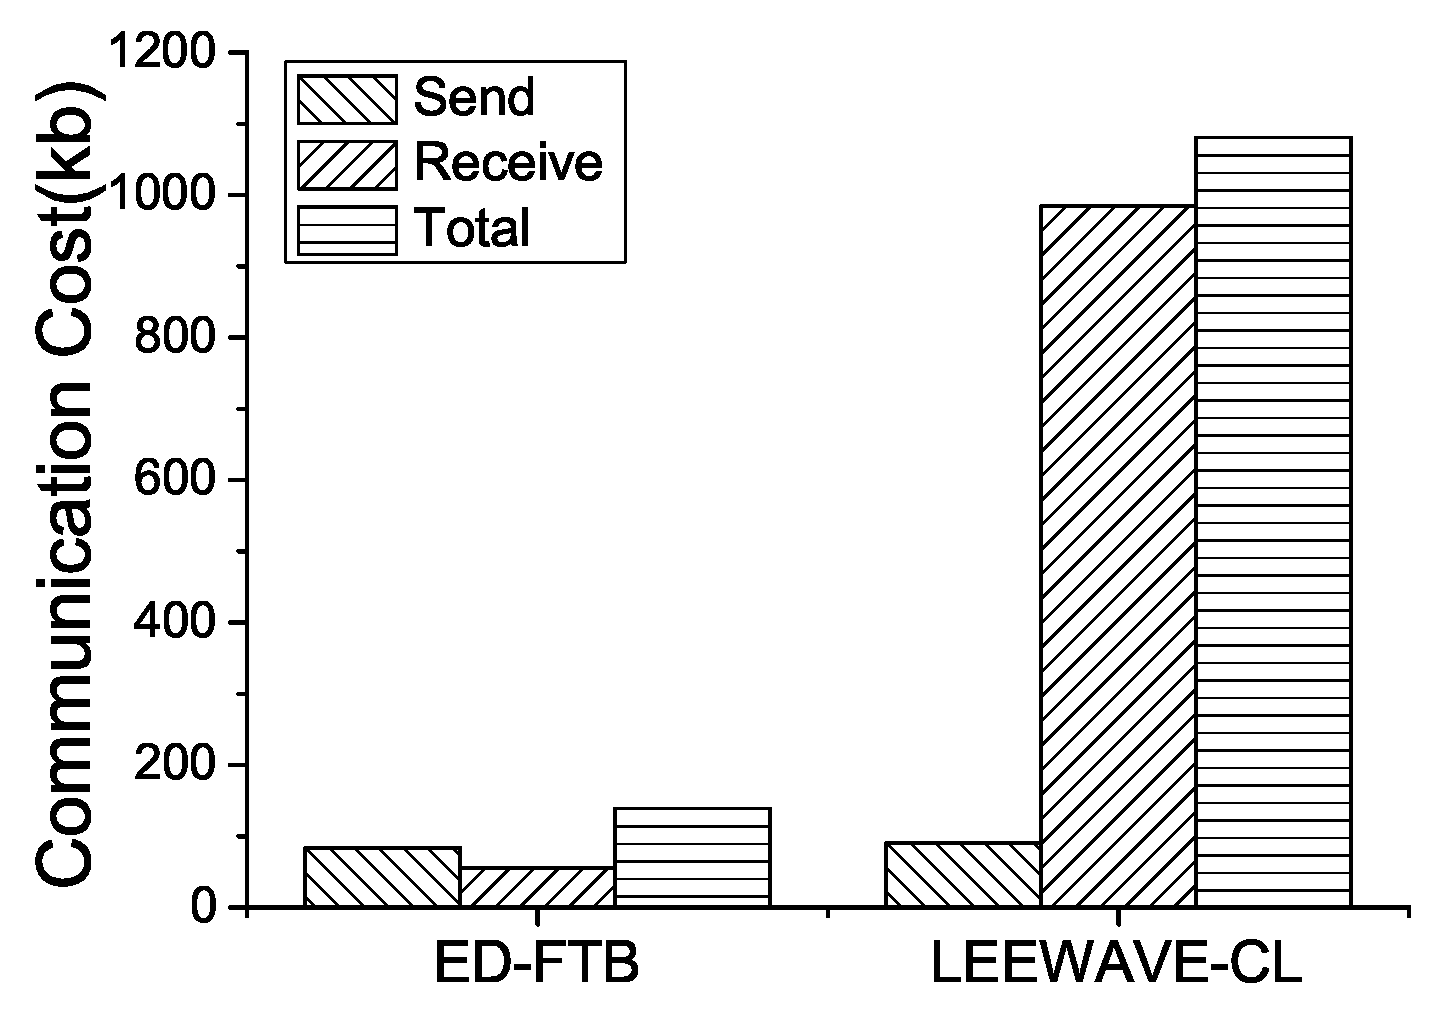
\includegraphics[width=2.7in]{Fig/chapter4/1k50m.eps}
	}
	\subfigure[$M=50,k=1,000$]{
		\label{50-1000}
		\includegraphics[width=2.7in]{Fig/chapter4/1000k50m.eps}
	}
	
	\subfigure[$M=200,k=1$]{
		\label{200-1}
		\includegraphics[width=2.7in]{Fig/chapter4/1k200m.eps}
	}
	\subfigure[$M=200,k=1,000$]{
		\label{200-1000}
		\includegraphics[width=2.7in]{Fig/chapter4/1000k200m.eps}
	}
	\vspace{-10pt}
	\caption{算法执行策略详细比较}
	\label{fig:components}
	\vspace{-0.5cm}
\end{figure}
接着,我们使用相同的界,对比了分析了本文所提查询策略与LEEWAVE所用查询策略对通信性能的影响。我们从协调者节点出发,研究了两种策略下它发送和接受的数据量以及总的数据通信开销。
图 \ref{fig:components}介绍了当$M$取50和$100$,k取$1$和$1000$下的实验结果。图中LEEWAVE-CL代表
结合了LEEWAVE的查询策略与本文的界特征后的算法。
从图中我们可以发现,协调者结点在两种策略下,发送的数据量差别不大且都比较小。这是因为,两个策略都有减少协调者数据发送的数据量这一共同目标。且两者使用的使用概要数据剪枝的策略很好的达成了这一目标。
但接受的数据量在两种策略下差别很大。ED-FTB所用的查询策略是在每个远程结点剪枝数据。每轮迭代完后远程结点仅需将所计算出来的局部最小的$k$个上界返回。而LEEAVE-CL需要将所有候选的跟计算界信息的两个算子返回。当远程结点所包含的数据越多,则两者的区别越大。特别地,当$k$值较小时(图 \ref{50-1} 和 \ref{200-1}),ED-FTB所收到的数据不到LEEWAVE-CL的十分之一。
%Especially, when $k$ is small(in Fig. \ref{50-1} and \ref{200-1}), the amount of data received in DT-KST is $10\%$ less than that of LEEWAVE-CL. 


\begin{figure}[t]
	\centering
		\centering
		\subfigure[$M=100$]{
			\label{fig:costM100}
			\includegraphics[width=2.7in]{Fig/chapter4/costM100.eps}
		}
		\subfigure[$M=1,000$]{
			\label{fig:costM1000}
			\includegraphics[width=2.7in]{Fig/chapter4/costM1000.eps}
		}
	\\
		\subfigure[$M=5,000$]{
		\label{fig:costM5000}
		\includegraphics[width=2.7in]{Fig/chapter4/costM5000.eps}
	}
		\subfigure[$M=10,000$]{
			\label{fig:costM10000}
			\includegraphics[width=2.7in]{Fig/chapter4/costM10000.eps}
		}
		\caption{$n$,$k$和$M$对ED-FTB算法通信开销的影响}
		\label{fig:costKM}
\end{figure}
其次,我们研究了$n$,$k$和$M$对ED-FTB算法通信开销的影响。在该组实验中,我们将$n$的值从256变化到$4,096$,将$k$的值从1变化到100。图\ref{fig:costKM}展示了不同$M$值下($M$从100编化到$10,000$),ED-FTB算法通信开销随参数变化的结果。首先,我们看出随着$k$值的增加,通信开销逐步增加。这是由于$k$值越大,每轮所剩候选数越多,候选所在的远程结点也就越多。从而每轮需要将概要数据发送到更多的候选结点中。其次,随着$n$值的增加通信开销也在增加。这是由于长轨迹需要发送更多的数据才能达到与短轨迹相同的剪枝效果。最后,对比三幅图可以发现,随着远程结点数据的增加,通信开销也在增加。这是由于在每轮迭代中,远程结点增加后,候选轨迹会分布到更多的结点中。因而,算法需要将概要数据发送到更多的结点中。因而总的通信开销也会增加。但是,对于极端情况$M=10,000$时,此时每个远程结点仅包含一条轨迹时我们的通信开销仍不到$10$Mb,远小于直接方法的开销(约$640$Mb)。因此,ED-FTB算法具有较高的通信节约性能。

\begin{figure}[t]
\centering
\subfigure[$k=1$]{
	\label{fig:costCmpk1}
	\includegraphics[width=2.7in]{Fig/chapter4/cmpk1.eps}
}
\subfigure[$k=10$]{
	\label{fig:costCmpk10}
	\includegraphics[width=2.7in]{Fig/chapter4/cmpk10.eps}
}
\\
\subfigure[$k=50$]{
	\label{fig:costCmpk50}
	\includegraphics[width=2.7in]{Fig/chapter4/cmpk50.eps}
}
\subfigure[$k=100$]{
	\label{fig:costCmpk100}
	\includegraphics[width=2.7in]{Fig/chapter4/cmpk100.eps}
}
\caption{算法性能比较}
\label{fig:costCmp}
\end{figure}
接下来,我们将ED-FTB与LEEWAVE和LEEWAVE-CL进行通信性能比较。在该组实验中我们将轨迹长度$n$从256变化到$4,096$。图\ref{fig:costCmp}展示了当$k$取值为1,10和100下的结果。从该组图中我们可以看出,本文所提ED-FTB算法性能最好,LEEWAVE-CL其次,最差的是LEEWAVE。LEEWAVE-CL比LEEWAVE好的原因是它使用了本文所提下界进行剪枝。本文所提下界由于比LEEWAVE中的更加紧凑,因而剪枝效果更好。最终导致通信开销更低。而ED-FTB算法比LEEWAVE-CL好的原因是,本文采用的是在远程结点剪枝的策略,只需发送概要数据。而LEEWAVE和LEEWAVE-CL 均是采用在协调者结点剪枝的策略,除了发概要数据还要发送和接受其他额外数据。因而开销更高。最后,我们可以发现,随着轨迹长度$n$和$k$值的增加,EDD-FTB算法所节省的通信开销逐步增大。这进一步说明了本文算法的优越性。

\subsection{算法可扩展性}
\begin{figure} [t]
	\centering
	\subfigure[Running time in respect of $n$,$N$]{
		\label{fig:KLN}
		\includegraphics[width=2.7in]{Fig/chapter4/edtimeScalability.eps}		
	}
	\subfigure[Communication cost in respect of  $n$,$N$]{
		\label{fig:MN}
		\includegraphics[width=2.7in]{Fig/chapter4/edcommScalability.eps}
	}
	\caption{ED-FTB 算法可扩展性 {(T-Big数据集)}}
	\label{fig:EDScalability}
\end{figure}

 本小节我们将在\emph{T-Big}数据集上从时间和通信两个角度研究了ED-FTB算法的可扩展性。首先,考虑了轨迹数量$N$(即数据量大小)和轨迹长度$n$对可扩展性的影响。
在该组实验中,我们将$k$设置为1,$M$设置为$10,000$。我们将轨迹长度从$256$到$4096$进行指数级变化,同时将轨迹数量从10万到1百万进行线性增加。
  图\ref{fig:EDScalability}分别对这两个角度的结果进行了介绍,其中图\ref{fig:KLN}介绍了时间性能受$n$和$N$的影响(时间包系统初始化过程中对数据进行哈尔小波转换的开销)。我们可以看到对于任意长度的轨迹数据集,ED-FTB算法的运行时间都随着轨迹数据量的增加而线性增加。
  此外,随着轨迹长度的指数增加,算法的运行时间也指数增加,即运行时间与轨迹长度呈一定的线性关系。这一结果反映了由于ED-FTB的剪枝效果较好,导致迭代结束后,所剩候选数较少。即我们对ED-FTB算法时间复杂度分析部分的$N'$较少。结合以上两点,我们可以看出ED-FTB算法运行时间随着数据集的大小而线性变换,因此运行效率具有较好的可扩展性。

\section{本章小结}\label{sec-c4-conclusion}
本章节介绍了利用FTB框架在嵌入欧式距离下的具体实现算法ED-FTB。本章节,首先针对欧式距离,提出了基于哈尔小波系数的概要数据。接着,提出了基于哈尔小波系数的欧式距离上、下界。
该上、下界能够随着小波粒度的增加而逐渐变紧,这使得我们利用将该距离嵌入到FTB框架称为可能。为此,我们提出了ED-FTB算法以实现基于欧式距离的查询。在我们的查询算法中,我们引入了边计算下界边剪枝的查询优化措施,以提高执行效率。通过在真实数据集上进行的实验,表明所提方法剪枝效果由于现有方案,且具有较好的可扩展性。

\section*{本章证明附件}\label{sec-c4-Appendix}
\textbf{引理 \ref{theory:dis}. }{\em 给定两条轨迹${\cal Q}$ 和 ${\cal C}$,$H{\cal Q}$ 和 $H{\cal C}$分别表示${\cal Q}$ 和 ${\cal C}$经过哈尔小波变换后的系数序列。我们有如下结论:$SED({\cal Q},{\cal C})=SED(H{\cal Q},H{\cal C})$。}
\begin{proof}
	首先,根据$S_{i}({\cal Q}, {\cal C})$ 和 $SED_{i}({\cal Q}, {\cal C})$定义(定义\ref{eq:basic})我们有
	\allowdisplaybreaks
	\begin{eqnarray}
	&&	S_{i+1}({\cal Q}, {\cal C})=\sum\nolimits_{j=0}^{2^{i+1}-1}SED(\va_{i+1,j}^{\cal Q},\va_{i+1,j}^{\cal C}) \nonumber \\
	&=&SED(\va_{i+1,0}^{\cal Q},\va_{i+1,0}^{\cal C}) + SED(\va_{i+1,1}^{\cal Q},\va_{i+1,1}^{\cal C}) + \cdots + \nonumber \\
	&\,& SED(\va_{i+1,2^{i+1}-2}^{\cal Q},\va_{i+1,2^{i+1}-2}^{\cal C}) + 	SED(\va_{i+1,2^{i+1}-1}^{\cal Q},\va_{i+1,2^{i+1}-1}^{\cal C}) \nonumber \\
	&=&SED(\va_{i,0}^{\cal Q},\va_{i,0}^{\cal C})  +   SED(\vd_{i,0}^{\cal Q}, \vd_{i,0}^{\cal C})   + \cdots+\nonumber \\
	&\,& SED(\va_{i,2^{i}-1}^{\cal Q},\va_{i,2^{i}-1}^{\cal C})  +   SED(\vd_{i,2^{i}-1}^{\cal Q}, \vd_{i,2^{i}-1}^{\cal C})  \nonumber   \nonumber \\
	&=& \sum\nolimits_{j=0}^{2^i-1}SED(\va_{i,j}^{\cal Q}, \va_{i,j}^{\cal C})+ \sum\nolimits_{j=0}^{2^i-1}SED(\vd_{i,j}^{\cal Q}, \vd_{i,j}^{\cal C})\nonumber \\
	&=&S_{i}({\cal Q}, {\cal C})+SED_{i}({\cal Q},{\cal C})
	\end{eqnarray}
	\allowdisplaybreaks[4]
根据如上公式,对于叶子层结点,我们有:
	\begin{eqnarray} \label{eq:prove1L}
	S_{L}({\cal Q},{\cal C})&=&S_{0}({\cal Q},{\cal C})+ \sum\nolimits_{i=0}^{L-1}{SED_{i}({\cal Q},{\cal C})} \nonumber \\
	&=& SED(H{\cal Q},H{\cal C})
	\end{eqnarray}
	此外,第$L$层为叶子节点层,包含了轨迹的原始信息。所以我们又有$SED({\cal Q},{\cal C}) = S_{L}({\cal Q},{\cal C})$。此时结合公式\ref{eq:prove1L}
	我们得到 $SED({\cal Q},{\cal C})=SED(H{\cal Q},H{\cal C})$。原问题得证。
\end{proof}

\textbf{定理 \ref{theory:lower}. }{\em $HLB$会随着粒度的概要数据粒度的增加而逐渐上升,即$HLB_{l} \le HLB_{l+1}$。}
至此,我们根据哈尔小波变换得到原始轨迹不同粒度概要数据,并根据概要数据提出了欧式距离的上、下界。


\begin{proof}\label{proof:p2}
	我们的策略是证明 $HLB_{l+1}- HLB_{l}\ge 0$。我们首先将其左半部分展开:
	\begin{eqnarray}\label{eq:minus}
HLB_{l+1}- HLB_{l}= SED_{l+1}({\cal Q},{\cal C}) - \sum\nolimits_{j=0}^{2^{l+1}-1}(||\vd_{l+1,j}^{\cal Q}||^2  + ||\vd_{l+1,j}^{\cal C}||^2)+\nonumber\\
 2(\sqrt{\sum_{i=l+1}^{L -1}\sum_{j=0}^{2^i-1}||\vd_{i,j}^{\cal Q}||^2} \cdot \sqrt{\sum_{i=l+1}^{L -1}\sum_{j=0}^{2^i-1}||\vd_{i,j}^{\cal C}||^2} -\sqrt{\sum_{i=l+2}^{L -1}\sum_{j=0}^{2^i-1}||\vd_{i,j}^{\cal Q}||^2} \cdot \sqrt{\sum_{i=l+2}^{L -1}\sum_{j=0}^{2^i-1}||\vd_{i,j}^{\cal C}||^2})\nonumber
	\end{eqnarray}	
	接着, 我们将$SED_{l+1}({\cal Q},{\cal C})$ 展开得到$SED_{l+1}({\cal Q},{\cal C})=\sum_{j=0}^{2^{l+1}-1}{(||\vd_{l+1,j}^{\cal Q}||^2+||\vd_{l+1,j}^{\cal C}||^2}-2 \vd_{l+1,j}^{\cal Q} \bigcdot \vd_{l+1,j}^{\cal C})$。我们的问题变为证明如下不等式成立。
	\begin{eqnarray}\label{eq:InEq}
	\sum_{j=0}^{2^{l+1}-1}\vd_{l+1,j}^{\cal Q} \bigcdot \vd_{l+1,j}^{\cal C} &\le& \sqrt{\sum_{i=l+1}^{L-1}\sum_{j=0}^{2^i-1}||\vd_{i,j}^{\cal Q}||^2} \cdot \sqrt{\sum_{i=l+1}^{L-1}\sum_{j=0}^{2^i-1}||\vd_{i,j}^{\cal C}||^2} \nonumber\\
&\quad&	-	\sqrt{\sum_{i=l+2}^{L-1}\sum_{j=0}^{2^i-1}||\vd_{i,j}^{\cal Q}||^2} \cdot \sqrt{\sum_{i=l+2}^{L-1}\sum_{j=0}^{2^i-1}||\vd_{i,j}^{\cal C}||^2} 
	\end{eqnarray}	
	对于不等式 \ref{eq:InEq}的左半部分我们有
	$\sum_{j=0}^{2^{l+1}-1}\vd_{l+1,j}^{\cal Q}\bigcdot \vd_{l+1,j}^{\cal C} \le
	\sqrt{\sum_{j=0}^{2^{l+1}-1}||\vd_{l+1,j}^{\cal Q}||^2} \cdot \sqrt{\sum_{j=0}^{2^{l+1}-1}||\vd_{l+1,j}^{\cal C}||^2}$。
	所以我们的目标变为证明
	$\sqrt{\sum_{j=0}^{2^{l+1}-1}||\vd_{l+1,j}^{\cal Q}||^2} \cdot \sqrt{\sum_{j=0}^{2^{l+1}-1}||\vd_{l+1,j}^{\cal C}||^2}$
	小于不等式\ref{eq:InEq}的右半部分。
	为方便表示,我们令$x= \sum_{j=0}^{2^{l+1}-1}||\vd_{l+1,j}^{\cal Q}||^2$,$y=\sum_{j=0}^{2^{l+1}-1}||\vd_{l+1,j}^{\cal C}||^2$,$\alpha = \sum_{i=l+2}^{L-1}\sum_{j=0}^{2^l-1}||\vd_{i,j}^{\cal Q}||^2$,$\beta =  \sum_{i=l+2}^{L-1}\sum_{j=0}^{2^l-1}||\vd_{i,j}^{\cal C}||^2$。
	则不等于\ref{eq:InEq}等价于:
	\begin{eqnarray}\label{eq:sim}
	\sqrt{x \cdot y} + \sqrt{\alpha \cdot \beta} \le \sqrt{(\alpha+x) \cdot (\beta+y)}
	\end{eqnarray}	
	我们将如上不等式两边平方得到如下不等式:
	\begin{eqnarray}\label{eq:final}
	2\sqrt{x\cdot y \cdot \alpha \cdot \beta} \le \alpha \cdot y+\beta\cdot x
	\end{eqnarray}	
	根据算数-几何平均不等式,我们得不等式\ref{eq:final} 成立。原问题得证。
\end{proof}

%% Property 2
\textbf{定理 \ref{theory:upper}. }{\em $HUB$会随着粒度的概要数据粒度的增加而逐渐下降,即$HUB_{l+1} \le HLB_{l}$。}
\begin{proof}
	我们的策略是证明 $HUB_{l+1}- HUB_{l}\le 0$。我们首先将其左半部分展开:
	\begin{eqnarray}\label{eq:minusupper}
	HUB_{l+1}- HUB_{l}= SED_{l+1}({\cal Q},{\cal C}) - \sum\nolimits_{j=0}^{2^{l+1}-1}(||\vd_{l+1,j}^{\cal Q}||^2  + ||\vd_{l+1,j}^{\cal C}||^2) -\nonumber\\
	2(\sqrt{\sum_{i=l+1}^{L -1}\sum_{j=0}^{2^i-1}||\vd_{i,j}^{\cal Q}||^2} \cdot \sqrt{\sum_{i=l+1}^{L -1}\sum_{j=0}^{2^i-1}||\vd_{i,j}^{\cal C}||^2} -\sqrt{\sum_{i=l+2}^{L -1}\sum_{j=0}^{2^i-1}||\vd_{i,j}^{\cal Q}||^2} \cdot \sqrt{\sum_{i=l+2}^{L -1}\sum_{j=0}^{2^i-1}||\vd_{i,j}^{\cal C}||^2})\nonumber
	\end{eqnarray}	
		接着, 我们将$SED_{l+1}({\cal Q},{\cal C})$ 展开得到$SED_{l+1}({\cal Q},{\cal C})=\sum_{j=0}^{2^{l+1}-1}{(||\vd_{l+1,j}^{\cal Q}||^2+||\vd_{l+1,j}^{\cal C}||^2}-2 \vd_{l+1,j}^{\cal Q} \bigcdot \vd_{l+1,j}^{\cal C})$。我们的问题变为证明如下不等式成立。
	\begin{eqnarray}\label{eq:InEqUB}
	\sum_{j=0}^{2^{l+1}-1}\vd_{l+1,j}^{\cal Q} \bigcdot \vd_{l+1,j}^{\cal C} &\ge&
	\sqrt{\sum_{i=l+2}^{L-1}\sum_{j=0}^{2^i-1}||\vd_{i,j}^{\cal Q}||^2} \cdot \sqrt{\sum_{i=l+2}^{L-1}\sum_{j=0}^{2^i-1}||\vd_{i,j}^{\cal C}||^2} \nonumber\\
	&\quad&	-		 \sqrt{\sum_{i=l+1}^{L-1}\sum_{j=0}^{2^i-1}||\vd_{i,j}^{\cal Q}||^2} \cdot \sqrt{\sum_{i=l+1}^{L-1}\sum_{j=0}^{2^i-1}||\vd_{i,j}^{\cal C}||^2} 
	\end{eqnarray}	
	由于	$\sum_{j=0}^{2^{l+1}-1}\vd_{l+1,j}^{\cal Q}\bigcdot \vd_{l+1,j}^{\cal C} \ge
-	\sqrt{\sum_{j=0}^{2^{l+1}-1}||\vd_{l+1,j}^{\cal Q}||^2} \cdot \sqrt{\sum_{j=0}^{2^{l+1}-1}||\vd_{l+1,j}^{\cal C}||^2}$,所以我们的问题变为证明$-\sqrt{\sum_{j=0}^{2^{l+1}-1}||\vd_{l+1,j}^{\cal Q}||^2} \cdot \sqrt{\sum_{j=0}^{2^{l+1}-1}||\vd_{l+1,j}^{\cal C}||^2} $大于公式\ref{eq:InEqUB}右半部分。与定理\ref{theory:lower}证明类似,我们令$x= \sum_{j=0}^{2^{l+1}-1}||\vd_{l+1,j}^{\cal Q}||^2$,$y=\sum_{j=0}^{2^{l+1}-1}||\vd_{l+1,j}^{\cal C}||^2$,$\alpha = \sum_{i=l+2}^{L-1}\sum_{j=0}^{2^l-1}||\vd_{i,j}^{\cal Q}||^2$,$\beta =  \sum_{i=l+2}^{L-1}\sum_{j=0}^{2^l-1}||\vd_{i,j}^{\cal C}||^2$。
	则不等于\ref{eq:InEqUB}等价于:
	\begin{eqnarray}\label{eq:simUB}
	- \sqrt{x \cdot y} \ge  \sqrt{\alpha \cdot \beta}  -  \sqrt{(\alpha+x) \cdot (\beta+y)} 
% \sqrt{(\alpha+x) \cdot (\beta+y)} \le 	\sqrt{x \cdot y} + \sqrt{\alpha \cdot \beta} 
	\end{eqnarray}	
	不等式经过变换可得到不等式\ref{eq:sim}。因此可得不等式\ref{eq:InEqUB}成立,原问题得证。
\end{proof}


\clearpage
\phantom{s}
\clearpage
\chapter{FLB框架的应用}\label{chapter:FLBDTW}

本章主要介绍如何使用FLB框架处理基于动态时间卷曲距离的查询。首先,章节\ref{sec-c5-DTWsummary}介绍了利用包围信封为DTW距离提供概要数据。 然后,章节\ref{sec-c5-lowerBound}介绍了基于包围信封的DTW距离下界。其次,章节\ref{sec-c5-algorithm}介绍了算法DTW-FLB,以处理当使用动态时间卷曲距离作为距离度量准则时的查询。接着,章节\ref{sec-c5-algorithm}展示了DTW-FLB算法的有效性和可扩展性。再其次,章节 \ref{sec-c5-conclusion}小结本章的研究内容。最后,本章涉及到的证明内容放在附件部分。


\section{基于动态时间卷曲距离的概要数据}\label{sec-c5-DTWsummary}

\subsection{基于动态时间卷曲距离的轨迹相似度度量}\label{sec-c5-DTW}
\begin{figure}[t]
	\centering
	\includegraphics[width=0.48\textwidth]{Fig/chapter5/DTW}
	\caption{带约束的动态时间卷曲}
	\label{fig:DTW}
\end{figure}
给定查询轨迹$\cal Q$表示为${\cal Q}=\{\vq_{0}, \vq_{1}, \cdots, \vq_{n-1}\}$,以及一条候选轨迹$\cal C$表示为${\cal C}=\{\vc_{0}, \vc_{1}, \cdots, \vc_{n-1}\}$,其中$n$为轨迹长度,每个轨迹点来自$d$维空间,即$\vq_{i},\vc_{i} \in R^{d}$。为使用动态时间卷曲距离匹配 $\cal Q$和$\cal C$,我们构建了一个$n\times n$的代价矩阵$cost$。其中第$i$行第$j$列的元素记录了使用欧式距离匹配$\vq_{i}$和$\vc_{j}$两点之间的代价。动态时间卷曲距离的目的就是发现一条从如图\ref{fig:DTW}所示左下角出发到右上角结束的代价最小的路线/卷曲路径。一条卷曲路径需满足如下3个特别的约束:
\begin{itemize}
	\item \textbf{边界条件}: 路径从代价矩阵的$[0,0]$号格子出发并在$[n-1,n-1]$号格子结束。
	
	\item \textbf{连续性}: 如果路径中相邻的两次权重值分别取自代价矩阵的$[i,j]$ 和 $[i^{'},j^{'}]$两个单元,那么这两个单元的位置关系必满足如下条件:$i^{'}-i\le 1$ 和 $j^{'} - j \le 1$。这个约束使得路径在扩展过程中只能从一个格子扩展到其半径为1周边的格子。
	\item \textbf{单调性}: 如果路径中相邻的两次权重值分别取自代价矩阵的$[i,j]$ 和 $[i^{'},j^{'}]$两个单元,那么这两个单元的位置关系还须满足如下条件: $i^{'}-i\ge 0$ 和 $j^{'} - j \ge 0$。这个约束使得路径搜索过程中只能前进不能后退。
\end{itemize}
根据以上描述,我们形式化给出动态时间卷曲距离的定义:
\begin{eqnarray}\label{eq:dtwDef}
DTW({\cal Q}, {\cal C})= \min{\sum\nolimits_{k=1}^{K}\vw_{k}} \qquad {(n\le K < 2n)}
\end{eqnarray}
其中,$\vw_{k}$是卷曲路径$\cal W$的第$k$个元素,其值来源于代价矩阵的第$[i,j]$个格子。
$\cal{W}=\{$ $\vw_{1}$$,\vw_{2}$$,\cdots,\vw_{K}\}$, 代表了一条匹配$\cal{Q}$ 和 $\cal{C}$卷曲路径。

动态时间卷曲距离的计算过程可通过动态规划算法实现,因为其计算过程可以看作如下最优子结构的递归:
\begin{eqnarray}\label{eq:dtwdef}
DTW&=&\gamma(n-1,n-1) \\ \nonumber
\gamma(i,j)&=&SED(\vq_{i}, \vc_{j}) + \min(\gamma(i-1,j-1), \gamma(i-1,j), \nonumber \\
&&\gamma(i,j-1))  \quad s.t.  \quad |i-j| \le \delta
\end{eqnarray}
其中$\delta$ 是一个全局约束,用于限制查询路径的可以偏离对角线的范围。图\ref{fig:DTW}中显示了当$\delta=4$时,灰色部分即为卷曲路径的查询范围。
使用全局约束的原因有两个:(i)该约束可以提高查询的效率,$\delta$使得动态时间卷曲距离的计算复杂度由原来的$n^2$降低为$\frac{n^2}{\delta}$。
(ii)该约束还能有效抑制无效的卷曲路径的产生。比如,一轨迹的一小段匹配到另一轨迹的一大段上情况。


\subsection{基于包围信封的概要数据}\label{sec-c5-BE}
\begin{figure}[t]
	\centering
	\includegraphics[width=0.48\textwidth]{Fig/chapter5/BE}
	\caption{包围信封}
	\label{fig:BE}
\end{figure}
包围信封(Bounding Envelope,BE)概念来源于时间序列数据分析,其目的是使用一上一下两条边界曲线来包住给定的时间序列。如图\ref{fig:BE}所示,红色虚线为一条时间序列,$U$和$L$两条线分别代表了这条时间序列的上界和下界。给定时间序列,构造其包围信封的方法有许多。由于本文的目的是利用包围信封构造概要数据,故所构造的包围信封包含的数据量要低。此外,所构造的包围信封还应具有多粒度特性,以适应FLB框架的需求。

为此,引入基于时间序列划分(Time Series Segmentation)的包围信封。其做法是给定一条时间序列$\cal S$,将其均匀划分成多个等长度的片段。我们使用$s_{l}^{p}= {[lb, ub, len]}$来表示其中一条片段$\{\vq_{i}, \vq_{i+1}, \cdots, \vq_{j} \}$的最小包围盒(Minimum Bounding Rectangle, MBR)。其中$l$代表划分的粒度(粒度越细,每个片段的长度越短),$p$代表该片段在当前划分下所对应的位置。$lb$ 和 $ub$分别代表该片段的最小值和最大值,$len$代表该片段的长度。由$\{s_{l}^{1}, \cdots s_{l}^{n'}\}$所构成的列表代表了该次划分所对应的包围信封,其用${\cal S}_{l}$表示。在第0层,整个时间序列被看做一个划分,接着将其均匀切成$R$个不相交的相连子片段。这个过程可以一直持续下去,直到每个片段的长度为1截止。

\begin{table}[t]
	\centering  
	\renewcommand\arraystretch{1.2}
	\begin{tabular}{|c|c|c|c|c|c|c|c|c|} 
		\hline
		${\cal S}_{0}$ &  \multicolumn{4}{|c|}{$s_{0}^{0}={[2,5,4]}$} \\ \hline
		${\cal S}_{1}$ & \multicolumn{2}{|c|}{$s_{1}^{0}={[2,5,2]}$} & \multicolumn{2}{|c|}{$s_{1}^{1}={[3,4,2]}$} \\ \hline 
		${\cal S}_{2}$ & \multicolumn{1}{|c|}{$s_{2}^{0}={[5,5,1]}$} & \multicolumn{1}{|c|}{$s_{2}^{1}={[2,2,1]}$} &
		\multicolumn{1}{|c|}{$s_{2}^{2}={[4,4,1]}$} &  \multicolumn{1}{|c|}{$s_{2}^{3}={[3,3,1]}$} \\ \hline 
		$Q$ & 5 & 2 & 4 & 3
		\\ \hline
	\end{tabular}
	\caption{时间序列$\cal S$的多粒度包围盒}
	\label{table:BE}
\end{table}
表格\ref{table:BE}介绍了给定时间序列${\cal S}=\{5,2,4,3\}$,计算其不同粒度包围盒的过程。其中,$R$的值设置为2。即从粗粒度到细粒度切分的过程中,每次将一个片段均匀划分成2个子片段。不失一般性,接下来的示例和实验室中,我们都将$R$的值设置为2。值得注意的是,本文采用的划分为均匀划分,而相关文章中所提非均匀划分的方法也可以被使用。此外,由于是均匀划分,我们可以推算出每个片段的长度,故其值无需保存。
 

%
%为适应动态时间卷曲计算和FLB所要求的概要数据具有多粒特性这两个需求,本文首先使用如下方法为给定的查询轨迹 $\cal Q$构造包围信封。
%\begin{eqnarray}\label{eq:dtwUL}
%{\cal U} = \{\vu_{0},\vu_{1},\cdots, \vu_{n-1} \} &,& \forall j  \, \vu_{i}^{j}=\max(\vq_{i-\delta}^{j} : \vq_{i+\delta}^{j}) \nonumber \\
%{\cal L} = \{\vl_{0},\vl_{1},\cdots, \vl_{n-1} \}&,& \forall j  \, \vl_{i}^{j}=\min(\vq_{i-\delta}^{j} : \vq_{i+\delta}^{j})
%\end{eqnarray}
%其中${\cal U}$ 和 ${\cal L}$分别对应了轨迹的上边界和下边界,$\delta$是动态时间卷曲距离计算中的全局约束。接下来,我们设计了基于$\cal U$和$\cal L$的多粒度包围信封。
%
%Here, ${\cal U}$ and ${\cal L}$ are the sequences of  upper and lower boundaries, and $\delta$ is the warping constraint of DTW.  Next, we design different degrees of approximation for the bounding envelope in Eq.  \ref{eq:hatUL}. 


\section{动态时间卷曲距离的下界}\label{sec-c5-lowerBound}
 本节将介绍如何根据包围信封计算动态时间卷曲距离的下界。首先将介绍点的上、下界,然后再介绍如何利用点的范围计算轨迹的下界。
 
\subsection{满足DTW约束的包围信封及下界} 
令 $\vq$ 和 $\vc$ 表示两个来自$d$维实数空间的点, 其中$\vc$的值已知,$\vq$的值不知道,但知道其在一个$d$维矩形$\{\vu, \vl\}$里,即$\forall j\in [0, d),  \,\, {\vl}^{j}  \le \vq^{j} \le \vu^{j}$。对$\vq$ 和 $\vc$之间的实际欧式距离我们无法计算出来,但可以通过如下引理计算出距离的下界。
\begin{lemma}\label{theory:SEDLB}
	给定 $\bq$ 、$\bc$ 以及$\bq$的包围矩形$\{\bu, \bl\}$,我们有
	$SED\_LB(\{{\bu},\bl \},\bc)\le SED(\bq,\bc)$, 其中 $SED\_LB(\{{\bu},\bl \},\bc)$ 的计算过程如下:
	\allowdisplaybreaks
	\begin{equation}
	SED\_LB(\{{\bu},\bl \},\bc) =
	\sum_{j=0}^{d-1} \begin{cases}
	({\bc}^{j}- {\bu}^{j})^2 & \emph{if} \,\,\,   \bu^{j} \le {\bc}^{j},\\
	\quad 0 &   \emph{if} \,\,\,  \bl^{j} \le  {\bc}^{j} \le \bu^{j},\\
	({\bl}^{j} -{\bc}^{j})^2 & \emph{if} \,\,\,    {\bc}^{j} \le \bl^{j}.\\
	\end{cases}
	\end{equation}
	\allowdisplaybreaks[4]
\end{lemma}

接着介绍如何构建满足动态时间卷曲距离的包围信封。根据包围信封的介绍,我们知道给定查询轨迹$\cal Q$,构建包围信封的最重要就是构造轨迹的上、下边界。同时,考虑到动态时间卷曲距离的全局约束特性。我们使用如下方法构建轨迹的上、下边界:
We next introduce how to construct a bounding envelope $\{{\cal U},{\cal L}\}$ for trajectory $\cal Q$, as defined below. %In Eq. \ref{eq:dtwUL},  ${\cal U}$ and 
\begin{eqnarray}\label{eq:dtwUL}
{\cal U} = \{\vu_{0},\vu_{1},\cdots, \vu_{n-1} \} &,& \forall j  \, \vu_{i}^{j}=\max(\vq_{i-\delta}^{j} : \vq_{i+\delta}^{j}) \nonumber \\
{\cal L} = \{\vl_{0},\vl_{1},\cdots, \vl_{n-1} \}&,& \forall j  \, \vl_{i}^{j}=\min(\vq_{i-\delta}^{j} : \vq_{i+\delta}^{j})
\end{eqnarray}
公式\ref{eq:dtwUL}中,${\cal U}$ 和 ${\cal L}$分别代表轨迹的上边界和下边界, $\delta$ 为动态时间卷曲距离中的全局约束。根据如上方式计算出来的包围盒,我们称之为满足动态时间卷曲约束的包围信封(Dynamic Time Warping constraint Bounding Envelope,DTWBE)。
此时,根据DTWBE$\{{\cal U}, {\cal L}\}  $和$\cal C$,我们可以给出如下距离定义:
\begin{equation}\label{eq:LBKeogh}
LB\_Keogh({\{\cal U,\cal L\},{\cal C}})=  \sum\nolimits_{i=0}^{n-1}	SED\_LB(\{{\vu_{i}},\vl_{i} \},\vc_{i})
\end{equation}
该定义可以看做是原始一维的$LB\_Keogh$下界在多维情况下的扩展,并得到如下下界定理:
\begin{theorem}\label{theorem:DTWLBK}
	给定轨迹$C$和待查询轨迹$Q$满足动态时间卷曲约束的包围信封$\{{\cal U}, {\cal L}\}$,我们有如下结论: $LB\_Keogh({\{\cal U,\cal L\},{\cal C}}) \le DTW(Q,C)$。
\end{theorem}


\subsection{基于多粒度包围信封的下界} 
为计算上一小节介绍的$LB\_Keogh$下界,需要传递DTWBE,其数据量为$2*n$。因此,不满足我们降低通信的目标。为此,本文首先设计了基于DTWBE的多粒度包围信封。多粒度信封的第$l$层边界计算方式如下:
%Let $\{\hat{{\cal U}}_l, \hat{{\cal L}}_l\}$ denote the level-$l$ approximation of boundaries ${\cal U}$ and ${\cal L}$ respectively. 
\begin{eqnarray}\label{eq:hatUL}
\hat{{\cal U}}_l =\{ \hat{\vu}_{l,0}, \hat{\vu}_{l,1},\cdots, \hat{\vu}_{l,2^l-1}\}  &,&
\forall j  \, \hat{\vu}_{l,i}^{j}=\max(\vu_{i\cdot 2^{L-l}}^{j} : \vu_{(i+1)\cdot 2^{L-l}-1}^{j})  \nonumber \\
\hat{{\cal L}}_l=\{\hat{\vl}_{l,0}, \hat{\vl}_{l,1},\cdots, \hat{\vl}_{l,2^l-1}\}   &,&
\forall j  \, \hat{\vl}_{l,i}^{j}=\min(\vl_{i\cdot 2^{L-l}}^{j} : \vl_{(i+1)\cdot 2^{L-l}-1}^{j})
\end{eqnarray}	
第$l$层的包围信封计算过程可看作将原来的DTWBE均匀切分成$2^l$块,然后对每个信封块计算仅使用两个$d$维点来构成新的包围信封。根据对公式 \ref{eq:hatUL}的观察,我们得到两种结论:(i)第$l$层的包围信封$\{\hat{{\cal U}}_{l}, \hat{{\cal L}}_{l}\}$ 数据量是第$l-1$层的两倍;(ii)第$l-1$层的数据被第$l$层包含。因此,在由粗到细发送包围信封这一概要数据时,除第$0$层外,其他层只需要发送一半的信息量(这一半数据的每个值需要用0和1标注其位置是在左边还是右边,但位置信息消耗的开销较小可忽略)。
那么假定远程结点已获取到查询轨迹$\cal Q$的第$l$层包围信封$\{\hat{{\cal U}}_l,\hat{{\cal L}}_l\}$,我们可通过如下公式来计算给定的候选与$\cal Q$的下界。
\begin{theorem}\label{theo:HPAA}
	给定轨迹$\cal Q$的第$l$层包围信封$\{\hat{{\cal U}}_{l}, \hat{{\cal L}}_{l}\}$和候选轨迹$\cal C$,我们得到如下结论:
	 $LB\_HPAA({  \{\hat{{\cal U}_{l}}, \hat{{\cal L}_{l}}\},\overline{{\cal C}}_{l}}) \le DTW(\cal Q, \cal C)$。其中$LB\_HPAA$的计算公式如下:
	 \begin{eqnarray}\label{bound:HPAA}
	 LB\_HPAA({\{\hat{{\cal U}_{l}}, \hat{{\cal L}_{l}}\},\overline{{\cal C}}_{l}})= 2^{L-l} \cdot \sum_{i=0}^{2^{l}-1} SED\_LB(\{ \hat{\bu}_{l,i}, \hat{\bl}_{l,i} \}, \bar{\bc}_{l,i})\nonumber
	 \end{eqnarray}
\end{theorem}
以上定理说明了给定查询轨迹的第$l$层包围信封和候选误轨迹差树的第$l$层均值,就能为原始轨迹和候选轨迹计算出动态时间卷曲距离的下界。同时该下界的计算复杂度是线性的,远小于距离本身二次的复杂度。因此,通过计算下界可为剪枝候选提供帮助。

此外,为配合FLB框架,我们需要证明,$LB\_HPAA$能随着粒度的增加而逐渐变紧。为此我们给出如下定理:
\begin{theorem}\label{theo:DTWLbInc}
	$LB\_HPAA$下界能随着查询轨迹包围信封层次的增加而逐渐变紧。
	也就是说: $LB\_HPAA({  \{\hat{{\cal U}_{l}}, \hat{{\cal L}_{l}}\},\overline{{\cal C}}_{l}})\le  LB\_HPAA({  \{\hat{{\cal U}}_{l+1}, \hat{\cal L}_{l+1}\},\overline{\cal C}_{l+1}})$。
\end{theorem}

%\textbf{是否可以构造上界?}
%至此为止,我们已经构造出了动态时间卷曲距离的下界。我们通过上一章知道如果能同时获取上界 尝试通过相同的概要数据计算出上界。


\section{基于动态时间距离的查询算法:DTW-FLB}\label{sec-c5-algorithm}
\subsection{DTW-FLB算法实现}
在上一节,我们已经利用多粒度概要数据得到越来越紧的动态时间卷曲距离下界。这使得在FLB框架中插入欧式距离成为可能。本节将详细介绍动态时间卷曲距离跟FLB相结合的查询算法DTW-FLB。DTW-FLB维持了FLB框架的主要结构,只对本章第一节所介绍的接口进行了具体实现。

\begin{algorithm}[t]
	\renewcommand{\baselinestretch}{1}
	\caption{{\sl DTW-FLB在协调者节点} \label{alg:DTWCor}}
	\begin{algorithmic}[2]
		\STATE /* \emph{DTW-FLB协调者结点函数接口实现} */
	\end{algorithmic}
	\textbf{coordinatorInit}(${\cal Q}, {\cal R}$)
	\begin{algorithmic}[1]
		\STATE 根据公式\ref{eq:dtwUL}构建DTWBE $\{{\cal U},{\cal L}\}$;
		 \FOR{$i=1$,$i<\log_{2}n$;$i++$}
			 \STATE 根据公式\ref{eq:hatUL}构建第$i$层包围信封 $ \{\hat{{\cal U}_{l}}, \hat{{\cal L}_{l}}\}$;
		\ENDFOR 
		\STATE $l\leftarrow -1$;
	\end{algorithmic}
	\textbf{generateInfo()}
	\begin{algorithmic}[1]
		\STATE $l\leftarrow l+1$; 
		\STATE \textbf{return} $ \{\hat{{\cal U}_{l}}, \hat{{\cal L}_{l}}\}$;
	\end{algorithmic}
\end{algorithm}

\begin{algorithm}[t]
	\renewcommand{\baselinestretch}{1}
	\caption{{\sl DTW-FLB在远程结点} \label{alg:DTWRemote}}
	\begin{algorithmic}[2]
		\STATE /* \emph{DTW-FLB远程结点函数接口实现} */
	\end{algorithmic}
	\textbf{remoteInit($TS_{r} , S_{r}$)}
	\begin{algorithmic}[1]
		\IF{第一次接受查询}
			\STATE 构建R-Tree索引。
			\FORALL{ $\cal C$ in $TS_{r}$}
				\STATE $\overline{\cal C} \leftarrow$  $\cal C$的均值序列; \COMMENT{候选轨迹获取所有层的均值构成的序列}
			\ENDFOR 
		\ENDIF
		\FORALL{ $\cal C$ in $TS_{r}$}
		\STATE $C\_BF \leftarrow 0$;  \COMMENT {为$\cal C$初始化下界}
		\STATE $S_{r}=S_{r} \cup C\_BF$;
		\ENDFOR
	\end{algorithmic}
	%(line \ref{a3:info} in Alg. \ref{alg:F2Co})
	\textbf{updateBounds}($S_{r}$, $m$) \qquad  $/*m=\{ \hat{\vu}_{l,i}, \hat{\vl}_{l,i} \}*/$
	\begin{algorithmic}[1]
		\IF{$l==0$}
			\STATE 使用索引树进行剪枝。
		\ENDIF
		\FORALL{ $\cal C$ in $TS_{r}$}
			\STATE $factor =2^{L-l}$;
			\STATE $c.lb=0$;
			 \FOR{$i=0$,$i<2^{l}$;$i++$}
					\STATE $p\_lb=SED\_LB(\{ \hat{\vu}_{l,i}, \hat{\vl}_{l,i} \}, \bar{\vc}_{l,i})$;
					\STATE $c.lb+=p\_lb$;
					\IF{$c.lb>\theta$}
						\STATE 将该轨迹从$S_{r}$中移除;
					\ENDIF
			\ENDFOR 
			\STATE 将$\cal C$的下界更新为$c.lb$;
		\ENDFOR
	\end{algorithmic}
\end{algorithm}
我们首先介绍如何实现那些运行在协调者节点的上的函数。在\textsf{coordinatorInit}函数中,我们首先对待查询轨迹计算出对应的DTWBE,接着基于DTWBE,我们构造多粒度的包围信封(即概要数据)。
由于FLB框架也是迭代式由粗到细的通信计算框架,在每轮的迭代中会将某一层的概要数据(包围信封)发送给远程结点。因此,在初始化过程中我们用$l$来记录当前已经发送到哪一层的数据,并将$l$初始化为$-1$,以便从第0层开始发送。此外,我们在\textsf{generateInfo}中准备将要发送的下一层概要数据,以便协调者结点发送。在发送数据时需要注意的是,由于$ \{\hat{{\cal U}_{l}}, \hat{{\cal L}_{l}}\}$的一半数据量已经包含在 $\{\hat{{\cal U}}_{l-1}, \hat{{\cal L}}_{l-1}\}$中,我们只需传输剩下的一半数据。


接着,介绍运行在远程结点的函数。对于\textsf{RemoteInit}函数,若远程结点是第一次接受查询,则会为每条候选轨迹进行哈尔小波变换。若不是,则为该结点所包含的每条轨迹初始化界特征信息(下界初始化为0,不记录上界)。在查询执行过程中\textsf{UpdateBounds}函数为候选更新下界。直接实现方式为根据下界的计算公式直接算出该值。但由于查询过程中的主要计算开销就是对所有候选更新界特征。因此,降低该过程的计算开销很有必要。
为降低更新界特征的计算开销,与上一章一样采用在更新界过程中进行剪枝的思想。根据$LB\_HPAA$的定义,我们可知该下界是一系列点距离下界的累加和。由于每个点距离下界都是大于0的数,因此我们可以在累加的过程中,通过判断当前已经累加的值是否已经超过剪枝的阈值。若超过了 则可提前将该值过滤掉。

除了以上步骤外,我们引入了R-tree来对轨迹构建索引以提高查询效率。具体地:首先,每个远程结点对自己局部轨迹数据构建R-tree索引。接着,当该结点第$0$层包围信封时,使用R-tree来剪枝。剪枝具体过程入下:(i) 遍历R-tree,找到跟查询轨迹包围信封相交的叶子节点。(ii)遍历这些叶子节点所包含的轨迹,并将这些轨迹列为候选。


 \subsection{DTW-FLB算法性能分析}
 本章节将从时间复杂度和空间复杂度量方面 对DTW-FLB进行性能分析。在此之前,我们仍使用$|C_{i}|$ 和 $|CS_{i}|$ 分别表示第$i$($i\ge 0$)次迭代前候选轨迹的数量和包含候选轨迹的远程结点数量,并假定迭代次数为$\lambda$($\lambda \le \log_{2}n$)。由于仅使用下界进行剪枝,因此存在着当概要数据发送完毕后,仍然存在着超过$k$个候选的情况。此时,我们使用$N'$来表示迭代计算结束后剩余候选的个数。
 
 \textbf{时间复杂度:}
 不考虑系统初始化时对所有候选进行哈尔小波变换的时间开销,DTW-FLB算法的时间主要来自两个方面:(i)算法3第2阶段的迭代更新的时间;(ii)对迭代结束后的候选计算真实动态时间卷曲距离的时间。第一方面的时间复杂度为$ \sum_{i=0}^{\lambda}d\cdot |C_{i}| \cdot 2^{i} $,该值与算法ED-FTB的迭代计算复杂度相同。第二方面的计算复杂度为$O(d \cdot \delta \cdot  N' \cdot n^2)$。因此,总的时间复杂度为$O(d \cdot ( \sum_{i=0}^{\lambda}  |C_{i}| \cdot 2^{i}+\delta  \cdot N' \cdot n^2))$。
 
 \textbf{通信复杂度:}
DTW-FLB算法的通信开销跟时间开销一样也是来自迭代发送包围信封和迭代结束后发送轨迹计算真实距离两个阶段。在迭代式发送包围阶段,第$i$次迭代中,协调者需要将第$i$层包围信封发送到候选结点中。由于,第$i$层包围信封已经有一半数据存在于第$i-1$层包围信封中且已被候选结点接受。因此,发送的数据量为$O(d\cdot 2^{i} \cdot |CS_{i}|)$。远程结点在接受到包围信封后,便更新下界并将局部最小的$k$个下界发送给协调者结点。这一过程发送的数据量最多为$O(|C_{i}|)$。总的来说,迭代过程中产生的通信开销为。假设迭代结束后,所剩$N'$($N'>k$)个结点分布在$m'$个远程结点中。此时最多需要将原始轨迹发送到$m'$个结点中。其所对应的开销为$O(d\cdot n\cdot m')$。结合这两个阶段,DTW-FLB的总通信开销为$O(\sum_{i=0}^{\log_{2}n}(d\cdot 2^{i} \cdot |CS_{i}| + |C_{i}|)+d\cdot n\cdot m'))$。

通过以上对DTW-FLB的分析,我们可以发现该算法对迭代剪枝的效果十分敏感。即剪枝结束后所剩候选的个数即包含这些候选的节点的个数,会严重影响到计算时间和通信开销。由于,DTW-FLB会在每一轮迭代中都会通过对部分候选轨迹计算真实的DTW距离用以更新全局过滤的阈值。该方法能保证该过滤阈值会不断逼近真实的第$k$小距离,因此最终会取得较好的剪枝效果。
 
 
 
  \section{实验分析}\label{sec-c5-Exp}
  \subsection{实验设置}
  本章工作在实验中使用北京出租车数据集,该数据集已被广泛应用于轨迹数据分析。该数据集采集了北京市三万多辆出租车在2013年10月份到12月份三个月内的行驶GPS轨迹。每个GPS轨迹点包含的数据维度较多,我们仅选取了位置(经度和纬度)、时间、速度和角度这五个维度的值,并进行了归一化预处理。我们从该数据集中截取了两个子数据集:\emph{T-Small}和\emph{T-Big}以分别验证算法的有效性和可扩展性。
  \emph{T-Small}截取了10月1至7号间 上午8点到10点的轨迹数据,并从中选出最长的1万条轨迹进行分析。
  \emph{T-Big} 截取了11月1号至12月31号间每天上午8至10点和下午5至7点两个时间段的1百万条轨迹数据。为满足实验需求,这两个数据集的每条轨迹长度均超过4,096。
  
  在本章的实验中,DTW-FLB算法使用JAVA实现。需要注意的是,在我们介绍中$\delta$的取值为整数来表示约束的范围。但为适应不同长度轨迹的需求,我们在实验中使用轨迹长度的百分比来表示约束范围。
  实验运行在一个包含12个结点的Spark集群上。每个结点包含8核因特尔E5335 2.0 GHz中央处理器和16GB的内存。
  
  \subsection{算法有效性} 
  \begin{figure}
  	\centering
  		\centering
  		\subfigure[$n=1,024$]{  
  			\label{fig:prune1024}
  			\includegraphics[width=1.78in]{Fig/chapter5/G1024.eps}
  		}
  		\subfigure[$n=2,048$]{
  			\label{fig:prune2048}
  			\includegraphics[width=1.78in]{Fig/chapter5/G2048.eps}
  		}
  		\subfigure[$n=4,096$]{
  			\label{fig:prune4096}
  			\includegraphics[width=1.78in]{Fig/chapter5/G4096.eps}
  		}
  		\caption{DTW-FLB剪枝效果}
  		\label{fig:hpaaPruning}
  \end{figure}


  首先,我们通过汇报迭代过程中每轮结束后所剩的候选的个数以展示DTW-FLB的剪枝效果。在该组实验中,我们设置轨迹长度$n$从256变化到4,096,$k$的值从1变化到100。图\ref{fig:hpaaPruning}展示了随着$k$和$n$变化后的剪枝的效果。从该图中我们可以看出在最开始的两轮迭代中,候选的个数急剧下降。此外,两轮迭代后所剩候选数较少。这说明,即使使用粗粒度的概要数据索引和剪枝策略的混合使用能起到较好的剪枝效果。在接下来的迭代中,我们可以发现候选个数降低比较平缓。由此可见,本文提出的由粗到细使用多粒度概要数据进行剪枝的思想具有较高的优越性,即它能够使用较少的数据剪枝掉大多数候选,从而达到了降低通信开销的目的。
  此外,可以发现随着$k$值的降低,我们能取得更好的剪枝效果。究其原因,$k$值较小时,所选取的全局过滤阈值随之降低即更接近真实的第$k$小真实距离值。
  
  \begin{figure}
  	\centering
  	\subfigure[$M=100$]{  
  		\label{fig:pruneM100}
  		\includegraphics[width=1.78in]{Fig/chapter5/M100.eps}
  	}
  	\subfigure[$M=1,000$]{
  		\label{fig:prune1000}
  		\includegraphics[width=1.78in]{Fig/chapter5/M1000.eps}
  	}
  	\subfigure[$M=10,000$]{
  		\label{fig:prune100000}
  		\includegraphics[width=1.78in]{Fig/chapter5/M10000.eps}
  	}
  	\caption{DTW-FLB通信开销与$n$, $M$和 $k$之间的关系}
  	\label{fig:hpaaKMn}
  \end{figure}
  
  接着,我们研究了$n$,$k$和$M$对DTW-FLB算法通信开销的影响。在该组实验中,我们将$M$值从100变化到10,000,将$k$从1变化到100,并将$n$从256变化到4,096。实验结果如图\ref{fig:hpaaKMn} 所示,我们可以看到随着$n$和$M$的指数增加,通信开销随之指数增长。这实际反映了通信开销与$n$和$M$之间存在着线性关系。究其原因,随着$M$的增加,候选轨迹会存在于更多的远程结点中。所以协调者结点需要将概要数据发送到更多的节点中,这导致了通信开销的增加。此外,当$n$增加时,长轨迹需要传递更多的数据才能跟短轨迹达到相同的剪枝效果。最后,随着$k$值的增加,通信开销也会随之增长。这一结论跟图\ref{fig:hpaaPruning}所得到的结果一致,反映了随着$k$的增加,剪枝阈值越松,进而每轮迭代中所剩候选越多。
  
  \begin{figure}
  	\centering
  	\subfigure[通信开销与 $\delta$关系]{
  		\label{fig:deltaCost}
  		\includegraphics[width=0.45\textwidth]{Fig/chapter5/dCOST.eps}		
  	}
  	\subfigure[时间开销与 $\delta$关系]{
  		\label{fig:deltaTime}
  		\includegraphics[width=0.45\textwidth]{Fig/chapter5/dTIME.eps}
  	}
  	\caption{DTW-FLB性能与 $\delta$间的关系}
  	\label{fig:DeltaImpact}
  \end{figure}
  
  然后,我们从时间和通信开销两个角度研究了DTW距离计算中$\delta$的值对DTW-FLB算法的影响。在该组实验中,我们将$k$和$m$的值分别固定为10和10,000。实验结果如图\ref{fig:DeltaImpact}所示。我们可以发现随着$\delta$的增加通信开销逐步减小。
  其原因是$\delta$值的增加会导致我们的包围信封更加紧凑,从而更利于剪枝。同时,随着$\delta$的增加时间开销逐步增加。这是因为$\delta$值越大导致最后一步计算DTW真实距离时的搜索空间越大。此外,结合前面对DTW-FLB的时间复杂度分析部分,我们可以发现这一实验结果跟我们的理论分析是一致的。
  
 \subsection{算法可扩展性}

  本小节我们将从时间和通信两个角度研究了DTW-FLB算法的可扩展性。首先,考虑了轨迹数量$N$(即数据量大小)和轨迹长度$n$对可扩展性的影响。
  在该组实验中,我们将$k$设置为1,$m$设置为$10,000$。我们将轨迹长度从$256$到$4096$进行指数级变化,同时将轨迹数量从10万到1百万进行线性变换。
  图\ref{fig:HpaaScalability}分别对这两个角度的结果进行了介绍。其中图\ref{fig:TimeN}介绍了时间性能受$n$和$N$的影响。我们可以,看到对于任意长度的轨迹数据集,DTW-FLB算法的运行时间都随着轨迹数据量的增加而线性增加。此外,随着轨迹长度的指数增加,算法的运行时间也指数增加,即运行时间与轨迹长度呈一定的线性关系。这一结果反映了由于DTW-FLB的剪枝效果较好,导致迭代结束后,所剩候选数较少。即我们对DTW-FLB算法时间复杂度分析部分的$N'$较少。结合以上两点,我们可以看出DTW-FLB算法运行时间随着数据集的大小而线性变换,因此运行效率具有较好的可扩展性。
  
  接着,我们在图\ref{fig:TimeM}中介绍了通信性能受$n$和$N$的影响。从图中可以看出,通信量随着轨迹的数据的线性增加而呈指数增加。这是由于DTW-FLB具有较好的剪枝效果,导致迭代结束后,不仅所剩候选较少,而且所剩下的候选结点也较少。因此,迭代结束后的通信较少。而根据我们前面对DTW-FLB的通信开销分析可知通信开销主要来自迭代式计算部分和迭代后将轨迹发送给所有的候选结点部分。由于后一部分开销较少,故主要开销集中在第一部分,即迭代式通信部分。根据图\ref{fig:hpaaPruning}分析可知,前两次迭代已经过滤掉很过结点,后面的候选变话较小。此时,第一部分的开销主要跟包围盒大小相关。而包围盒大小是呈指数变换(当前大小是上一次的2倍)。所以,我们的实验结果跟我们的理论分析一致。此外,从图中可以看出通信开销随着轨迹长度的指数变化而指数增加,即通信开销与轨迹长度呈线性关系。
   这反应了对于长轨迹需要更多的概要数据才能达到与短轨迹相同的剪枝效果。

   \begin{figure} [t]
   	\centering
   	\subfigure[时间可扩展与$n$ 和 $N$之间的关系]{
   		\label{fig:TimeN}
   		\includegraphics[width=0.45\textwidth]{Fig/chapter5/HPAATimeScalability1.eps}		
   	}
   	\subfigure[通信可扩展性与$n$ 和 $N$之间的关系]{
   		\label{fig:TimeM}
   		\includegraphics[width=0.45\textwidth]{Fig/chapter5/HPAAFinaCommScalability1.eps}
   	}
   	\caption{The scalability  of DTW-FLB}
   	\label{fig:HpaaScalability}
   \end{figure}
   
  
  \section{本章小结}\label{sec-c5-conclusion}
本章节介绍了利用FLB框架在嵌入动态时间卷曲距离下的具体实现算法DTW-FLB。本章节,首先提出了针对动态时间卷曲距离的包围信封以作为概要数据。接着,提出了基于包围信封的动态时间距离的下界。该下界能够随着包围信封粒度的增加而逐渐变紧,这使得我们利用将该距离嵌入到FLB框架称为可能。为此,我们提出了DTW-FLB算法以实现基于动态时间卷曲距离的查询。在我们的查询算法中,我们引入了索引、边计算下界边剪枝等查询优化措施,以提高效率。通过在真实数据集上进行的实验,表明DTW-FLB算法剪枝效果较好、算法效率高且具有较好的可扩展性。


\section{附件}\label{sec-c5-Appendix}
\textbf{引理 \ref{theory:SEDLB}. }{\em 给定 $\bq$ 、$\bc$ 以及$\bq$的包围矩形$\{\bu, \bl\}$,我们有
	$SED\_LB(\{{\bu},\bl \},\bc)\le SED(\bq,\bc)$。}

\begin{proof}
	对于点的任意维度,如第$j$维,我们有如下结论
	\begin{equation}
	\begin{cases}
	({\vu}^{j}- {\vc}^{j})^2 \le  ({\vq}^{j}- {\vc}^{j})^2     & {\rm if}   \,\,\,    \vu^{j} \le {\vc}^{j},\\
	0 \le  ({\vq}^{j}- {\vc}^{j})^2   & {\rm if}  \,\,\,   \  \vl^{j} \le  {\vc}^{j} \le \vu^{j},\\
	({\vc}^{j} -{\vl}^{j})^2 \le  ({\vq}^{j}- {\vc}^{j})^2  &{\rm if}  \,\,\,    {\vc}^{j} \le \vl^{j}.
	\end{cases}
	\end{equation}
	由于	$SED\_LB(\{{\vu},\vl \},\vc)$可看做上式左边部分在各个维度的累加,$SED(\vq,\vc)$ 是上式右半部分的累加。故累加所有维度的值后,我们可以得到$SED\_LB(\{{\vu},\vl \},\vc)\le SED(\vq,\vc)$。
\end{proof}

\textbf{定理 \ref{theorem:DTWLBK}. }{\em 给定轨迹$C$和待查询轨迹$Q$满足动态时间卷曲约束的包围信封$\{{\cal U}, {\cal L}\}$,我们有如下结论: $LB\_Keogh({\{\cal U,\cal L\},{\cal C}}) \le DTW(Q,C)$。}

\begin{proof}
	根据$LB\_Keogh({\{\cal U,\cal L\},{\cal C}})$ 和 $DTW(Q,C)$的定义,我们的目标即是证明如下不等式成立。
\begin{equation}
\sum\nolimits_{i=0}^{n-1}SED\_LB(\{{\vu_{i}},\vl_{i} \},\vc_{i}) \le \sum\nolimits_{k=1}^{K}\vw_{k}
\end{equation}	
此外我们还有$n \le K$,我们接下来的策略是证明上述不等式左边的每个值都能在右边找到一个比它大或相等的元素:
\begin{eqnarray}\label{eq:s1}
&&	SED\_LB(\{{\vu_{i}},\vl_{i} \},\vc_{i}) \le \vw_{k} \nonumber\\
&\Leftrightarrow& SED\_LB(\{{\vu_{i}},\vl_{i} \},\vc_{i}) \le    || {\vc}_{i}^{j} - {\vq}_{x}^{j}||^2 \nonumber\\
&\Leftrightarrow& \sum\nolimits_{j=0}^{d-1}SED\_LB(\{ \vu_{i}^{j}, {\vc}_{i}^{j}\},{\vc}_{i}^{j}) \le \sum\nolimits_{j=0}^{d-1}({\vc}_{i}^{j} - {\vq}_{x}^{j})^2 
\end{eqnarray}
其中$x$与$i$满足如下不等式约束$i-\delta \le x \le i+\delta$。同时,根据 $\vu_{i}$和$\vl_{i}$的定义,我们有
  $\forall j  \, {\vl}_{i}^{j}  \le \vq_{x}^{j} \le {\vu}_{i}^{j}$.
因此,我们进一步的得到如下不等式:
\begin{eqnarray}
&&\begin{cases}
({\vu}_{i}^{j}- {\vc}_{i}^{j})^2 \le ({\vc}_{i}^{j} - {\vq}_{x}^{j})^2 & {\rm if}  \,\,\,    \vu_{i}^{j} \le {\vc}_{i}^{j},\\
\quad 0 \le ({\vc}_{i}^{j} - {\vq}_{x}^{j})^2 & {\rm if}  \,\,\,   {\vl}_{i}^{j} \le  {\vc}_{i}^{j} \le {\vu}_{i}^{j},\\
({\vc}_{i}^{j} -{\vl}_{i}^{j})^2 \le ({\vc}_{i}^{j} - {\vq}_{x}^{j})^2 & {\rm if}  \,\,\,     {\vc}_{i}^{j} \le {\vl}_{i}^{j}.
\end{cases} \nonumber \\
&\Leftrightarrow&SED\_LB(\{ \vu_{i}^{j}, {\vc}_{i}^{j}\},{\vc}_{i}^{j}) \le ({\vc}_{i}^{j} - {\vq}_{x}^{j})^2 \nonumber \\
&\Leftrightarrow& \sum\nolimits_{j=0}^{d-1}SED\_LB(\{ \vu_{i}^{j}, {\vc}_{i}^{j}\},{\vc}_{i}^{j}) \le \sum\nolimits_{j=0}^{d-1}({\vc}_{i}^{j} - {\vq}_{x}^{j})^2 \nonumber 
\end{eqnarray}
%	Now, we consider the three case in Ineq. \ref{eq:s1}. For the first case when $\vu_{i}^{j} \le {\vc}_{i}^{j}$, we have $ \vq_{x}^{j} \le {\vu}_{i}^{j} \le {\vc}_{i}^{j}$. Thus, $({\vu}_{i}^{j}- {\vc}_{i}^{j})^2 \le ({\vc}_{i}^{j} - {\vq}_{x}^{j})^2$ holds. Similarly, for the second case when  $\vc_{i}^{j} \le {\vl}_{i}^{j}$, then we have $ \vc_{x}^{j} \le {\vl}_{i}^{j} \le {\vq}_{i}^{j}$. Thus, $({\vc}_{i}^{j} -{\vl}_{i}^{j})^2 \le ({\vc}_{i}^{j} - {\vq}_{x}^{j})^2$ also holds. Finally, for the case when ${\vl}_{i}^{j} \le  {\vc}_{i}^{j} \le {\vu}_{i}^{j}$, $0 \le ({\vc}_{i}^{j} - {\vq}_{x}^{j})^2$ always holds since the right part is obviously larger than zero. 
因此, 不等式 \ref{eq:s1} 成立。原问题得证。
\end{proof}

\textbf{定理 \ref{theo:HPAA}. }{\em 	给定轨迹$\cal Q$的第$l$层包围信封$\{\hat{{\cal U}}_{l}, \hat{{\cal L}}_{l}\}$和候选轨迹$\cal C$,我们得到如下结论:
	$LB\_HPAA({  \{\hat{{\cal U}_{l}}, \hat{{\cal L}_{l}}\},\overline{{\cal C}}_{l}}) \le DTW(\cal Q, \cal C)$。}
\begin{proof}
	从定理\ref{theorem:DTWLBK}可知$LB\_keogh$是原始DTW距离的下界。因此,若我们能得到$LB\_HPAA({  \{\hat{{\cal U}_{l}}, \hat{{\cal L}_{l}}\},\overline{{\cal C}}_{l}}) \le LB\_Keogh({\{\cal U,\cal L\},{\cal C}}) $,则原问题得证。
根据$LB\_HPAA$的定义,我们可知第$l$层包围信封的每个元素对应着$LB\_Keogh$的 $s$ ($s=2^{L-l}$) 个元素。如果$LB\_HPAA$的每个元素满足如下不等式,则原问题得证。
	\begin{eqnarray}\label{eq:tmp1}
	s \cdot	SED\_LB(\{ \hat{\vu}_{l,i}, \hat{\vl}_{l,i} \}, \overline{\vc}_{l,i}) \le
	\sum_{p=i \cdot s}^{(i+1)\cdot s-1} SED\_LB(\{{\vu_{p}},\vl_{p} \},\vc_{p})\nonumber
	\end{eqnarray}
	根据不等式\ref{eq:ref1},由于$\forall j \,  \hat{\vl}_{l,i}^{j}\le \vl_{p}^{j}\le \vu_{p}^{j}\le \hat{\vu}_{l,i}^{j}$,我们有$SED\_LB ( \{ \hat{\vu}_{l,i}, \hat{\vl}_{l,i} \}, \vc_{p}) \le
	SED\_LB ( \{ {\vu_{p}}, \vl_{p} \}, \vc_{p})$。
	\begin{equation}\label{eq:ref1}
	\begin{cases}
	(\hat{\vu}_{l,i}^{j}- {\vc}_{p}^{j})^2 \le ({\vu}_{p}^{j} - {\vc}_{p}^{j})^2 & {\rm if}  \,\,\,   \vu_{p}^{j} \le  \hat{\vu}_{l,i}^{j} \le {\vc}_{p}^{j},  \\
	0	\le ({\vu}_{p}^{j} - {\vc}_{p}^{j})^2 &	{\rm if} \,\,\,   \vu_{p}^{j} \le {\vc}_{p}^{j} \le  \hat{\vu}_{l,i}^{j},  \\
	0 \le 0 &	{\rm if}  \,\,\,     \vl_{p}^{j} \le   {\vc}_{p}^{j} \le    \vu_{p}^{j},  \\
	0 \le ({\vl}_{p}^{j} - {\vc}_{p}^{j})^2 &	{\rm if} \,\,\,   \hat{\vl}_{l,i}^{j} \le   {\vc}_{p}^{j} \le  \vl_{p}^{j},  \\
	(\hat{\vl}_{l,i}^{j}- {\vc}_{p}^{j})^2 \le ({\vl}_{p}^{j} - {\vc}_{p}^{j})^2 & {\rm if}  \,\,\,  {\vc}_{p}^{j} \le \hat{\vl}_{l,i}^{j} \le  \vl_{p}^{j}.
	\end{cases}
	\end{equation}
	所以,我们的问题变为求证$s \cdot	SED\_LB(\{ \hat{\vu}_{l,i}, \hat{\vl}_{l,i} \}, \bar{\vc}_{l,i})  \le	\sum\nolimits_{p=i \cdot s}^{(i+1)\cdot s-1} SED\_LB(\{ \hat{\vu}_{l,i}, \hat{\vl}_{l,i} \}, \vc_{p})$ 成立。
为简化证明,我们只证明第一个轨迹片段(即$i=0$时)成立。此外我们使用  $\hat{\vu}$,$\hat{\vl}$ 和 $\bar{\vc}$ 来分别表示  $\hat{\vu}_{l,0}$,$\hat{\vl}_{l,0}$ 和 $\bar{\vc}_{l,0}$。 对于其他片段,证明方法相同。此时,我们的目标就是证明如下不等式:
	\begin{eqnarray}\label{eq:transZero}
	s	\cdot	SED\_LB(\{ \hat{\vu}, \hat{\vl} \}, \bar{\vc}) \le \sum\nolimits_{i=0}^{s-1}SED\_LB(\{ \hat{\vu}, \hat{\vl} \}, \vc_{i})
	\end{eqnarray}
	
	根据$SED\_LB$定义,我们展开不等式\ref{eq:transZero}。此时,若对于任一维度$j$有如下不等式成立则不等式\ref{eq:transZero}也成立。
	\begin{eqnarray}\label{eq:finial}
	s\cdot SED\_LB(\{\hat{\vu}^{j},\hat{\vl}^{j} \},\bar{\vc}^{j}) \le \sum\nolimits_{i=0}^{s-1}SED\_LB(\{\hat{\vu}^{j},\hat{\vl}^{j} \},{\vc}_{i}^{j})
	\end{eqnarray}
	对于以上不等式的右半部分,${\vc}_{i}^{j}$ 和 $\{\hat{\vu}^{j},\hat{\vl}^{j}\}$之间存在3种大小关系。不失一般性,我们假设这3种关系均出现在这$s$对元组中。为此,我们首先将所有$\vc_{i}$进行重新排序,使得排序后的结果满足:(i)从${\vc}_{0}$ 到 ${\vc}_{p-1}$中的元素, 满足${\vc}_{i}^{j} \le \hat{\vu}^{j}$;(ii)从${\vc}_{p}$ 到 ${\vc}_{q-1}$中的元素,满足 $\hat{\vl}^{j} \le {\vc}_{i}^{j} \le \hat{\vu}^{j}$;(iii)从 ${\vc}_{q}$ 到 ${\vc}_{s-1}$中的元素满足${\vc}_{i}^{j} \le \hat{\vl}^{j}$,其中$0\le p \le q \le s$。那么根据  $\bar{\vc}$的定义, 我们得到下述结论:
	\begin{eqnarray}\label{eq:mean}
	\sum_{i=0}^{p-1}(\vc_{i}^{j}- \bar{\vc}^{j})=\sum_{i=p}^{s-1}(\bar{\vc}^{j}- \vc_{i}^{j})=
	\sum_{i=p}^{q-1}(\bar{\vc}^{j}- \vc_{i}^{j}) +
	\sum_{i=q}^{s-1}(\bar{\vc}^{j}- \vc_{i}^{j})
	\end{eqnarray}
	然后,我们考虑不等式\ref{eq:finial}的左半部分。其根据$\hat{\vu}^{j}$ 和 $\bar{\vc}^{j}$之间的大小关系可分为3种情况。
(i) $\hat{\vu}^{j} \le \bar{\vc}^{j}$的情况,此时左半部分的值为$s  (\bar{\vc}^{j}-\hat{\vu}^{j})^2$。此时,对于右半部分我们有
	\allowdisplaybreaks
	\begin{eqnarray}\label{eq:prove5R}
	&&\sum_{i=0}^{s-1}(\{ \hat{\vu}^{j} - \hat{\vl}^{j} \}, \vc_{i}^{j})^2 =
	\sum_{i=0}^{p-1}(\vc_{i}^{j} - \hat{\vu}^{j})^2 + \sum_{i=q}^{s-1}(\hat{\vl}^{j} - \vc_{i}^{j})^2 \nonumber \\
	&\ge& \frac{1}{s-q+p} (\sum_{i=0}^{p-1}(\vc_{i}^{j} - \hat{\vu}^{j}) + \sum_{i=q}^{s-1}(\hat{\vl}^{j}- \vc_{i}^{j}))^2  \quad (AM-GM不等式) \nonumber \\
	&\ge& \frac{1}{s-q+p} (\sum_{i=p}^{q-1}(\bar{\vc}^{j}- \vc_{i}^{j}) + p (\bar{\vc}^{j}-\hat{\vu}^{j})+  \sum_{i=q}^{s-1}(\hat{\vl}^{j}- 2 \vc_{i}^{j} + \bar{\vc}^{j}))^2  \nonumber \\
	&\ge&\frac{1}{s-q+p}  (\sum_{i=p}^{q-1}(\bar{\vc}^{j}- \hat{\vu}^{j})  + p (\bar{\vc}^{j}-\hat{\vu}^{j}) + \sum_{i=q}^{s-1}(\bar{\vc}^{j}-\hat{\vl}^{j}) )^2 \nonumber \\
	&=&\frac{s^{2}}{s-q+p} (\bar{\vc}^{j}-\hat{\vu}^{j})^2 \ge s  (\bar{\vc}^{j}-\hat{\vu}^{j})^2
	\end{eqnarray}
	\allowdisplaybreaks[4]
	因此,第一种情况下原问题得证。
	(ii) $\bar{\vc}^{j} \le \hat{\vl}^{j}$的情况,此时证明过程与第一种情况类似。
	(iii) $\hat{\vl}^{j} \le \bar{\vc}^{j} \le \hat{\vu}^{j}$的情况, 此时不等式\ref{eq:finial}成立,因其左半部分值为0,而有半部分是在大于0。
	结合以上3种情况,原问题得证。
\end{proof}


\textbf{定理 \ref{theo:DTWLbInc}. }{\em 	$LB\_HPAA$下界能随着查询轨迹包围信封层次的增加而逐渐变紧。
	也就是说: $LB\_HPAA({  \{\hat{{\cal U}_{l}}, \hat{{\cal L}_{l}}\},\overline{{\cal C}}_{l}})\le  LB\_HPAA({  \{\hat{{\cal U}}_{l+1}, \hat{\cal L}_{l+1}\},\overline{\cal C}_{l+1}})$。}
\begin{proof}
	根据多粒度包围信封的计算法方式我们可知,当包围信封从第$l$层转到第$l+1$层时,其每个元素分为两个元素用于分别表示左右两边的最值。所以,我们只要证明如下不等式即可:
	\begin{eqnarray}\label{eq:increa}
	&&	2\cdot SED\_LB(\{ \hat{\vu}_{l,i}, \hat{\vl}_{l,i} \}, \bar{\vc}_{l,i}) \le SED\_LB(\{ \hat{\vu}_{l+1,2i}, \hat{\vl}_{l+1,2i} \}, \bar{\vc}_{l+1,2i}) \nonumber \\
	&&\qquad \qquad \qquad \qquad+ SED\_LB(\{ \hat{\vu}_{l+1,2i+1}, \hat{\vl}_{l+1,2i+1} \}, \bar{\vc}_{l+1,2i+1})\nonumber
	\end{eqnarray}
	为简化问题,我们分别使用$\hat{\vu}$,$\hat{\vu}_{L} $ 和 $\hat{\vu}_{R}$ 来分别表示 $\hat{\vu_{l,i}}$,$\hat{\vu}_{l+1,2i}$ 和 $\hat{\vu}_{l+1,2i+1}$。并且使用$\bar{\vc}$,$\bar{\vc}_{L}$ 和 $\bar{\vc}_{R}$ 来分别代表	$\bar{\vc}_{l,i}$,$\bar{\vc}_{l+1,2i}$ 和 $\bar{\vc}_{l+1,2i+1}$。
那么不等式可重新表示为如下形式:
	\begin{eqnarray}\label{eq:DTWIncreaseShort}
	2\cdot SED\_LB(\{ \hat{\vu}, \hat{\vl} \}, \bar{\vc}) &\le& SED\_LB(\{ \hat{\vu}_{L}, \hat{\vl}_{L} \}, \bar{\vc}_{L})  \nonumber \\ &+& SED\_LB(\{ \hat{\vu}_{R}, \hat{\vl}_{R} \}, \bar{\vc}_{R})
	\end{eqnarray}
	此时如果我们能证明对任一维度$j$,都能满足如下不等式,则不等式\ref{eq:DTWIncreaseShort}成立。
	\begin{eqnarray}\label{eq:DTWIncreaseShortLevel}
	2\cdot SED\_LB(\{ \hat{\vu}^{j}, \hat{\vl}^{j} \}, \bar{\vc}^{j}) &\le& SED\_LB(\{ \hat{\vu}_{L}^{j}, \hat{\vl}_{L}^{j} \}, \bar{\vc}_{L}^{j} )  \nonumber \\ &+& SED\_LB(\{ \hat{\vu}_{R}^{j}, \hat{\vl}_{R}^{j}  \}, \bar{\vc}_{R}^{j})
	\end{eqnarray}
	对于不等式\ref{eq:DTWIncreaseShortLevel}左半部分,$\bar{\vc}^{j}$ 和 $\{\hat{\vu}^{j},\hat{\vl}^{j}\}$之间存在以下三种关系:
	
	(i)$\bar{\vc}^{j} \ge \hat{\vu}^{j}$,此时左半部分等价于$2 \cdot (\bar{\vc}^{j} - \hat{\vu}^{j})^2$。而右半部分,我们首先假设$\bar{\vc}_{L}^{j} \le \bar{\vc}^{j} \le \bar{\vc}_{R}^{j}$。此时我们得到如下结论$SED\_LB(\{ \hat{\vu}_{L}^{j}, \hat{\vl}_{L}^{j} \}, \bar{\vc}_{L}^{j})  \ge (\bar{\vc}_{L}^{j} - \hat{\vu}^{j})^2$。因此,不等式\ref{eq:DTWIncreaseShortLevel} 左半部分等于$2 \cdot SED(\bar{\vc} , \hat{\vu})$。对于其右半部分,我们有
	\allowdisplaybreaks
	\begin{eqnarray}
	&&SED\_LB(\{ \hat{\vu}_{L}^{j}, \hat{\vl}_{L}^{j} \}, \bar{\vc}_{L}^{j}) + SED\_LB(\{ \hat{\vu}_{R}^{j}, \hat{\vl}_{R}^{j} \}, \bar{\vc}_{R}^{j})  \nonumber \\
	&=&SED\_LB(\{ \hat{\vu}_{L}^{j}, \hat{\vl}_{L}^{j} \}, \bar{\vc}_{L}^{j}) + (\bar{\vc}_{R}^{j}- \hat{\vu}_{R}^{j})^2 \quad ( \hat{\vu}_{R}^{j} \le \hat{\vu}^{j} \le  \bar{\vc}^{j} \le  \bar{\vc}_{R}^{j}) \nonumber \\
	&\ge&(\bar{\vc}_{L}^{j} - \hat{\vu}^{j})^2 +  (\bar{\vc}_{R}^{j}- \hat{\vu}_{R}^{j})^2 \nonumber \\
	&\ge&(\bar{\vc}_{L}^{j} - \hat{\vu}^{j})^2 +  (\bar{\vc}_{R}^{j}- \hat{\vu}^{j})^2 \qquad (\bar{\vu}_{R}^{j} \le \hat{\vu}^{j} \le \bar{\vc}_{R}^{j}) \nonumber \\
	&\ge&\frac{1}{2}\cdot (\bar{\vc}_{L}^{j} - \hat{\vu}^{j}  + \bar{\vc}_{R}^{j} - \hat{\vu}^{j})^2 \nonumber \qquad (AM-GM\, Inequality) \\
	&=&\frac{1}{2}\cdot (2 \bar{\vc}^{j} - 2\hat{\vu}^{j})^2  \qquad (\bar{\vc}_{L}^{j} + \bar{\vc}_{R}^{j} = 2\bar{\vc}^{j}) \nonumber  \nonumber \\
	&=& 2\cdot  (\bar{\vc}^{j} - \hat{\vu}^{j})^2 \nonumber
	\end{eqnarray}
	\allowdisplaybreaks[4]
对于$\bar{\vc}_{R}^{j} \le \bar{\vc}^{j} \le \bar{\vc}_{L}^{j}$的情况,我们通过相同的方法得到同样的结论。因此,此种情况下不等式 \ref{eq:DTWIncreaseShort}成立。
	(ii)  $\bar{\vc}^{j} \le \hat{\vl}^{j}$, 可通过跟第一种相同的方法证明不等式 \ref{eq:DTWIncreaseShortLevel} 成立。
	(iii)  $\hat{\vl}^{j} \le \bar{\vc}^{j} \le \hat{\vu}^{j}$,此时 不等式\ref{eq:DTWIncreaseShortLevel} 的左半部分为0,其右半部分始终大于0。因此,结论也成立。
	综合以上几种情况, 不等式\ref{eq:DTWIncreaseShort} 始终成立。原问题得证。
\end{proof}

\clearpage
\phantom{s}
\clearpage
\chapter{总结与展望}

本文重点研究了分布式轨迹数据上的$k$近邻查询。本章对全文研究内容和技术模型进行总结归纳,并展望未来的重点研究工作。

\section{研究总结}

随着移动设备的广泛应用,各行各业产生了海量轨迹大数据,随之而来面临着如何管理和利用该数据的问题。首先,本文研究了如何对采集到的轨迹数据进行有效管理并提供低延时的查询问题。本文的思路是利用现有分布式集群处理系统,构建基于分布式内存的轨迹管理系统。接着,本文针对海量轨迹数据散布在各个数据节点且无法被采集到集群内的场景,研究了$k$近邻查询的实现。本文的研究目标是在保证结果正确性的前提下,如何降低该查询的通信和时间开销。此外,目前存在着许多轨迹间距离度量方式。现有的查询研究工作往往只是针对某种距离进行查询优化,从而缺乏通用性。所以本文的另一个目标就是提出通用的$k$近邻查询处理方法。
%本文希望所提出的算法
%轨迹$k$近邻查询是轨迹数据挖掘研究的重要内容,也是基于位置服务的基本功能。
%针对海量轨迹数据,分布式场景下的$k$近邻查询问题应运而生。本文重点研究了基于协调者结点-远程结点分布式架构下的$k$近邻查询,
为此,本文从以下三个方面解决相关问题:
(1)\textit{如何对采集到的轨迹大数据进行有效管理并提供低延时的轨迹查询服务;}现有的分布式轨迹管理系统尽管能提供轨迹管理和查询服务,但由于这些系统都是基于磁盘的,导致查询执行期间I/O开销较大,无法提供低延时的查询效果。
(2)\textit{尽管目前存在着许多轨迹距离度量方式,但缺乏通用的查询处理策略}。设计统一的处理框架可以满足不同应用场景的需求,使得处理的问题不再受限。
(3)\textit{针对轨迹数据分布在各个数据节点上的$k$近邻查询,面临着通信和计算开销较大的问题;}相对于传统集中式环境下的查询,分布式环境下通信开销成为算法的首要瓶颈。此外,在降低通信开销的同时,仍需要保证查询效率。	
具体地,本文的研究问题和技术贡献总结如下。

首先,针对\textit{现有系统无法对海量轨迹数据提供实时查询服务问题},本文设计了基于分布式内存的管理系统TrajSpark。TrajSpark首先提出了基于分布式内存的轨迹数据表示结构IndexTRDD。该结构在引入了列存储的思想来表示轨迹片段并引入压缩技术以减少存储开销。此外,我们为IndexTRDD引入了全局和局部相结合的两层索引策略以降低查询的搜索开销。进一步的,为满足数据不断添加需求,TrajSpark引入了时间衰减模型以描述轨迹数据分布的变化,并使得系统能够自适应的动态划分新到来的数据。最后,TrajSpark针对三种典型轨迹查询设计了查询算法。海量轨迹数据集上的查询结果表明,TrajSpark相比已有分布式内存时空系统具有较高的优越性。

其次,针对\textit{现有轨迹距离度量方法多,导致 缺乏通用$k$近邻查询处理方法的问题},本文设计了两种基于多粒度概要数据的剪枝查询策略:一种是同时使用距离上、下界的剪枝策略,另一种是仅使用下界剪枝的策略。其中第一种策略适用于那些能够根据概要数据同时计算出上、下界的轨迹距离函数,第二种适用于那些仅能根据概要数据计算出下界的距离函数。针对具体的距离度量方式,我们只需研究出适合的概要数据并提供界信息,便能应用到对应的框架中。最后,研究了通过欧氏和动态时间弯曲两种距离在这两种策略下的应用,验证了策略的有效性。

最后,针对\textit{分布式$k$近邻查询中通信和计算开销过大的问题},本文设计的两种使用多粒度概要数据进行剪枝的策略能大大降低通信开销。
由于概要数据占用空间较少,通过发送概要数据来剪枝能够避免将数据发送到不必要的节点上。此外,随着数据粒度的增加,我们能够得到不断变紧的距离范围,从而进一步剪枝候选。在这两个策略中应用到欧氏和动态时间弯曲距离的过程,由于计算这两个距离的范围的开销远小于真实距离的计算开销,因而能同时达到降低计算开销的目的。

%本文基于多粒度概要数据模型和概要数据的界特征设计了两种查询处理框架:FTB和FLB。传统的近邻查询针对具体的距离度量方式,设计具体的查询实现算法。而本文提出的框架能满足不同距离度量方式的需求。其中FTB适用于那些根据概要数据能同时计算出距离上、下界的场景。而FLB适用于那些根据概要数据仅能计算出距离下界的场景。针对具体的距离度量方式,我们只需研究出适合的概要数据并提供界信息,便能应用到对应的框架中。

%其次,针对\textit{分布式查询的通信开销问题},本文强调了通信开销对查询方法性能的影响。现有查询研究着重于提高算法的时效性,鲜有考虑通信开销对算法性能的影响。在协调者-远程结点框架下,通信开销才是检验分布式算法的性能的首要指标。基于这一考量,本文设计的使用概要数据进行剪枝的思想能大大减少所要传输的数据量。进一步地,我们分别针对欧式距离设计了基于小波变换的多粒度概要数据,
%针对动态时间弯曲距离设计了基于包围信封的多粒度概要数据。本文设计的迭代式算法将概要数据由粗到细粒度发送到远程结点,并在每个结点进行剪枝。理论分析和基于公开数据集的实验表明本文所提方法能显著降低查询的通信开销。
	
%最后,针对\textit{分布式$k$近邻轨迹查询的时效问题},本文还考虑了如何在降低通信开销的同时,提高查询算法的时间性能。首先,本文提出的通过计算复杂度较低的距离上、下界进行剪枝的策略能有效地避免对所有候选轨迹进行复杂度较高的真实距离计算。
%此外,针对欧式距离应用场景,设计了在更新上、下界的过程中进行剪枝的策略以进一步降低计算开销。针对计算复杂度更高的动态时间弯曲距离应用场景,同时引入了使用索引树进行剪枝和在更新下界过程中剪枝的两种剪枝策略,以提高查询效率。理论分析和基于公开数据集的实验表明本文所提方法都具有较好时效性。

\section{研究展望}
本文重点研究了分布式$k$近邻轨迹查询问题。作者认为还可以从下面三个方面进行扩展。

首先,可以将本文系统进行更多的查询和应用扩展。本文所提出的系统TrajSpark目前支持基本的基于移动对象标识的查询和时空范围查询,以及高级的$k$近邻查询。在未来的工作中,我们将在TrajSpark上实现更多的查询及应用。

其次,可以针对语义轨迹上的查询进行拓展研究。本文所研究的轨迹数据来自欧氏空间,如何结合含非欧空间的语义信息进行近邻查询会是一个有趣的问题。一些前人工作\cite{Xiao,Kaiser,WangBCSSQ17}已经考虑了对语义轨迹上的查询。因此,基于轨迹的查询也是未来研究的重点。
	
%其次,本文研究了所提两个查询框架分别在欧式和动态时间弯曲这两个常用距离的具体实现。附件二还指出了在最长公共子串距离下的应用。但轨迹距离度量方式还有许多,在以后的工作中需要针对具体的度量方式设计适合的概要数据,并为概要数据提供距离范围计算方法。

最后,本文所提算法是针对协调者-远程结点这一分布式场景设计的查询算法。随着区块链\footnote{https://blockchain.info/}、以太坊\footnote{https://www.ethereum.org/}等基于P2P系统和概念的兴起,基于P2P这一分布式架构的轨迹等时间序列上的近邻查询会成为未来的热点。
\clearpage
\phantom{s}
\clearpage



\clearpage

%额外空白页


\addcontentsline{toc}{chapter}{参考文献}
%\input D1-REFRENCE.tex

\begin{spacing}{1.2}
\bibliographystyle{gbt7714-2005}
\bibliography{reference}
\end{spacing}
\clearpage
\phantom{s}
\clearpage


%\addcontentsline{toc}{chapter}{附录}
%\newpage
\chapter*{��¼\quad ������Ӵ�}
\vskip 5mm


\clearpage
\phantom{s}
\clearpage



\pagestyle{plain}
\clearpage
\pagestyle{plain}
\clearpage
%\phantomsection
\addcontentsline{toc}{chapter}{附录一}
\newpage
\chapter*{附录一\quad 主要缩写符号对照表}
\vskip 5mm

\begin{tabular}{p{0.15\columnwidth}p{0.85\columnwidth}}
	ED  &  欧式距离(Euclidean Distance)  \\
	DTW  & 动态时间卷曲(Dynamic Time Warping)  \\
	LCSS  & 最长公共子串(Longest Common Subsequence)  \\
	EDR  & 实值序列上的编辑距离(Edit Distance on Real sequence)  \\
	ERP  & 带有惩罚项的编辑距离(Edit Distance with  Real Penalty)  \\
	HD & 霍斯托夫距离(Hausdorff Distance)  \\
	FD  & 弗雷歇距离(Fréchet Distance)  \\
	OWD  & 一路距离 (One Way Distancen)  \\
	DEwP  & 带投影的编辑距离 (Edit Distance with   Projections)  \\
	P2P  & 点对点 (Peer-To-Peer) \\
	DP  & 道格拉斯-普克 (Douglas-Peuker)  \\
	SVD & 奇异值分解 (Singular Value Decomposition)  \\
	DFT  & 离散傅里叶变换 (Discrete Fourier Transform) \\
	HWT & 哈尔小波变换 (Haaar Wavelet Transform)  \\
	PAA & 分段聚合近似(Piecewise Aggregate Approximation)  \\
	MDL & 最小描述长度(Minimal Description Length)\\
	APCA & 自适应分段常量近似(Adaptive Piecewise Constant Approximation)\\
	SED & 欧式距离的平方 (Squared Euclidean Distance)\\
	BE & 包围信封 (Bounding Envelope)\\
	MBR & 最小包围矩形 (Minimum Bounding Rectengle)\\
	BF& 界特征 (Bound Feature)\\
\end{tabular}

\clearpage
\phantom{s}
\clearpage

\chapter*{附录二\quad 基于LCSS距离的查询实现}
\vskip 5mm
最长公共子串距离的计算公式如公式\ref{eq:LCSS}所示。
\begin{equation}\label{eq:LCSS}
	LCSS({\cal Q},{\cal C})= func(n, m)
\end{equation}
\begin{equation*}	
func(i,j)=
\begin{cases}
0  & if \quad i=0 \lor j=0,\\ 
1 + func(i-1, j-1) & if \quad d(q_{i}, c_{j}) \le \delta, \\
max 
\begin{cases}
func(i-1,j),\\
func(i,j-1),
\end{cases} & otherwise
\end{cases}
\end{equation*}

我们对$\cal Q$使用章节\ref{sec-c5-BE}所用包围盒技术进行多粒度概要数据计算,并以所得到的多粒度包围信封作为概要数据。此时,记第$l$层包围盒为${\cal Q}_{l}= \{qL_{l},qU_{l}\}$,其第$i$个元素$\vq_{l,i}=\{qU_{l,i}, qL_{l,i} \} $。此时针对分别来自$\cal Q$和$\cal C$的两个点$\vq_{i}$ 和 $\vc_{j}$,假设我们不知道$\vq_{i}$的真实值,但可以通过包围盒知道改点属于$\vq_{l,i}$所表示的范围内。那么我们可以计算出$\vq_{i}$ 和 $\vc_{j}$距离的下界$d_{lb}$和上界$d_{ub}$。
\begin{lemma}\label{lemma:SEDLUB}
	$d_{lb}(\bq_{l,i},\bc_{j})\le d(\bq_{i},\bc_{j})  \le d_{ub}(\bq_{l,i},\bc_{j})$, 其中 $\bq_{l,i}=\langle qL_{l,i}, qU_{l,i} \rangle$, $d_{lb}(\bq_{l,i},\bc_{j})$ 和 $d_{ub}(\bq_{l,i},\bc_{j})$ 的计算方式如下:
\allowdisplaybreaks[4]
\end{lemma}
\allowdisplaybreaks
 	\begin{equation}
 d_{lb}(\vq_{l,i},\vc_{j})=
 \sum_{k=1}^{d} \begin{cases}
 ({\vc}_{j}^{k}- {qU}_{l,i}^{k})^2 & \emph{if} \,\,\,  {\vc}_{j}^{k} > {qU}_{l,i}^{k},\\
 \quad 0 &   \emph{if} \,\,\,   {qL}_{l,i}^{k} \le \vc_{j}^{k} \le {qU}_{l,i}^{k},\\
 ({qL}_{l,i}^{k} -{\vc_{j}}^{k})^2 & \emph{if} \,\,\,    {\vc}_{j}^{k} <{qL}_{l,i}^{k}.\\
 \end{cases}
 \end{equation}
 \allowdisplaybreaks[4]
 \allowdisplaybreaks
 \begin{equation}
 d_{ub}(\vq_{l,i},\vc_{j})=
 \sum_{k=1}^{d} \begin{cases}
 ({\vc}_{j}^{k}- {qL}_{l,i}^{k})^2 & \emph{if} \,\,\,  {\vc}_{j}^{k} > {qU}_{l,i}^{k},\\
 ({qU}_{l,i}^{k}- {qL}_{l,i}^{k})^2 &   \emph{if} \,\,\,   {qL}_{l,i}^{k} \le \vc_{j}^{k} \le {qU}_{l,i}^{k},\\
 ({qU}_{l,i}^{k} -{\vc_{j}}^{k})^2 & \emph{if} \,\,\,    {\vc}_{j}^{k} < {qL}_{l,i}^{k}.\\
 \end{cases}
 \end{equation}
 上述引理可根据欧式距离的定义直观看出。接下来,我们将展示$d_{lb}$和上界$d_{ub}$会随着细粒度的概要数据的使用,而逐渐逼近真实值。
 \begin{lemma} \label{lemma:tighterPointBounds}
 	$d_{ub}(\bq_{l+1,i}, \bc_{j}) \le d_{ub}(\bq_{l,i}, \bc_{j})$ , $d_{lb}(\bq_{l+1,i}, \bc_{j}) \ge d_{lb}(\bq_{l,i}, \bc_{j})$.
 \end{lemma}
 \begin{proof}
 	既然 $qL_{l,i}^{k} \le qL_{l+1,i}^{k}  \le \vq_{i}^{k} \le qU_{l+1,i}^{k} \le qU_{l,i}^{k}$,  
 	$k \in{[1,d]} $,  那么我们得到如下分析:
 	\begin{equation}	
 	\begin{cases}
 	(\vc_{j}^{k} - qL_{l+1,i}^{k} )^{2} \le (\vc_{j}^{k} - qL_{l,i}^{k})^{2} & \emph{if} \,\,\,   \vc_{j}^{k} >qU_{l,i}^{k}\\ 
 	(\vc_{j}^{k} - qL_{l+1,i}^{k} )^{2} \le   (qU_{l,i}^{k} - qL_{l,i}^{k})^{2}                  & \emph{if} \,\,\,   qU_{l+1,i}^{k} < \vc_{j}^{k} \le qU_{l,i}^{k} ,\\ 
 	\quad 0 = 0                    & \emph{if} \,\,\,   qL_{l+1,i}^{k} < \vc_{j}^{k} \le qU_{l+1,i}^{k} ,\\ 
 	(qU_{l+1,i}^{k}- \vc_{j}^{k})^{2} \le (qU_{l,i}^{k}- qL_{l,i}^{k})^{2}                     &\emph{if} \,\,\,  qL_{l,k}^{j} \le \vc_{j}^{k} \le qL_{l+1,i}^{k} ,\\ 
 	(qU_{l+1,i}^{k}- \vc_{j}^{k})^{2} \le 	( qU_{l,i}^{k}- \vc_{j}^{k})^{2}   & \emph{otherwise}
 	\end{cases}
 	\end{equation}
 	将所有维度数据相加 $d_{ub}(\vq_{l+1,i}, \vc_{j}) \le d_{ub}(\vq_{l,i}, \vc_{j})$。对于下界,同理可以进行分析
 	%	 we can proof  $d_{lb}(\bq_{l+1}^{i}, \bc_{j}) \ge d_{lb}(\bq_{l}^{i}, \bc_{j})$.
 	\begin{equation}	
 	\begin{cases}
 	(\vc_{j}^{k} - qU_{l+1,i}^{k} )^{2} \ge (\vc_{j}^{k} - qU_{l,i}^{k})^{2} & \emph{if} \,\,\,    \vc_{j}^{k} >qU_{l,i}^{k}\\ 
 	(\vc_{j}^{k} - qU_{l+1,i}^{k} )^{2} \ge 0  & \emph{if} \,\,\,   qU_{l+1,i}^{k} < \vc_{j}^{k} \le qU_{l,i}^{k} ,\\ 
 	\quad	0 = 0                    & \emph{if} \,\,\,   qL_{l+1,i}^{k} < \vc_{j}^{k} \le qU_{l+1,i}^{k} ,\\ 
 	( qL_{l+1,i}^{k}- \vc_{j}^{k})^{2} \ge 0                    &\emph{if} \,\,\,   qL_{l,k}^{j} \le \vc_{j}^{k} \le qL_{l+1,i}^{k} ,\\ 
 	( qL_{l+1,i}^{k}- \vc_{j}^{k})^{2} \ge 	( qL_{l,i}^{k}- \vc_{j}^{k})^{2}   & \emph{otherwise}
 	\end{cases}
 	\end{equation}
 	将所有维度数据累加,我们得到  $d_{lb}(\vq_{l+1,i}, \vc_{j}) \ge d_{lb}(\vq_{l,i}, \vc_{j})$ 成立。 
 \end{proof}

最后,我们介绍针对LCSS距离设计基于多粒度包围信封的上、下界。其中上界记为 $UB\_LCSS({\cal Q}_{l}, {\cal C})$,其计算方法如公式\ref{eq:ubLCSS}所示。下界记为$LB\_LCSS({\cal Q}_{l}, {\cal C})$,其计算方式为将$UB\_LCSS$定义中的$ d_{lb}$用$ d_{ub}$替代。
\begin{equation}\label{eq:ubLCSS}
UB\_LCSS({\cal Q}_{l},{\cal C})= func'(n, m)
\end{equation}
\begin{equation*}	
func'(i,j)=
\begin{cases}
0  & if \quad i=0 \lor j=0,\\ 
1 + func'(i-1, j-1) & if  d_{lb}(\vq_{l,i}, \vc_{j}) \le \delta, \\
max 
\begin{cases}
func'(i-1,j)\\
func'(i,j-1)
\end{cases} & otherwise
\end{cases}
\end{equation*}
	\begin{theorem}\label{theory:LCSSupper}$UB\_LCSS({\cal Q}_{l}, {\cal C}) \ge 	LCSS({\cal Q},{\cal C})$,即
	$UB\_LCSS({\cal Q}_{l}, {\cal C})$	是 $LCSS({\cal Q},{\cal C})$的上界。
\end{theorem}  
\begin{proof}\label{proof:LCSSUPPER}
	假定$Z=\{ z_{1}, z_{2}, \cdots, z_{k}\}$是$LCSS({\cal Q},{\cal C})$ 计算所求得的最长公共子串。那么对于任意属于$Z$的元素$z_{d}$,一定存在着一对元素$(\vq_{i}, \vc_{j})$ 
	使得$d(q_{i}, c_{j}) \le \delta$ 。根据$d_{lb}$定义,我们有 $d_{lb}(q_{l,i}, c_{j}) \le d(q_{i}, c_{j}) \le \delta$。 所以 $Z$ 也是$UB\_LCSS({\cal Q}_{l},{\cal C})$ 的一个公共子串,且它的长度小于或等于$UB\_LCSS({\cal Q}_{l}, {\cal C})$所蕴含的最长公共子串。所以,$UB\_LCSS({\cal Q}_{l}, {\cal C})\ge LCSS({\cal Q},{\cal C})$。
\end{proof}

	\begin{theorem}\label{theory:LCSSlower}$LB\_LCSS({\cal Q}_{l}, {\cal C}) \le 	LCSS({\cal Q},{\cal C})$,即
	$LB\_LCSS({\cal Q}_{l}, {\cal C})$	是 $LCSS({\cal Q},{\cal C})$的下界。
\end{theorem}  
\begin{proof}
证明同定理\ref{theory:LCSSupper}。
\end{proof}
进一步地,我们将展示所提上、下界会随着包围信封粒度的增加而逐渐变紧。
\begin{theorem}\label{theory:LCSSupperDecrease}
	$UB\_LCSS({\cal Q}_{l+1}, {\cal C}) \le UB\_LCSS({\cal Q}_{l}, {\cal C}) $。
\end{theorem}  

\begin{proof}\label{proof:LCSSDecrease}
假设 $Z=\{ z_{1}, z_{2}, \cdots, z_{k}\}$ 是$UB\_LCSS ({\cal Q}_{l+1}, {\cal C})$所蕴含的最长公共子串。
那么对于$Z$中任意一点$z_{d}$ 必然存在着一对元素 $(\vq_{i}, \vc_{j})$ 满足 $d_{lb}(\vq_{l+1,i}, \vc_{j}) \le \delta$。根据$d_{lb}$定义,我们有 $d_{lb}(q_{l,i}, c_{j}) \le d_{lb}(q_{l+1,i}, c_{j})$。因此,$Z$ 也是 $UB\_LCSS({\cal Q}_{l}, {\cal C})$的一条公共子串, 且$Z$的长度小于其最长公共子串的长度。因此我们有
$UB\_LCSS({\cal Q}_{l+1}, {\cal C})\le UB\_LCSS({\cal Q}_{l}, {\cal C})$。 
\end{proof}
\begin{theorem}\label{theory:LCSSlowerDecrease}
$LB\_LCSS({\cal Q}_{l+1}, {\cal C}) \ge LB\_LCSS({\cal Q}_{l}, {\cal C}) $。
\end{theorem}  
\begin{proof}
证明同定理\ref{theory:LCSSupperDecrease}。
\end{proof}

至此,我们已经为LCSS距离设计了基于包围信封的概要数据,以及不断逼紧的距离上、下界。因而,满足了使用FTB框架 的条件。可以基于FTB框架实现针对LCSS距离的查询。
 \clearpage
 \phantom{s}
 \clearpage
 %术语
\pagestyle{plain}
\clearpage
\phantomsection
%\addcontentsline{toc}{chapter}{附录二}
%\newpage
\chapter*{��¼\quad ������Ӵ�}
\vskip 5mm


\clearpage
\phantom{s}
\clearpage


%\pagestyle{plain}
%\clearpage
%\phantomsection

\addcontentsline{toc}{chapter}{致谢}
{\kaishu
\chapter*{致\qquad 谢}
\begin{spacing}{1.5}
	
	
回首十一年的本、硕、博三阶段求学时光,经历了失落与荣耀。求学路上,目睹了一届届同学离开校园走上工作岗位的背影。此刻的我,即将博士毕业,感慨良多。在此期间,有幸得到老师、同学和亲友们的指导与帮助,在此谨对他们表示衷心的感谢!
	
首先,我要郑重感谢我人生中的三位引路人。他们分别是吉根林、周傲英和金澈清三位教授。
吉根林教授是我在南京师范大学本、硕阶段的指导老师。他对待学生视若己出,为我们创造了良好的学习环境与和热烈活跃的团队氛围。并在我即将硕士毕业的十字路口,为我介绍了人生中第二位引路人周傲英教授。
周老师是国内首屈一指的数据库领域专家,他在数据库领域的远瞩高瞻、对新兴学科和领域也能高屋建瓴。为此,我毅然来到他在华东师范大学的团队,拜师学艺。进入团队,我很快遇到了我的第三位引路人金澈清教授。金老师对待学术事无巨细且严谨有方,对待学生谆谆善诱。难以忘怀,在2017年国庆等节假日期间,金老师牺牲自己跟家庭团聚的时间帮我们修改论文。
在周、金两位老师的指导下,我不仅学术水平突飞猛进发表若干学术论文,而且项目管理和实现能力也得到较大提高,成功带领实验室同学完成两项校企合作项目。
除此之外,周、金两位老师在我母亲生病期间给我很大安慰和温暖,帮我度过了人生中最艰难的时刻。


其次,我十分感谢毛嘉莉老师,毛老师在我读博四年时光里,始终像知心大姐一样给我关心和鼓励。此外,在我几次投稿期间花费许多精力和时间与我讨论研究问题和研究方法,修改学术论文,让我学习了大量的学术论文写作技巧。
然后,我还要感谢南京师范大学赵斌老师。感谢赵老师始兄长般的热情和帮助。也特别感谢华东师范大学钱卫宁教授、王晓玲教授、何晓丰教授、张蓉教授、高明副教授和张召副教授在日常学习中与研究生课程中给予的多方面帮助和指导。


另外,感谢所有读书期间陪伴我的同学和朋友,你们是我的美好记忆。感谢已经毕业的孔超、房俊华和王科强等师兄,以及马建松、康强强、段小艺、孔扬鑫、宋秋革、包婷、杨小林和廖春和等师弟师妹,感谢你们在我研究生前期给予的学习上的帮助和生活上的快乐,难忘一起写论文和一起做项目的点点滴滴。
感谢王艺霖、杨小林、戚晓冬,你们为我的论文提出了宝贵的修改意见。
特别感谢陪我度过研究生时光的方祝和和肖冰,谢谢你们几年来对我的关心和包容。
感谢一起毕业的毛嘉莉博士、郭敬伟博士、刘辉平博士和朱涛博士,与你们一起毕业是我的荣幸。也祝尙在奋斗的乔宝强、戚晓冬博士、申弋斌博士、方祝和等博士顺利完成学业,早日毕业。感谢在LBS课题组一起学习的陈鹤、王婧、李敏茜、施晋、华嘉逊、濮敏等师弟师妹们。此外,我还想感谢燕存、李文俊、丁敬恩、徐寅等朋友,谢谢你们这些年一直对我的关心和照顾。

最后,着重感谢我的家人,对我无私的爱以及对我攻读博士学位的大力支持。

\end{spacing}
\vspace{0cm} \hspace{10.8cm}  章志刚

\hspace{9.8cm}  二零一八年四月 }
 %致谢

%\pagestyle{plain}
%\clearpage 
%\phantomsection


\addcontentsline{toc}{chapter}{发表论文和科研情况}
\chapter*{\centering{\songti{攻读博士学位期间发表的学术论文、科研情况以及奖项}}}
%\vskip 5mm
{\heiti $\blacksquare$ 已公开发表论文}
	\vskip 5mm

\begin{enumerate}
	\renewcommand{\labelenumi}{[\theenumi]}
	\renewcommand\baselinestretch{1}\selectfont 	
	
	\item  \textbf{Keqiang Wang}, Wayne Xin Zhao, Hongwei Peng, Xiaoling Wang. Bayesian Probabilistic Multi-Topic Matrix Factorization for Rating Prediction. In \textit{Proceedings of the 25th International Joint Conference on Artificial Intelligence} (IJCAI), pages 3910-3916, 2016.
	
	\item \textbf{Keqiang Wang}, Hongwei Peng, Yuanyuan jin, Chanfeng Sha, Xiaoling Wang. Local Weighted Matrix Factorization for Top-n Recommendation with Implicit Feedback. In \textit{Data Science and Engineering} (DSE), volume 1, no. 4, pages 252-264, 2016.
	
	\item \textbf{Keqiang Wang}, Xiaoyi Duan, Jiansong Ma, Chaofeng Sha, Xiaoling Wang, Aoying Zhou. Local Weighted Matrix Factorization for Implicit Feedback Datasets. In Proceedings of \textit{the 21th Database Systems for Advanced Applications} (DASFAA), pages 381-395, 2016.
	
	\item \textbf{Keqiang Wang}, Chaofeng Sha, Xiaoling Wang, Aoying Zhou. Based on Citation Diversity to Explore Influential Papers for Interdisciplinarity. In \textit{Proceedings of the 16th Asia-Pacific Web Conference} (APWeb), pages 343-354, 2014. (Best Student Paper)
	
	\item Chaofeng Sha, \textbf{Keqiang Wang}, Xiaoling Wang, Aoying Zhou. Optimizing Top-k Retrieval: Submodularity Analysis and Search Strategies. In \textit{Frontiers of Computer Science} (FCS), volume 10, no. 3, pages 477-487, 2016.
	
	\item 马建松, \textbf{王科强}, 宋光旋, 张凯, 王晓玲, 金澈清. 面向 MAX/MIN 优化的 SQL Window 函数处理. \textit{计算机学报}, 39卷, 10期, 2149-2160页, 2016.
	
	\item Kai Zhang, \textbf{Keqiang Wang}, Xiaoling Wang, Aoying Zhou. Hotel recommendation based on user preference analysis. In \textit{Proceeding of the 31th IEEE International Conference on Data Engineering Workshops} (ICDEW), pages 134-138, 2015.
	
	\item Chaofeng Sha, \textbf{Keqiang Wang}, Dell Zhang, Xiaoling Wang, Aoying Zhou. Optimizing Top-k Retrieval: Submodularity Analysis and Search Strategies. In Proceedings of \textit{the 15th International Conference on Web-Age Information Management} (WAIM), pages 18-29, 2014.
	
	\item Chaofeng Sha, \textbf{Keqiang Wang}, Xiaoling Wang, Aoying Zhou. Ensemble Pruning: A Submodular Function Maximization Perspective.  In Proceedings of \textit{the 19th Database Systems for Advanced Applications} (DASFAA), pages 1-15, 2014.
	
	\item Chaofeng Sha, \textbf{Keqiang Wang}, Kai Zhang, Xiaoling Wang, Aoying Zhou. Diversifying Top-k Service Retrieval. In Proceeedings of \textit{the 11th IEEE International Conference on Services Computing} (SCC), pages 227-234, 2014.
	
	\item 张凯, \textbf{王科强}, 王晓玲, 金澈清, 周傲英. 基于评论分析的酒店推荐系统. 计算机研究与发展, 增刊I, 51卷, 372-376页, 2014.

	\item Hongwei Peng, Haojie Hu, \textbf{Keqiang Wang}, Xiaoling Wang.
	Time-Aware and Topic-Based Reviewer Assignment.  In Proceedings of \textit{the 22th Database Systems for Advanced Applications Workshops} (DASFAA Workshops), pages 145-157, 2017.
\end{enumerate}

{\heiti $\blacksquare$ 参加的科研项目}
\begin{enumerate}
	\renewcommand{\labelenumi}{[\theenumi]}
	\renewcommand\baselinestretch{1}\selectfont 	
	
	\item 海量众包数据管理的关键技术(国家自然科学基金面上项目,编号:61472141)
	
	\item XML 个性化协作搜索及其在社会网络服务中的应用(国家自然科学基金面上项目,编号:61170085)
	
	\item 数据密集型计算环境下的数据管理方法与技术(国家自然科学基金面上项目,编号:61033007)
	
	\item 海量音频数据管理系统,核高基项目《非结构化数据管理系统》(编号:2010ZX01042-002-003-004)

\end{enumerate}
{\heiti $\blacksquare$ 获得奖项}
\begin{enumerate}
	\renewcommand{\labelenumi}{[\theenumi]}
	\renewcommand\baselinestretch{1}\selectfont 	
	\item 上海市优秀毕业生,2017
	\item  研究生国家奖学金,2016
	\item 校优秀学生,2016
	\item 智慧研究生奖学金,2015
	\item CCF 数据竞赛三等奖,2014
\end{enumerate}


\printindex
\end{document}